% Options for packages loaded elsewhere
\PassOptionsToPackage{unicode}{hyperref}
\PassOptionsToPackage{hyphens}{url}
\PassOptionsToPackage{dvipsnames,svgnames,x11names}{xcolor}
%
\documentclass[
  letterpaper,
  DIV=11,
  numbers=noendperiod]{scrartcl}

\usepackage{amsmath,amssymb}
\usepackage{iftex}
\ifPDFTeX
  \usepackage[T1]{fontenc}
  \usepackage[utf8]{inputenc}
  \usepackage{textcomp} % provide euro and other symbols
\else % if luatex or xetex
  \usepackage{unicode-math}
  \defaultfontfeatures{Scale=MatchLowercase}
  \defaultfontfeatures[\rmfamily]{Ligatures=TeX,Scale=1}
\fi
\usepackage{lmodern}
\ifPDFTeX\else  
    % xetex/luatex font selection
\fi
% Use upquote if available, for straight quotes in verbatim environments
\IfFileExists{upquote.sty}{\usepackage{upquote}}{}
\IfFileExists{microtype.sty}{% use microtype if available
  \usepackage[]{microtype}
  \UseMicrotypeSet[protrusion]{basicmath} % disable protrusion for tt fonts
}{}
\makeatletter
\@ifundefined{KOMAClassName}{% if non-KOMA class
  \IfFileExists{parskip.sty}{%
    \usepackage{parskip}
  }{% else
    \setlength{\parindent}{0pt}
    \setlength{\parskip}{6pt plus 2pt minus 1pt}}
}{% if KOMA class
  \KOMAoptions{parskip=half}}
\makeatother
\usepackage{xcolor}
\usepackage[margin=1.3cm]{geometry}
\setlength{\emergencystretch}{3em} % prevent overfull lines
\setcounter{secnumdepth}{5}
% Make \paragraph and \subparagraph free-standing
\makeatletter
\ifx\paragraph\undefined\else
  \let\oldparagraph\paragraph
  \renewcommand{\paragraph}{
    \@ifstar
      \xxxParagraphStar
      \xxxParagraphNoStar
  }
  \newcommand{\xxxParagraphStar}[1]{\oldparagraph*{#1}\mbox{}}
  \newcommand{\xxxParagraphNoStar}[1]{\oldparagraph{#1}\mbox{}}
\fi
\ifx\subparagraph\undefined\else
  \let\oldsubparagraph\subparagraph
  \renewcommand{\subparagraph}{
    \@ifstar
      \xxxSubParagraphStar
      \xxxSubParagraphNoStar
  }
  \newcommand{\xxxSubParagraphStar}[1]{\oldsubparagraph*{#1}\mbox{}}
  \newcommand{\xxxSubParagraphNoStar}[1]{\oldsubparagraph{#1}\mbox{}}
\fi
\makeatother

\usepackage{color}
\usepackage{fancyvrb}
\newcommand{\VerbBar}{|}
\newcommand{\VERB}{\Verb[commandchars=\\\{\}]}
\DefineVerbatimEnvironment{Highlighting}{Verbatim}{commandchars=\\\{\}}
% Add ',fontsize=\small' for more characters per line
\usepackage{framed}
\definecolor{shadecolor}{RGB}{241,243,245}
\newenvironment{Shaded}{\begin{snugshade}}{\end{snugshade}}
\newcommand{\AlertTok}[1]{\textcolor[rgb]{0.68,0.00,0.00}{#1}}
\newcommand{\AnnotationTok}[1]{\textcolor[rgb]{0.37,0.37,0.37}{#1}}
\newcommand{\AttributeTok}[1]{\textcolor[rgb]{0.40,0.45,0.13}{#1}}
\newcommand{\BaseNTok}[1]{\textcolor[rgb]{0.68,0.00,0.00}{#1}}
\newcommand{\BuiltInTok}[1]{\textcolor[rgb]{0.00,0.23,0.31}{#1}}
\newcommand{\CharTok}[1]{\textcolor[rgb]{0.13,0.47,0.30}{#1}}
\newcommand{\CommentTok}[1]{\textcolor[rgb]{0.37,0.37,0.37}{#1}}
\newcommand{\CommentVarTok}[1]{\textcolor[rgb]{0.37,0.37,0.37}{\textit{#1}}}
\newcommand{\ConstantTok}[1]{\textcolor[rgb]{0.56,0.35,0.01}{#1}}
\newcommand{\ControlFlowTok}[1]{\textcolor[rgb]{0.00,0.23,0.31}{\textbf{#1}}}
\newcommand{\DataTypeTok}[1]{\textcolor[rgb]{0.68,0.00,0.00}{#1}}
\newcommand{\DecValTok}[1]{\textcolor[rgb]{0.68,0.00,0.00}{#1}}
\newcommand{\DocumentationTok}[1]{\textcolor[rgb]{0.37,0.37,0.37}{\textit{#1}}}
\newcommand{\ErrorTok}[1]{\textcolor[rgb]{0.68,0.00,0.00}{#1}}
\newcommand{\ExtensionTok}[1]{\textcolor[rgb]{0.00,0.23,0.31}{#1}}
\newcommand{\FloatTok}[1]{\textcolor[rgb]{0.68,0.00,0.00}{#1}}
\newcommand{\FunctionTok}[1]{\textcolor[rgb]{0.28,0.35,0.67}{#1}}
\newcommand{\ImportTok}[1]{\textcolor[rgb]{0.00,0.46,0.62}{#1}}
\newcommand{\InformationTok}[1]{\textcolor[rgb]{0.37,0.37,0.37}{#1}}
\newcommand{\KeywordTok}[1]{\textcolor[rgb]{0.00,0.23,0.31}{\textbf{#1}}}
\newcommand{\NormalTok}[1]{\textcolor[rgb]{0.00,0.23,0.31}{#1}}
\newcommand{\OperatorTok}[1]{\textcolor[rgb]{0.37,0.37,0.37}{#1}}
\newcommand{\OtherTok}[1]{\textcolor[rgb]{0.00,0.23,0.31}{#1}}
\newcommand{\PreprocessorTok}[1]{\textcolor[rgb]{0.68,0.00,0.00}{#1}}
\newcommand{\RegionMarkerTok}[1]{\textcolor[rgb]{0.00,0.23,0.31}{#1}}
\newcommand{\SpecialCharTok}[1]{\textcolor[rgb]{0.37,0.37,0.37}{#1}}
\newcommand{\SpecialStringTok}[1]{\textcolor[rgb]{0.13,0.47,0.30}{#1}}
\newcommand{\StringTok}[1]{\textcolor[rgb]{0.13,0.47,0.30}{#1}}
\newcommand{\VariableTok}[1]{\textcolor[rgb]{0.07,0.07,0.07}{#1}}
\newcommand{\VerbatimStringTok}[1]{\textcolor[rgb]{0.13,0.47,0.30}{#1}}
\newcommand{\WarningTok}[1]{\textcolor[rgb]{0.37,0.37,0.37}{\textit{#1}}}

\providecommand{\tightlist}{%
  \setlength{\itemsep}{0pt}\setlength{\parskip}{0pt}}\usepackage{longtable,booktabs,array}
\usepackage{calc} % for calculating minipage widths
% Correct order of tables after \paragraph or \subparagraph
\usepackage{etoolbox}
\makeatletter
\patchcmd\longtable{\par}{\if@noskipsec\mbox{}\fi\par}{}{}
\makeatother
% Allow footnotes in longtable head/foot
\IfFileExists{footnotehyper.sty}{\usepackage{footnotehyper}}{\usepackage{footnote}}
\makesavenoteenv{longtable}
\usepackage{graphicx}
\makeatletter
\def\maxwidth{\ifdim\Gin@nat@width>\linewidth\linewidth\else\Gin@nat@width\fi}
\def\maxheight{\ifdim\Gin@nat@height>\textheight\textheight\else\Gin@nat@height\fi}
\makeatother
% Scale images if necessary, so that they will not overflow the page
% margins by default, and it is still possible to overwrite the defaults
% using explicit options in \includegraphics[width, height, ...]{}
\setkeys{Gin}{width=\maxwidth,height=\maxheight,keepaspectratio}
% Set default figure placement to htbp
\makeatletter
\def\fps@figure{htbp}
\makeatother
% definitions for citeproc citations
\NewDocumentCommand\citeproctext{}{}
\NewDocumentCommand\citeproc{mm}{%
  \begingroup\def\citeproctext{#2}\cite{#1}\endgroup}
\makeatletter
 % allow citations to break across lines
 \let\@cite@ofmt\@firstofone
 % avoid brackets around text for \cite:
 \def\@biblabel#1{}
 \def\@cite#1#2{{#1\if@tempswa , #2\fi}}
\makeatother
\newlength{\cslhangindent}
\setlength{\cslhangindent}{1.5em}
\newlength{\csllabelwidth}
\setlength{\csllabelwidth}{3em}
\newenvironment{CSLReferences}[2] % #1 hanging-indent, #2 entry-spacing
 {\begin{list}{}{%
  \setlength{\itemindent}{0pt}
  \setlength{\leftmargin}{0pt}
  \setlength{\parsep}{0pt}
  % turn on hanging indent if param 1 is 1
  \ifodd #1
   \setlength{\leftmargin}{\cslhangindent}
   \setlength{\itemindent}{-1\cslhangindent}
  \fi
  % set entry spacing
  \setlength{\itemsep}{#2\baselineskip}}}
 {\end{list}}
\usepackage{calc}
\newcommand{\CSLBlock}[1]{\hfill\break\parbox[t]{\linewidth}{\strut\ignorespaces#1\strut}}
\newcommand{\CSLLeftMargin}[1]{\parbox[t]{\csllabelwidth}{\strut#1\strut}}
\newcommand{\CSLRightInline}[1]{\parbox[t]{\linewidth - \csllabelwidth}{\strut#1\strut}}
\newcommand{\CSLIndent}[1]{\hspace{\cslhangindent}#1}

\usepackage{ragged2e}
\justifying
\KOMAoption{captions}{tableheading}
\makeatletter
\@ifpackageloaded{caption}{}{\usepackage{caption}}
\AtBeginDocument{%
\ifdefined\contentsname
  \renewcommand*\contentsname{Table of contents}
\else
  \newcommand\contentsname{Table of contents}
\fi
\ifdefined\listfigurename
  \renewcommand*\listfigurename{List of Figures}
\else
  \newcommand\listfigurename{List of Figures}
\fi
\ifdefined\listtablename
  \renewcommand*\listtablename{List of Tables}
\else
  \newcommand\listtablename{List of Tables}
\fi
\ifdefined\figurename
  \renewcommand*\figurename{Figure}
\else
  \newcommand\figurename{Figure}
\fi
\ifdefined\tablename
  \renewcommand*\tablename{Table}
\else
  \newcommand\tablename{Table}
\fi
}
\@ifpackageloaded{float}{}{\usepackage{float}}
\floatstyle{ruled}
\@ifundefined{c@chapter}{\newfloat{codelisting}{h}{lop}}{\newfloat{codelisting}{h}{lop}[chapter]}
\floatname{codelisting}{Listing}
\newcommand*\listoflistings{\listof{codelisting}{List of Listings}}
\makeatother
\makeatletter
\makeatother
\makeatletter
\@ifpackageloaded{caption}{}{\usepackage{caption}}
\@ifpackageloaded{subcaption}{}{\usepackage{subcaption}}
\makeatother

\ifLuaTeX
  \usepackage{selnolig}  % disable illegal ligatures
\fi
\usepackage{bookmark}

\IfFileExists{xurl.sty}{\usepackage{xurl}}{} % add URL line breaks if available
\urlstyle{same} % disable monospaced font for URLs
\hypersetup{
  pdftitle={HARVARD EXTENSION SCHOOL},
  pdfauthor={Author: Dinesh Bedathuru; Author: Brian Calderon; Author: Jeisson Hernandez; Author: Hao Fu; Author: Derek Rush; Author: Jeremy Tajonera; Author: Catherine Tully},
  colorlinks=true,
  linkcolor={blue},
  filecolor={Maroon},
  citecolor={Blue},
  urlcolor={Blue},
  pdfcreator={LaTeX via pandoc}}


\title{HARVARD EXTENSION SCHOOL}
\usepackage{etoolbox}
\makeatletter
\providecommand{\subtitle}[1]{% add subtitle to \maketitle
  \apptocmd{\@title}{\par {\large #1 \par}}{}{}
}
\makeatother
\subtitle{EXT CSCI E-106 Model Data Class Group Project Template}
\author{Author: Dinesh Bedathuru \and Author: Brian
Calderon \and Author: Jeisson Hernandez \and Author: Hao Fu \and Author:
Derek Rush \and Author: Jeremy Tajonera \and Author: Catherine Tully}
\date{09 May 2025}

\begin{document}
\maketitle
\begin{abstract}
In this project, our aim is to classify the probability of a passenger
surviving the Titanic crash of 1912. We used a variety of linear and
non-linear models to deduce the most accurate model and provide
long-term stability in our predictions.
\end{abstract}

\renewcommand*\contentsname{Table of contents}
{
\hypersetup{linkcolor=}
\setcounter{tocdepth}{2}
\tableofcontents
}
\listoffigures
\listoftables

Classify whether a passenger on board the maiden voyage of the RMS
Titanic in 1912 survived given their age, sex and class.
Sample-Data-Titanic-Survival.csv to be used in the Final Project

\begin{longtable}[]{@{}
  >{\raggedright\arraybackslash}p{(\columnwidth - 2\tabcolsep) * \real{0.5000}}
  >{\raggedright\arraybackslash}p{(\columnwidth - 2\tabcolsep) * \real{0.5000}}@{}}
\toprule\noalign{}
\begin{minipage}[b]{\linewidth}\raggedright
Variable
\end{minipage} & \begin{minipage}[b]{\linewidth}\raggedright
Description
\end{minipage} \\
\midrule\noalign{}
\endhead
\bottomrule\noalign{}
\endlastfoot
pclass & \textbf{Passenger Class (1 = 1st; 2 = 2nd; 3 = 3rd)} \\
survived & \textbf{Survival (0 = No; 1 = Yes)} \\
name & \textbf{Name} \\
sex & \textbf{Sex} \\
age & \textbf{Age} \\
sibsp & \textbf{\# of siblings / spouses aboard the Titanic} \\
parch & \textbf{\# of parents / children aboard the Titanic} \\
ticket & \textbf{Ticket number} \\
fare & \textbf{Passenger fare} \\
cabin & \textbf{Cabin number} \\
embarked & \textbf{Port of Embarkation (C = Cherbourg; Q = Queenstown; S
= Southampton)} \\
boat & \textbf{Lifeboat ID, if passenger survived} \\
body & \textbf{Body number (if passenger did not survive and body was
recovered} \\
home.dest & \textbf{The intended home destination of the passenger} \\
\end{longtable}

\section{Instructions:}\label{instructions}

0. Join a team with your fellow students with appropriate size (Up to
Nine Students total) If you have not group by the end of the week of
April 11 you may present the project by yourself or I will randomly
assign other stranded student to your group. I will let know the final
groups in April 11.

1. Load and Review the dataset named ``Titanic\_Survival\_Data.csv'' 2.
Create the train data set which contains 70\% of the data and use
set.seed (15). The remaining 30\% will be your test data set.

3. Investigate the data and combine the level of categorical variables
if needed and drop variables as needed. For example, you can drop id,
Latitude, Longitude, etc.

4. Build appropriate model to predict the probability of survival.

5. Create scatter plots and a correlation matrix for the train data set.
Interpret the possible relationship between the response.

6. Build the best models by using the appropriate selection method.
Compare the performance of the best logistic linear models.

7. Make sure that model assumption(s) are checked for the final model.
Apply remedy measures (transformation, etc.) that helps satisfy the
assumptions.

8. Investigate unequal variances and multicollinearity.

9. Build an alternative to your model based on one of the following
approaches as applicable to predict the probability of survival:
logistic regression, classification Tree, NN, or SVM. Check the
applicable model assumptions. Explore using a negative binomial
regression and a Poisson regression.

10. Use the test data set to assess the model performances from above.

11. Based on the performances on both train and test data sets,
determine your primary (champion) model and the other model which would
be your benchmark model.

12. Create a model development document that describes the model
following this template, input the name of the authors, Harvard IDs, the
name of the Group, all of your code and calculations, etc..

\textbf{Due Date: May 12 2025 1159 pm hours EST Notes No typographical
errors, grammar mistakes, or misspelled words, use English language All
tables need to be numbered and describe their content in the body of the
document All figures/graphs need to be numbered and describe their
content All results must be accurate and clearly explained for a casual
reviewer to fully understand their purpose and impact Submit both the
RMD markdown file and PDF with the sections with appropriate
explanations. A more formal.}

\section{Executive Summary}\label{executive-summary}

We have tested five different models of which four were logistics
regression based and one was a poisson model. The best model with
regards to predictive accuracy was a ``filtered'' logistic regression
(filtered because we removed insignificant predictors) with an accuracy
of 84.18\%.

The final model shows that the most significant predictors of survival
are: age, sex, and deck\_F.\\
Below we show the final calculated function:

\begin{verbatim}
survived ~ 5.74 - 0.05 age - 0.025 sibsp + 0.80 pclass_1 + 1.82 pclass_2 - 3.27 sex_M + 0.83 embarked_C + 0.78 embarked_Q - 2.55 deck_A - 1.89 deck_B - 2.02 deck_C - 3.00 deck_D - 4.70 deck_F
\end{verbatim}

\section{Introduction}\label{introduction}

The Titanic was a British-registered ship that set sail on its maiden
voyage on April 10th, 1912 with 2,240 passengers and crew on board. On
April 15th, 1912, the ship struck an iceberg, split in half, and sank to
the bottom of the ocean (National Oceanic and Atmospheric Administration
(NOAA), 2023). In this report, we are going to analyze the data in the
Titanic.csv file and use it to determine the best model for predicting
whether someone on board would live or die. By creating this model, we
hope to understand what factors a passenger could have taken into
account in order to reduce their risk of death during the trip. We
cleaned the data and split into into a train/test split in order to
properly train our models. We created simple linear models, multivariate
linear models, logistic models (both binomial and poisson), a regression
tree, and a neural network model. The train sample size was 916 data
points (70.03\%) and the test sample size was 392 data points (29.97\%).
We built the models after examining the data and determining which
predictor variables we thought would be most relevant for survival rate.
Once we had our variables and training data, we created the models and
examined the performance of the models on both training and testing data
to determine if they were robust. We also examined if the model
assumptions appeared to hold for each model.

\section{Description of the data and
quality}\label{description-of-the-data-and-quality}

Based on the data cleaning we were able to only remove 2 rows from the
data set. We used median imputation as well as KNN for various columns.
We also dummified several categorical columns. We found that leaving
sibsp and parch as continuous as opposed to categorical increased their
contributions to the model performance (See
\hyperref[appendix_A]{Appendix A}). Further, we also extracted the deck
number and found that removing deck\_G from the model increased its
performance.

\subsection{Loading the data}\label{loading-the-data}

\begin{Shaded}
\begin{Highlighting}[]
\NormalTok{odata }\OtherTok{\textless{}{-}} \FunctionTok{read.csv}\NormalTok{(}\StringTok{"../data/Titanic\_Survival\_Data.csv"}\NormalTok{)}
\FunctionTok{cat}\NormalTok{(}\StringTok{"Size of entire data set:"}\NormalTok{, }\FunctionTok{nrow}\NormalTok{(odata), }\StringTok{"}\SpecialCharTok{\textbackslash{}n}\StringTok{"}\NormalTok{)}
\end{Highlighting}
\end{Shaded}

\begin{verbatim}
Size of entire data set: 1310 
\end{verbatim}

\subsection{Removing un-needed
columns}\label{removing-un-needed-columns}

Name: Removing because names have no inference on surivival (inference)

ticket: Ticket No.~will also likely not have an influence in survival

boat: This is highly correlated to the survival dependant variable since
people who made it on a boat likely survived

body: This is highly correlated to the survival dependant variable since
people who's body was recovered did not survive.

home.dest: The destination likely has nothing to do with the survival

\begin{Shaded}
\begin{Highlighting}[]
\NormalTok{data.clean }\OtherTok{=}\NormalTok{ odata[, }\SpecialCharTok{!}\NormalTok{(}\FunctionTok{names}\NormalTok{(odata) }\SpecialCharTok{\%in\%} \FunctionTok{c}\NormalTok{(}\StringTok{"name"}\NormalTok{, }\StringTok{"ticket"}\NormalTok{, }\StringTok{"boat"}\NormalTok{,}\StringTok{"body"}\NormalTok{,}\StringTok{"home.dest"}\NormalTok{))]}
\end{Highlighting}
\end{Shaded}

\subsection{Data Augmentation}\label{data-augmentation}

We extracted the deck letter from the cabin since it could potentially
correlate to the survival.

\begin{Shaded}
\begin{Highlighting}[]
\CommentTok{\#Extract deck letter from cabin}
\NormalTok{data.clean}\SpecialCharTok{$}\NormalTok{deck }\OtherTok{\textless{}{-}} \FunctionTok{substr}\NormalTok{(data.clean}\SpecialCharTok{$}\NormalTok{cabin, }\DecValTok{1}\NormalTok{,}\DecValTok{1}\NormalTok{)}
\CommentTok{\# Remove cabin col:}
\NormalTok{data.clean}\SpecialCharTok{$}\NormalTok{cabin }\OtherTok{\textless{}{-}} \ConstantTok{NULL}
\end{Highlighting}
\end{Shaded}

\subsection{Initial Check for Missing
values}\label{initial-check-for-missing-values}

We see that age and deck have the most amount of missing data, therefore
we proceed to impute them.

\begin{Shaded}
\begin{Highlighting}[]
\FunctionTok{print}\NormalTok{(}\FunctionTok{plot\_missing\_barchart}\NormalTok{(data.clean))}
\end{Highlighting}
\end{Shaded}

\begin{figure}[H]

{\centering 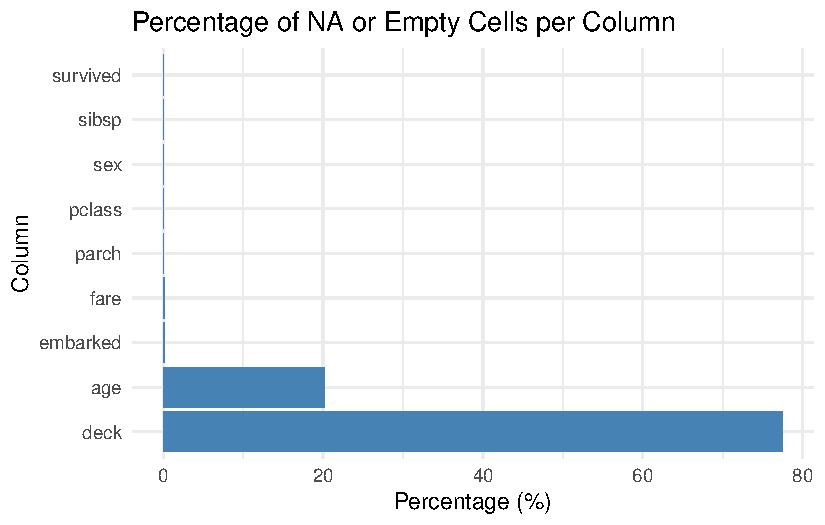
\includegraphics{FinalProject_files/figure-pdf/unnamed-chunk-4-1.pdf}

}

\caption{Percentage of Missing Values}

\end{figure}%

\subsection{Imputing data}\label{imputing-data}

Below we impute Age using the median value in that column.

For deck we use KNN to impute the missing deck values.

After imputing these two columns we can see that the largest amount of
missing data is \textasciitilde0.2\% which is quite small and can be
removed.

\begin{Shaded}
\begin{Highlighting}[]
\CommentTok{\# {-}{-}{-}{-} Age{-}{-}{-}{-}}
\CommentTok{\#Replace NAs in age column with Median value }
\FunctionTok{set.seed}\NormalTok{ (}\DecValTok{1023}\NormalTok{)}
\NormalTok{median\_age }\OtherTok{\textless{}{-}} \FunctionTok{median}\NormalTok{(data.clean}\SpecialCharTok{$}\NormalTok{age, }\AttributeTok{na.rm =} \ConstantTok{TRUE}\NormalTok{)}
\NormalTok{data.clean }\OtherTok{\textless{}{-}}\NormalTok{ data.clean }\SpecialCharTok{\%\textgreater{}\%}
  \FunctionTok{mutate}\NormalTok{(}\AttributeTok{age =} \FunctionTok{ifelse}\NormalTok{(}\FunctionTok{is.na}\NormalTok{(age), median\_age, age))}

\CommentTok{\# {-}{-}{-}{-} deck{-}{-}{-}{-}}
\CommentTok{\# For deck, since its a category, we decided to use KNN  to impute the column:}

\CommentTok{\# Install if not already installed}
\CommentTok{\# install.packages("VIM")}
\FunctionTok{library}\NormalTok{(VIM)}
\end{Highlighting}
\end{Shaded}

\begin{verbatim}
Warning: package 'VIM' was built under R version 4.4.3
\end{verbatim}

\begin{verbatim}
Loading required package: colorspace
\end{verbatim}

\begin{verbatim}
Loading required package: grid
\end{verbatim}

\begin{verbatim}
VIM is ready to use.
\end{verbatim}

\begin{verbatim}
Suggestions and bug-reports can be submitted at: https://github.com/statistikat/VIM/issues
\end{verbatim}

\begin{verbatim}

Attaching package: 'VIM'
\end{verbatim}

\begin{verbatim}
The following object is masked from 'package:datasets':

    sleep
\end{verbatim}

\begin{Shaded}
\begin{Highlighting}[]
\CommentTok{\# Replace "" with NA in the \textquotesingle{}deck\textquotesingle{} column}
\NormalTok{data.clean}\SpecialCharTok{$}\NormalTok{deck[data.clean}\SpecialCharTok{$}\NormalTok{deck }\SpecialCharTok{==} \StringTok{""}\NormalTok{] }\OtherTok{\textless{}{-}} \ConstantTok{NA}

\CommentTok{\# Convert \textquotesingle{}cabin\textquotesingle{} to factor}
\NormalTok{data.clean}\SpecialCharTok{$}\NormalTok{deck }\OtherTok{\textless{}{-}} \FunctionTok{as.factor}\NormalTok{(data.clean}\SpecialCharTok{$}\NormalTok{deck)}

\CommentTok{\# Apply kNN imputation just to Cabin column}
\FunctionTok{set.seed}\NormalTok{ (}\DecValTok{1023}\NormalTok{)}
\NormalTok{data.clean }\OtherTok{\textless{}{-}} \FunctionTok{kNN}\NormalTok{(data.clean, }\AttributeTok{variable =} \StringTok{"deck"}\NormalTok{, }\AttributeTok{k =} \DecValTok{5}\NormalTok{)}

\CommentTok{\# Check that NAs were imputed}
\CommentTok{\# sum(is.na(data.clean$deck))        \# Original}
\CommentTok{\# sum(is.na(data.clean.imputed$deck)) \# After}

\CommentTok{\# Remove indicator col:}
\NormalTok{data.clean}\SpecialCharTok{$}\NormalTok{deck\_imp }\OtherTok{\textless{}{-}} \ConstantTok{NULL}
\end{Highlighting}
\end{Shaded}

\begin{Shaded}
\begin{Highlighting}[]
\DocumentationTok{\#\#\#\#\#\#\#\#\#\#\#\#\#\#\#\#\#\#\#\#\#\#\#\#\#\#\#\#\#\#\#\#\#\#\#\#\#\#\#\#\#\#\#\#\#\#\#\#\#\#\#\#\#\#\#\#\#\#\#\#\#\#\#\#\#\#\#\#\#\#\#\#\#\#\#\#\#\#\#\#}
\CommentTok{\#          Check for Missing values after Imputation                           \#}
\DocumentationTok{\#\#\#\#\#\#\#\#\#\#\#\#\#\#\#\#\#\#\#\#\#\#\#\#\#\#\#\#\#\#\#\#\#\#\#\#\#\#\#\#\#\#\#\#\#\#\#\#\#\#\#\#\#\#\#\#\#\#\#\#\#\#\#\#\#\#\#\#\#\#\#\#\#\#\#\#\#\#\#\#}

\FunctionTok{plot\_missing\_barchart}\NormalTok{(data.clean)}
\end{Highlighting}
\end{Shaded}

\begin{figure}[H]

{\centering 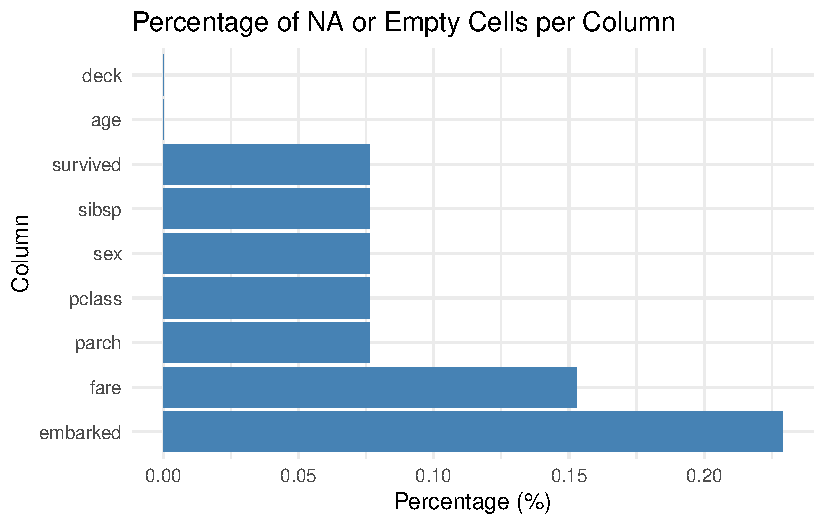
\includegraphics{FinalProject_files/figure-pdf/unnamed-chunk-6-1.pdf}

}

\caption{Percentage of Missing Values after Imputation}

\end{figure}%

\subsection{Dummifying Columns:}\label{dummifying-columns}

We dummify pclass, sex, embarked and deck. We leave sibsp and parch as
continuous variables as we observed that dummifying these columns leads
to smaller significance (See \hyperref[appendix_A]{Appendix A}), whilst
leaving them as continuous maximizes their contributions to the models
explanatory power.

\begin{Shaded}
\begin{Highlighting}[]
\CommentTok{\# Dummifying pclass:}
\NormalTok{data.clean}\SpecialCharTok{$}\NormalTok{pclass\_1 }\OtherTok{=} \FunctionTok{ifelse}\NormalTok{(data.clean}\SpecialCharTok{$}\NormalTok{pclass }\SpecialCharTok{==} \DecValTok{1}\NormalTok{, }\DecValTok{1}\NormalTok{, }\DecValTok{0}\NormalTok{)}
\NormalTok{data.clean}\SpecialCharTok{$}\NormalTok{pclass\_2 }\OtherTok{=} \FunctionTok{ifelse}\NormalTok{(data.clean}\SpecialCharTok{$}\NormalTok{pclass }\SpecialCharTok{==} \DecValTok{2}\NormalTok{, }\DecValTok{1}\NormalTok{, }\DecValTok{0}\NormalTok{)}

\CommentTok{\# Dummifying sex:}
\NormalTok{data.clean}\SpecialCharTok{$}\NormalTok{sex\_M }\OtherTok{=} \FunctionTok{ifelse}\NormalTok{(data.clean}\SpecialCharTok{$}\NormalTok{sex }\SpecialCharTok{==} \StringTok{\textquotesingle{}male\textquotesingle{}}\NormalTok{, }\DecValTok{1}\NormalTok{, }\DecValTok{0}\NormalTok{)}

\CommentTok{\# Dummifying embarked:}
\NormalTok{data.clean}\SpecialCharTok{$}\NormalTok{embarked\_C }\OtherTok{=} \FunctionTok{ifelse}\NormalTok{(data.clean}\SpecialCharTok{$}\NormalTok{embarked }\SpecialCharTok{==} \StringTok{\textquotesingle{}C\textquotesingle{}}\NormalTok{, }\DecValTok{1}\NormalTok{, }\DecValTok{0}\NormalTok{)}
\NormalTok{data.clean}\SpecialCharTok{$}\NormalTok{embarked\_Q }\OtherTok{=} \FunctionTok{ifelse}\NormalTok{(data.clean}\SpecialCharTok{$}\NormalTok{embarked }\SpecialCharTok{==} \StringTok{\textquotesingle{}Q\textquotesingle{}}\NormalTok{, }\DecValTok{1}\NormalTok{, }\DecValTok{0}\NormalTok{)}

\CommentTok{\# Dummifying deck:}
\NormalTok{data.clean}\SpecialCharTok{$}\NormalTok{deck\_A }\OtherTok{=} \FunctionTok{ifelse}\NormalTok{(data.clean}\SpecialCharTok{$}\NormalTok{deck }\SpecialCharTok{==} \StringTok{\textquotesingle{}A\textquotesingle{}}\NormalTok{, }\DecValTok{1}\NormalTok{, }\DecValTok{0}\NormalTok{)}
\NormalTok{data.clean}\SpecialCharTok{$}\NormalTok{deck\_B }\OtherTok{=} \FunctionTok{ifelse}\NormalTok{(data.clean}\SpecialCharTok{$}\NormalTok{deck }\SpecialCharTok{==} \StringTok{\textquotesingle{}B\textquotesingle{}}\NormalTok{, }\DecValTok{1}\NormalTok{, }\DecValTok{0}\NormalTok{)}
\NormalTok{data.clean}\SpecialCharTok{$}\NormalTok{deck\_C }\OtherTok{=} \FunctionTok{ifelse}\NormalTok{(data.clean}\SpecialCharTok{$}\NormalTok{deck }\SpecialCharTok{==} \StringTok{\textquotesingle{}C\textquotesingle{}}\NormalTok{, }\DecValTok{1}\NormalTok{, }\DecValTok{0}\NormalTok{)}
\NormalTok{data.clean}\SpecialCharTok{$}\NormalTok{deck\_D }\OtherTok{=} \FunctionTok{ifelse}\NormalTok{(data.clean}\SpecialCharTok{$}\NormalTok{deck }\SpecialCharTok{==} \StringTok{\textquotesingle{}D\textquotesingle{}}\NormalTok{, }\DecValTok{1}\NormalTok{, }\DecValTok{0}\NormalTok{)}
\NormalTok{data.clean}\SpecialCharTok{$}\NormalTok{deck\_E }\OtherTok{=} \FunctionTok{ifelse}\NormalTok{(data.clean}\SpecialCharTok{$}\NormalTok{deck }\SpecialCharTok{==} \StringTok{\textquotesingle{}E\textquotesingle{}}\NormalTok{, }\DecValTok{1}\NormalTok{, }\DecValTok{0}\NormalTok{)}
\NormalTok{data.clean}\SpecialCharTok{$}\NormalTok{deck\_F }\OtherTok{=} \FunctionTok{ifelse}\NormalTok{(data.clean}\SpecialCharTok{$}\NormalTok{deck }\SpecialCharTok{==} \StringTok{\textquotesingle{}F\textquotesingle{}}\NormalTok{, }\DecValTok{1}\NormalTok{, }\DecValTok{0}\NormalTok{)}
\NormalTok{data.clean}\SpecialCharTok{$}\NormalTok{deck\_G }\OtherTok{=} \FunctionTok{ifelse}\NormalTok{(data.clean}\SpecialCharTok{$}\NormalTok{deck }\SpecialCharTok{==} \StringTok{\textquotesingle{}G\textquotesingle{}}\NormalTok{, }\DecValTok{1}\NormalTok{, }\DecValTok{0}\NormalTok{)}

\CommentTok{\# Removing Dummified cols:}
\NormalTok{data.clean }\OtherTok{=} \FunctionTok{subset}\NormalTok{(data.clean, }\AttributeTok{select  =} \SpecialCharTok{{-}}\FunctionTok{c}\NormalTok{(pclass, sex, embarked,deck))}
\end{Highlighting}
\end{Shaded}

\subsection{Remove NA rows and deck\_G}\label{remove-na-rows-and-deck_g}

Below we remove NA rows, which turned out to be only 2 after proper
cleaning and imputation. We also removed deck\_G as we observed that it
has a large skew in the data distribution with only 13 people allocated
in this deck. It was observed that this variable lead to erroneous
predictions in the model.

\begin{Shaded}
\begin{Highlighting}[]
\CommentTok{\# Plot histogram of the \textquotesingle{}values\textquotesingle{} column}
\FunctionTok{hist}\NormalTok{(data.clean}\SpecialCharTok{$}\NormalTok{deck\_G,}
     \AttributeTok{main =} \StringTok{"Histogram of Values"}\NormalTok{,}
     \AttributeTok{xlab =} \StringTok{"Values"}\NormalTok{,}
     \AttributeTok{col =} \StringTok{"skyblue"}\NormalTok{,}
     \AttributeTok{border =} \StringTok{"white"}\NormalTok{)}
\end{Highlighting}
\end{Shaded}

\begin{figure}[H]

{\centering 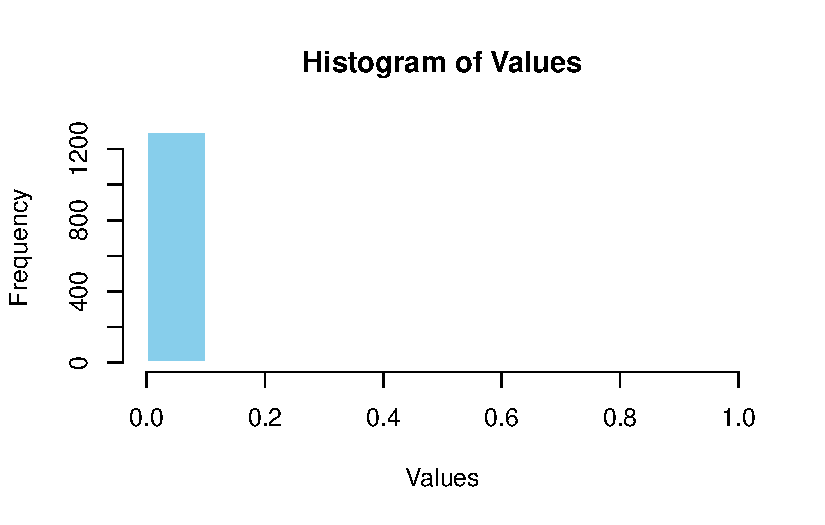
\includegraphics{FinalProject_files/figure-pdf/unnamed-chunk-8-1.pdf}

}

\caption{Histogram of Deck\_G}

\end{figure}%

\begin{Shaded}
\begin{Highlighting}[]
\CommentTok{\# Removing deck\_G col:}
\NormalTok{data.clean }\OtherTok{=} \FunctionTok{subset}\NormalTok{(data.clean, }\AttributeTok{select  =} \SpecialCharTok{{-}}\FunctionTok{c}\NormalTok{(deck\_G))}
\end{Highlighting}
\end{Shaded}

\begin{Shaded}
\begin{Highlighting}[]
\NormalTok{data.clean }\OtherTok{=} \FunctionTok{na.omit}\NormalTok{(data.clean)}
\FunctionTok{cat}\NormalTok{(}\FunctionTok{nrow}\NormalTok{(odata) }\SpecialCharTok{{-}} \FunctionTok{nrow}\NormalTok{(data.clean),}\StringTok{\textquotesingle{}rows were removed from original dataset\textquotesingle{}}\NormalTok{)}
\end{Highlighting}
\end{Shaded}

\begin{verbatim}
2 rows were removed from original dataset
\end{verbatim}

\subsection{Divide into Test / Train}\label{divide-into-test-train}

Finally we divide into 70\% training data and 30\% test data.

\begin{Shaded}
\begin{Highlighting}[]
\FunctionTok{set.seed}\NormalTok{ (}\DecValTok{1023}\NormalTok{)}
\NormalTok{train\_indices }\OtherTok{=} \FunctionTok{sample}\NormalTok{(}\DecValTok{1} \SpecialCharTok{:} \FunctionTok{nrow}\NormalTok{(data.clean), }\AttributeTok{size =} \FloatTok{0.7005}\SpecialCharTok{*}\FunctionTok{nrow}\NormalTok{(data.clean), }\AttributeTok{replace =} \ConstantTok{FALSE}\NormalTok{)}
\NormalTok{train }\OtherTok{=}\NormalTok{ data.clean[train\_indices,]}
\NormalTok{test }\OtherTok{=}\NormalTok{ data.clean[}\SpecialCharTok{{-}}\NormalTok{train\_indices,]}
\FunctionTok{cat}\NormalTok{(}\StringTok{"We are using:"}\NormalTok{, }\FunctionTok{nrow}\NormalTok{(train)}\SpecialCharTok{/}\FunctionTok{nrow}\NormalTok{(data.clean) }\SpecialCharTok{*} \DecValTok{100}\NormalTok{, }\StringTok{\textquotesingle{}\% of the data for training\textquotesingle{}}\NormalTok{)}
\end{Highlighting}
\end{Shaded}

\begin{verbatim}
We are using: 70.03058 % of the data for training
\end{verbatim}

\subsection{EDA}\label{eda}

Using the training data set we use a variety of method to draw some
initial conclusions:

\begin{itemize}
\tightlist
\item
  Histogram: Showing that more people in their late teens up to late
  thirties survived.
\item
  Bar chart showing that more people died than survived
\item
  Bar chart showing that a higher number of people survived when they
  had less siblings on board.
\item
  Correlation matrix shows that sex and Deck\_F are highly negatively
  correlated to survival. There is a soft positive correlation to
  pclass\_1.
\item
  There is a high correlation between pclass\_1 and fare, this justifies
  that one of these predictors can potentially be removed.
\item
  The scatter plots did not give us much more information on the
  relation between the predictors and the dependent variable.
\end{itemize}

\begin{Shaded}
\begin{Highlighting}[]
\CommentTok{\# Histogram showing that more people in their late teens up to late thirties survived.}
\FunctionTok{ggplot}\NormalTok{(train, }\FunctionTok{aes}\NormalTok{(age)) }\SpecialCharTok{+}
  \FunctionTok{geom\_histogram}\NormalTok{(}\AttributeTok{bins=}\DecValTok{30}\NormalTok{)}
\end{Highlighting}
\end{Shaded}

\begin{figure}[H]

{\centering 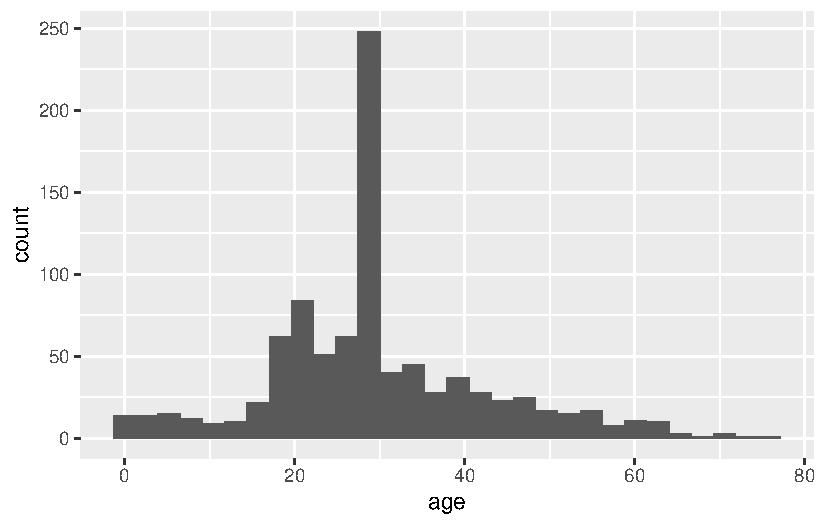
\includegraphics{FinalProject_files/figure-pdf/unnamed-chunk-11-1.pdf}

}

\caption{Histogram of survival vs age}

\end{figure}%

\begin{Shaded}
\begin{Highlighting}[]
\CommentTok{\# Bar chart showing that more people died than survived}
\FunctionTok{ggplot}\NormalTok{(train, }\FunctionTok{aes}\NormalTok{(survived)) }\SpecialCharTok{+}
  \FunctionTok{geom\_bar}\NormalTok{()}
\end{Highlighting}
\end{Shaded}

\begin{figure}[H]

{\centering 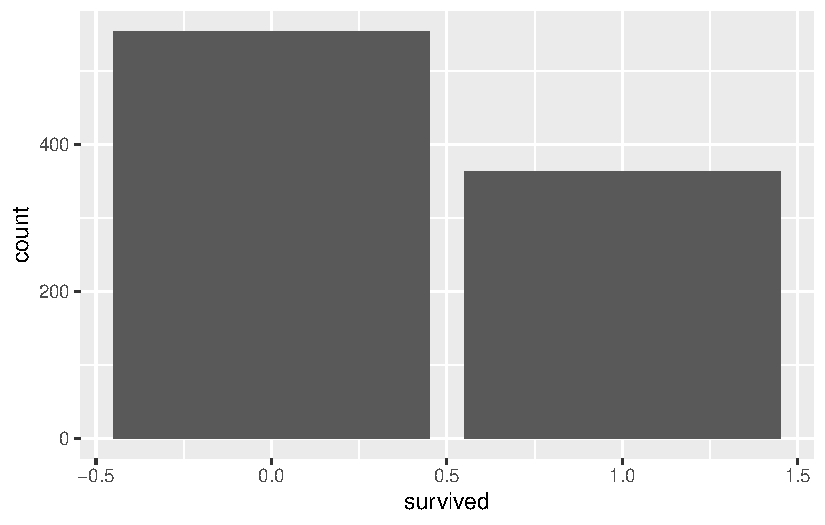
\includegraphics{FinalProject_files/figure-pdf/unnamed-chunk-12-1.pdf}

}

\caption{Barchart of survival}

\end{figure}%

\begin{Shaded}
\begin{Highlighting}[]
\CommentTok{\# Bar chart showing that a higher number of people survived when they had less }
\CommentTok{\# siblings on board.}
\FunctionTok{ggplot}\NormalTok{(train, }\FunctionTok{aes}\NormalTok{(sibsp, survived)) }\SpecialCharTok{+}
  \FunctionTok{geom\_bar}\NormalTok{(}\AttributeTok{stat=}\StringTok{\textquotesingle{}identity\textquotesingle{}}\NormalTok{)}
\end{Highlighting}
\end{Shaded}

\begin{figure}[H]

{\centering 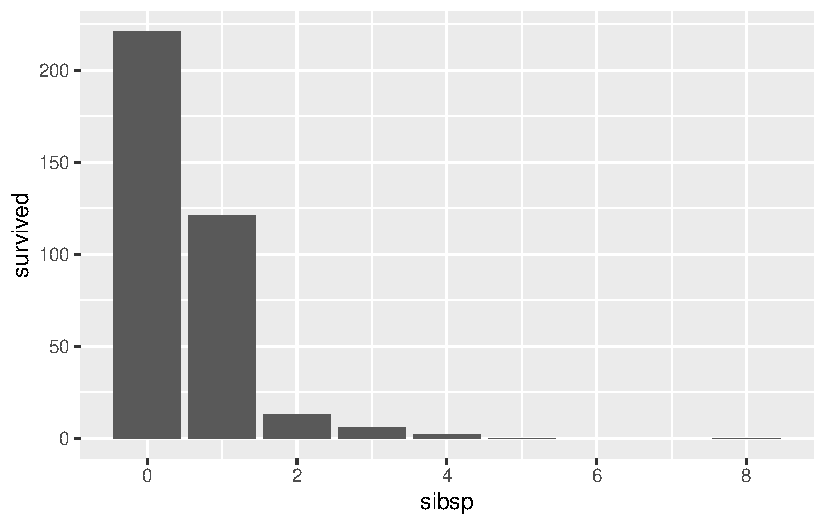
\includegraphics{FinalProject_files/figure-pdf/unnamed-chunk-13-1.pdf}

}

\caption{Barchart of survival vs Num. of siblings}

\end{figure}%

\begin{Shaded}
\begin{Highlighting}[]
\FunctionTok{cor}\NormalTok{(train)}
\end{Highlighting}
\end{Shaded}

\begin{verbatim}
              survived         age       sibsp        parch        fare
survived    1.00000000 -0.04599216 -0.02754365  0.095720424  0.24962042
age        -0.04599216  1.00000000 -0.15495239 -0.122885529  0.16447722
sibsp      -0.02754365 -0.15495239  1.00000000  0.355216328  0.16529618
parch       0.09572042 -0.12288553  0.35521633  1.000000000  0.20987827
fare        0.24962042  0.16447722  0.16529618  0.209878267  1.00000000
pclass_1    0.28432063  0.34847627 -0.02230662 -0.016451014  0.59116304
pclass_2    0.06118909  0.01898825 -0.06908924 -0.017696720 -0.12563735
sex_M      -0.53377358  0.05385130 -0.12706675 -0.243501842 -0.20177640
embarked_C  0.14757622  0.05701305 -0.06121524 -0.001165488  0.27208779
embarked_Q -0.02542950 -0.03373092 -0.06022107 -0.093253422 -0.12699238
deck_A      0.01921839  0.11573201 -0.06315491 -0.054051764  0.06359762
deck_B      0.15658451  0.12638063 -0.01583908  0.076255398  0.45645334
deck_C      0.17861407  0.15235605  0.02822826 -0.049048850  0.30882422
deck_D      0.08437944  0.10150497 -0.02726397 -0.029029703  0.01777467
deck_E      0.33473867  0.11691545 -0.07405912 -0.016332073 -0.01633414
deck_F     -0.47745405 -0.29217392  0.06499841  0.015200439 -0.42777519
              pclass_1    pclass_2       sex_M   embarked_C  embarked_Q
survived    0.28432063  0.06118909 -0.53377358  0.147576220 -0.02542950
age         0.34847627  0.01898825  0.05385130  0.057013047 -0.03373092
sibsp      -0.02230662 -0.06908924 -0.12706675 -0.061215242 -0.06022107
parch      -0.01645101 -0.01769672 -0.24350184 -0.001165488 -0.09325342
fare        0.59116304 -0.12563735 -0.20177640  0.272087792 -0.12699238
pclass_1    1.00000000 -0.30255006 -0.11706927  0.285611052 -0.16373859
pclass_2   -0.30255006  1.00000000 -0.01057862 -0.143425262 -0.14105035
sex_M      -0.11706927 -0.01057862  1.00000000 -0.040151739 -0.09800681
embarked_C  0.28561105 -0.14342526 -0.04015174  1.000000000 -0.16362864
embarked_Q -0.16373859 -0.14105035 -0.09800681 -0.163628636  1.00000000
deck_A      0.28790374 -0.08080438  0.05888172  0.167298858 -0.05745333
deck_B      0.42601897 -0.11327680 -0.09133967  0.182056642 -0.08108169
deck_C      0.48876162 -0.07908768 -0.09801461  0.169699800 -0.08023736
deck_D      0.15200710  0.04093807 -0.03323992  0.248144405 -0.07224766
deck_E      0.05822613 -0.02663532 -0.08900107 -0.078527161 -0.08770239
deck_F     -0.72064119  0.14341225  0.15235799 -0.319688792  0.21273851
                deck_A      deck_B      deck_C      deck_D      deck_E
survived    0.01921839  0.15658451  0.17861407  0.08437944  0.33473867
age         0.11573201  0.12638063  0.15235605  0.10150497  0.11691545
sibsp      -0.06315491 -0.01583908  0.02822826 -0.02726397 -0.07405912
parch      -0.05405176  0.07625540 -0.04904885 -0.02902970 -0.01633207
fare        0.06359762  0.45645334  0.30882422  0.01777467 -0.01633414
pclass_1    0.28790374  0.42601897  0.48876162  0.15200710  0.05822613
pclass_2   -0.08080438 -0.11327680 -0.07908768  0.04093807 -0.02663532
sex_M       0.05888172 -0.09133967 -0.09801461 -0.03323992 -0.08900107
embarked_C  0.16729886  0.18205664  0.16969980  0.24814440 -0.07852716
embarked_Q -0.05745333 -0.08108169 -0.08023736 -0.07224766 -0.08770239
deck_A      1.00000000 -0.04614047 -0.06005247 -0.04955727 -0.06365303
deck_B     -0.04614047  1.00000000 -0.08474977 -0.06993828 -0.08983109
deck_C     -0.06005247 -0.08474977  1.00000000 -0.09102568 -0.11691645
deck_D     -0.04955727 -0.06993828 -0.09102568  1.00000000 -0.09648328
deck_E     -0.06365303 -0.08983109 -0.11691645 -0.09648328  1.00000000
deck_F     -0.22835159 -0.32226388 -0.41943104 -0.34612824 -0.44457878
                deck_F
survived   -0.47745405
age        -0.29217392
sibsp       0.06499841
parch       0.01520044
fare       -0.42777519
pclass_1   -0.72064119
pclass_2    0.14341225
sex_M       0.15235799
embarked_C -0.31968879
embarked_Q  0.21273851
deck_A     -0.22835159
deck_B     -0.32226388
deck_C     -0.41943104
deck_D     -0.34612824
deck_E     -0.44457878
deck_F      1.00000000
\end{verbatim}

\begin{Shaded}
\begin{Highlighting}[]
\FunctionTok{pairs}\NormalTok{(train[}\FunctionTok{c}\NormalTok{(}\DecValTok{1}\SpecialCharTok{:}\DecValTok{4}\NormalTok{,}\DecValTok{7}\NormalTok{,}\DecValTok{13}\NormalTok{)])}
\end{Highlighting}
\end{Shaded}

\begin{figure}[H]

{\centering 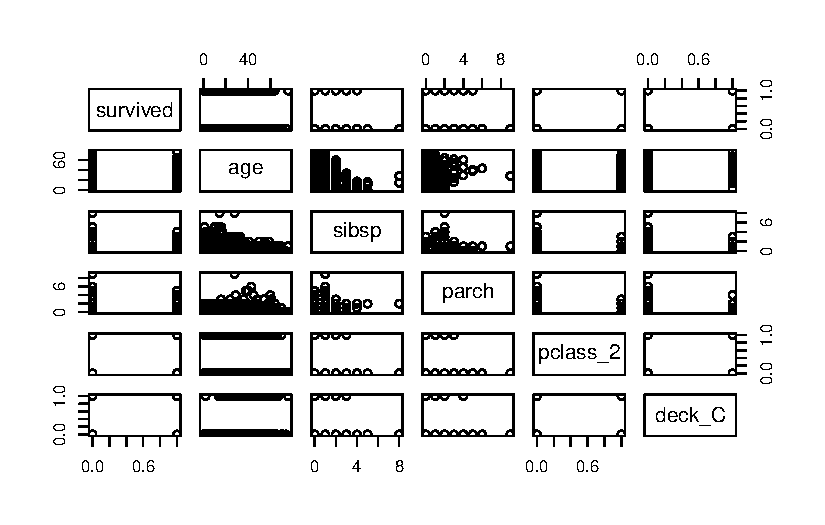
\includegraphics{FinalProject_files/figure-pdf/unnamed-chunk-14-1.pdf}

}

\caption{Scatter plots of all variables in train data}

\end{figure}%

\begin{Shaded}
\begin{Highlighting}[]
\CommentTok{\# Since this data is mainly categorical, the scatterplot and correlation matrix are not very useful.}
\end{Highlighting}
\end{Shaded}

(Statology, 2025) is used to develop the correlation values between our
categorical columns. This describes the use of pysch and rcompanion.

\begin{Shaded}
\begin{Highlighting}[]
\CommentTok{\#install.packages("psych")}
\FunctionTok{library}\NormalTok{(psych) }\CommentTok{\# [@statology2025] to understand how this works}
\end{Highlighting}
\end{Shaded}

\begin{verbatim}
Warning: package 'psych' was built under R version 4.4.3
\end{verbatim}

\begin{verbatim}

Attaching package: 'psych'
\end{verbatim}

\begin{verbatim}
The following objects are masked from 'package:ggplot2':

    %+%, alpha
\end{verbatim}

\begin{Shaded}
\begin{Highlighting}[]
\FunctionTok{tetrachoric}\NormalTok{(train[, }\FunctionTok{c}\NormalTok{(}\StringTok{"survived"}\NormalTok{, }\StringTok{"sex\_M"}\NormalTok{)])}
\end{Highlighting}
\end{Shaded}

\begin{verbatim}
Call: tetrachoric(x = train[, c("survived", "sex_M")])
tetrachoric correlation 
         srvvd sex_M
survived  1.00      
sex_M    -0.75  1.00

 with tau of 
survived    sex_M 
    0.26    -0.35 
\end{verbatim}

\begin{Shaded}
\begin{Highlighting}[]
\FunctionTok{tetrachoric}\NormalTok{(train[, }\FunctionTok{c}\NormalTok{(}\StringTok{"survived"}\NormalTok{, }\StringTok{"pclass\_1"}\NormalTok{)])}
\end{Highlighting}
\end{Shaded}

\begin{verbatim}
Call: tetrachoric(x = train[, c("survived", "pclass_1")])
tetrachoric correlation 
         srvvd pcl_1
survived 1.00       
pclass_1 0.46  1.00 

 with tau of 
survived pclass_1 
    0.26     0.69 
\end{verbatim}

\begin{Shaded}
\begin{Highlighting}[]
\FunctionTok{tetrachoric}\NormalTok{(train[, }\FunctionTok{c}\NormalTok{(}\StringTok{"survived"}\NormalTok{, }\StringTok{"pclass\_2"}\NormalTok{)])}
\end{Highlighting}
\end{Shaded}

\begin{verbatim}
Call: tetrachoric(x = train[, c("survived", "pclass_2")])
tetrachoric correlation 
         srvvd pcl_2
survived 1.00       
pclass_2 0.11  1.00 

 with tau of 
survived pclass_2 
    0.26     0.77 
\end{verbatim}

\begin{Shaded}
\begin{Highlighting}[]
\CommentTok{\#install.packages("rcompanion")}
\FunctionTok{library}\NormalTok{(rcompanion) }\CommentTok{\# Reference 4 to understand how this works.}
\end{Highlighting}
\end{Shaded}

\begin{verbatim}
Warning: package 'rcompanion' was built under R version 4.4.3
\end{verbatim}

\begin{verbatim}

Attaching package: 'rcompanion'
\end{verbatim}

\begin{verbatim}
The following object is masked from 'package:psych':

    phi
\end{verbatim}

\begin{Shaded}
\begin{Highlighting}[]
\FunctionTok{cramerV}\NormalTok{(train}\SpecialCharTok{$}\NormalTok{survived, train}\SpecialCharTok{$}\NormalTok{sex)}
\end{Highlighting}
\end{Shaded}

\begin{verbatim}
Cramer V 
  0.5338 
\end{verbatim}

\begin{Shaded}
\begin{Highlighting}[]
\FunctionTok{library}\NormalTok{(corrplot)}
\end{Highlighting}
\end{Shaded}

\begin{verbatim}
corrplot 0.95 loaded
\end{verbatim}

\begin{Shaded}
\begin{Highlighting}[]
\NormalTok{cor\_matrix }\OtherTok{\textless{}{-}} \FunctionTok{cor}\NormalTok{(train)}\CommentTok{\#[,1]}
\FunctionTok{corrplot}\NormalTok{(cor\_matrix, }\AttributeTok{method =} \StringTok{"circle"}\NormalTok{)}
\end{Highlighting}
\end{Shaded}

\begin{figure}[H]

{\centering 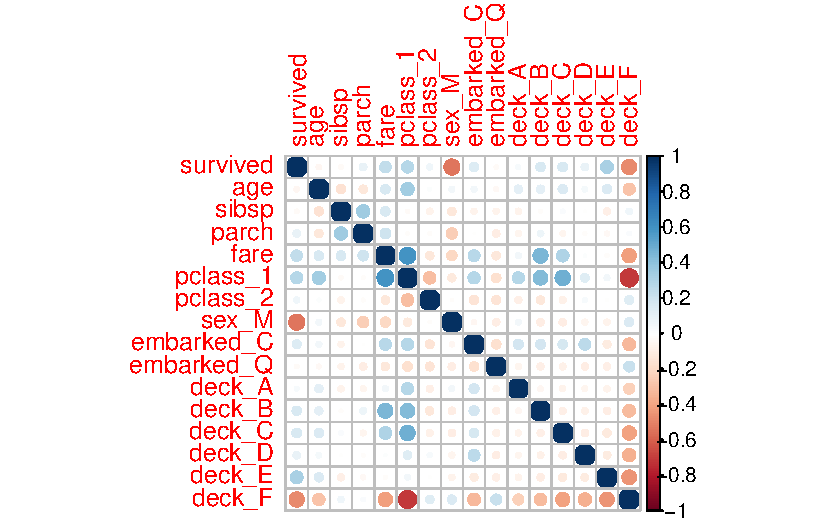
\includegraphics{FinalProject_files/figure-pdf/unnamed-chunk-16-1.pdf}

}

\caption{Correlation Matrix}

\end{figure}%

\section{Model Development Process}\label{model-development-process}

The data was properly cleaned and divided into train/test in the prior
section.

Here we train a binary model. The Q-Q plot shows that the residuals are
indeed normally distributed so a transformation is potentially not
necessary.

The statistical comparison between test and train data shows that the
model is very stable with an accuracy of \textasciitilde84\% for both.

We also analyzed the VIF and we see that there is high degree of
correlation between the decks, this provides justification to remove
some of the decks as predictors.

\begin{Shaded}
\begin{Highlighting}[]
\FunctionTok{library}\NormalTok{(car)}
\end{Highlighting}
\end{Shaded}

\begin{verbatim}
Warning: package 'car' was built under R version 4.4.3
\end{verbatim}

\begin{verbatim}
Loading required package: carData
\end{verbatim}

\begin{verbatim}
Warning: package 'carData' was built under R version 4.4.3
\end{verbatim}

\begin{verbatim}

Attaching package: 'car'
\end{verbatim}

\begin{verbatim}
The following object is masked from 'package:psych':

    logit
\end{verbatim}

\begin{verbatim}
The following object is masked from 'package:dplyr':

    recode
\end{verbatim}

\begin{verbatim}
The following object is masked from 'package:purrr':

    some
\end{verbatim}

\begin{Shaded}
\begin{Highlighting}[]
\CommentTok{\# Log model on train data:}
\FunctionTok{set.seed}\NormalTok{ (}\DecValTok{1023}\NormalTok{)}
\NormalTok{lmod }\OtherTok{\textless{}{-}} \FunctionTok{glm}\NormalTok{(survived }\SpecialCharTok{\textasciitilde{}}\NormalTok{ ., }\AttributeTok{family =}\NormalTok{ binomial, }\AttributeTok{data =}\NormalTok{ train)}
\CommentTok{\# summary(lmod)}
\FunctionTok{vif}\NormalTok{(lmod)}
\end{Highlighting}
\end{Shaded}

\begin{verbatim}
       age      sibsp      parch       fare   pclass_1   pclass_2      sex_M 
  1.487819   1.241500   1.283338   1.720620   4.661296   1.574259   1.619104 
embarked_C embarked_Q     deck_A     deck_B     deck_C     deck_D     deck_E 
  1.433942   1.368562   5.122014   6.161202   9.446197   7.824253   7.280808 
    deck_F 
 18.174852 
\end{verbatim}

\begin{Shaded}
\begin{Highlighting}[]
\NormalTok{y\_hat\_log\_train }\OtherTok{\textless{}{-}} \FunctionTok{predict}\NormalTok{(lmod, }\AttributeTok{data =}\NormalTok{ train, }\AttributeTok{type=}\StringTok{"response"}\NormalTok{)}
\NormalTok{predictions\_log\_train }\OtherTok{\textless{}{-}} \FunctionTok{ifelse}\NormalTok{(y\_hat\_log\_train }\SpecialCharTok{\textgreater{}} \FloatTok{0.5}\NormalTok{, }\DecValTok{1}\NormalTok{, }\DecValTok{0}\NormalTok{)}

\NormalTok{y\_hat\_log\_test}\OtherTok{\textless{}{-}}\FunctionTok{predict}\NormalTok{(lmod, }\AttributeTok{newdata =}\NormalTok{ test, }\AttributeTok{type=}\StringTok{"response"}\NormalTok{)}
\NormalTok{predictions\_log\_test }\OtherTok{\textless{}{-}} \FunctionTok{ifelse}\NormalTok{(y\_hat\_log\_test }\SpecialCharTok{\textgreater{}} \FloatTok{0.5}\NormalTok{, }\DecValTok{1}\NormalTok{, }\DecValTok{0}\NormalTok{)}

\NormalTok{confusion\_matrix\_log\_train }\OtherTok{\textless{}{-}} \FunctionTok{confusionMatrix}\NormalTok{(}\FunctionTok{as.factor}\NormalTok{(predictions\_log\_train), }\FunctionTok{as.factor}\NormalTok{(train}\SpecialCharTok{$}\NormalTok{survived),}\AttributeTok{mode=}\StringTok{"prec\_recall"}\NormalTok{, }\AttributeTok{positive =} \StringTok{"1"}\NormalTok{)}
\NormalTok{base.model.accuracy }\OtherTok{=}\NormalTok{ confusion\_matrix\_log\_train}\SpecialCharTok{$}\NormalTok{overall[}\StringTok{\textquotesingle{}Accuracy\textquotesingle{}}\NormalTok{]}
\NormalTok{base.model.f1 }\OtherTok{=}\NormalTok{ confusion\_matrix\_log\_train}\SpecialCharTok{$}\NormalTok{byClass[}\StringTok{\textquotesingle{}F1\textquotesingle{}}\NormalTok{]}
\NormalTok{base.model.train.summary }\OtherTok{=} \FunctionTok{data.frame}\NormalTok{(}
  \AttributeTok{Accuracy =}\NormalTok{ base.model.accuracy,}
  \AttributeTok{F1 =}\NormalTok{ base.model.f1}
\NormalTok{)}
\FunctionTok{row.names}\NormalTok{(base.model.train.summary) }\OtherTok{\textless{}{-}} \StringTok{\textquotesingle{}base.model.train\textquotesingle{}}  



\NormalTok{confusion\_matrix\_log\_test }\OtherTok{\textless{}{-}} \FunctionTok{confusionMatrix}\NormalTok{(}\FunctionTok{as.factor}\NormalTok{(predictions\_log\_test), }\FunctionTok{as.factor}\NormalTok{(test}\SpecialCharTok{$}\NormalTok{survived),}\AttributeTok{mode=}\StringTok{"prec\_recall"}\NormalTok{, }\AttributeTok{positive =} \StringTok{"1"}\NormalTok{)}
\NormalTok{base.model.accuracy }\OtherTok{=}\NormalTok{ confusion\_matrix\_log\_test}\SpecialCharTok{$}\NormalTok{overall[}\StringTok{\textquotesingle{}Accuracy\textquotesingle{}}\NormalTok{]}
\NormalTok{base.model.f1 }\OtherTok{=}\NormalTok{ confusion\_matrix\_log\_test}\SpecialCharTok{$}\NormalTok{byClass[}\StringTok{\textquotesingle{}F1\textquotesingle{}}\NormalTok{]}
\NormalTok{base.model.test.summary }\OtherTok{=} \FunctionTok{data.frame}\NormalTok{(}
  \AttributeTok{Accuracy =}\NormalTok{ base.model.accuracy,}
  \AttributeTok{F1 =}\NormalTok{ base.model.f1}
\NormalTok{)}
\FunctionTok{row.names}\NormalTok{(base.model.test.summary) }\OtherTok{\textless{}{-}} \StringTok{\textquotesingle{}base.model.test\textquotesingle{}}
\end{Highlighting}
\end{Shaded}

\begin{Shaded}
\begin{Highlighting}[]
\FunctionTok{data.frame}\NormalTok{(}\FunctionTok{rbind}\NormalTok{(base.model.train.summary, base.model.test.summary))}
\end{Highlighting}
\end{Shaded}

\begin{longtable}[]{@{}lrr@{}}
\caption{Summary Stats. of base log. model}\tabularnewline
\toprule\noalign{}
& Accuracy & F1 \\
\midrule\noalign{}
\endfirsthead
\toprule\noalign{}
& Accuracy & F1 \\
\midrule\noalign{}
\endhead
\bottomrule\noalign{}
\endlastfoot
base.model.train & 0.8504367 & 0.8115543 \\
base.model.test & 0.8392857 & 0.7758007 \\
\end{longtable}

\begin{Shaded}
\begin{Highlighting}[]
\FunctionTok{summary}\NormalTok{(lmod)}
\end{Highlighting}
\end{Shaded}

\begin{verbatim}

Call:
glm(formula = survived ~ ., family = binomial, data = train)

Coefficients:
              Estimate Std. Error z value Pr(>|z|)    
(Intercept)  5.386e+00  8.913e-01   6.042 1.52e-09 ***
age         -5.396e-02  9.051e-03  -5.962 2.49e-09 ***
sibsp       -2.538e-01  1.205e-01  -2.106  0.03520 *  
parch        1.371e-02  1.185e-01   0.116  0.90790    
fare        -6.976e-05  2.289e-03  -0.030  0.97568    
pclass_1     7.953e-01  4.670e-01   1.703  0.08856 .  
pclass_2     1.829e+00  3.011e-01   6.073 1.25e-09 ***
sex_M       -3.274e+00  2.566e-01 -12.756  < 2e-16 ***
embarked_C   8.299e-01  2.877e-01   2.884  0.00393 ** 
embarked_Q   7.944e-01  3.602e-01   2.205  0.02744 *  
deck_A      -2.166e+00  1.011e+00  -2.143  0.03212 *  
deck_B      -1.510e+00  1.006e+00  -1.501  0.13338    
deck_C      -1.646e+00  9.553e-01  -1.723  0.08484 .  
deck_D      -2.616e+00  9.310e-01  -2.810  0.00495 ** 
deck_E       4.274e-01  8.975e-01   0.476  0.63393    
deck_F      -4.342e+00  8.572e-01  -5.065 4.08e-07 ***
---
Signif. codes:  0 '***' 0.001 '**' 0.01 '*' 0.05 '.' 0.1 ' ' 1

(Dispersion parameter for binomial family taken to be 1)

    Null deviance: 1230.15  on 915  degrees of freedom
Residual deviance:  634.78  on 900  degrees of freedom
AIC: 666.78

Number of Fisher Scoring iterations: 6
\end{verbatim}

\begin{Shaded}
\begin{Highlighting}[]
\FunctionTok{par}\NormalTok{(}\AttributeTok{mfrow=}\FunctionTok{c}\NormalTok{(}\DecValTok{2}\NormalTok{,}\DecValTok{2}\NormalTok{))}
\FunctionTok{plot}\NormalTok{(lmod)}
\end{Highlighting}
\end{Shaded}

\begin{figure}[H]

{\centering 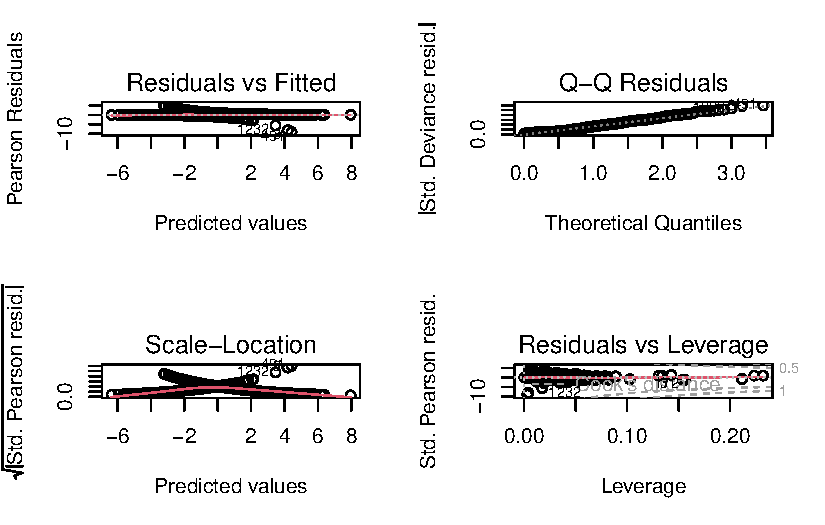
\includegraphics{FinalProject_files/figure-pdf/unnamed-chunk-21-1.pdf}

}

\caption{4x4 standard plots for log. model}

\end{figure}%

\begin{Shaded}
\begin{Highlighting}[]
\CommentTok{\# Plots show that a linear model is not appropriate for this data.}
\end{Highlighting}
\end{Shaded}

\section{Model Performance Testing}\label{model-performance-testing}

We compare four different models:

1) Base log. model (lmod)

2) Model with insig. pred. removed (filtered.model)

3) Stepwise model (step.model)

4) Model with high vif pred. removed (vif.model)

When comparing the accuracy and F1 score on all models the filtered
model was the highest performer and we decided to use that as the
champion model until now. We suspect that multicollinearity among the
decks has an impact on the model performance which is why removing these
collinear predictors and filtering for insignificant variables improved
the model slightly against the based model (+0.3\%).

\begin{Shaded}
\begin{Highlighting}[]
\DocumentationTok{\#\#\#\#\#\#\#\#\#\#\#\#\#\#\#\#\#\#\#\#\#\#\#\#\#\#\#\#\#\#\#\#\#\#\#\#\#\#\#\#\#\#\#\#\#\#\#\#\#\#\#\#\#\#\#\#\#\#\#\#\#\#\#\#\#\#\#\#\#\#\#\#\#\#\#\#\#\#\#\#}
\CommentTok{\#              Function to remove Insig. Predictors one by one                 \# }
\DocumentationTok{\#\#\#\#\#\#\#\#\#\#\#\#\#\#\#\#\#\#\#\#\#\#\#\#\#\#\#\#\#\#\#\#\#\#\#\#\#\#\#\#\#\#\#\#\#\#\#\#\#\#\#\#\#\#\#\#\#\#\#\#\#\#\#\#\#\#\#\#\#\#\#\#\#\#\#\#\#\#\#\#}

\NormalTok{backward\_eliminate }\OtherTok{=} \ControlFlowTok{function}\NormalTok{(model, }\AttributeTok{alpha =} \FloatTok{0.05}\NormalTok{) \{}
  \ControlFlowTok{repeat}\NormalTok{ \{}
\NormalTok{    d1 }\OtherTok{=} \FunctionTok{drop1}\NormalTok{(model, }\AttributeTok{test =} \StringTok{"F"}\NormalTok{)}
    
    \CommentTok{\# Get p{-}values excluding intercept row}
\NormalTok{    pvals }\OtherTok{=}\NormalTok{ d1}\SpecialCharTok{$}\StringTok{\textasciigrave{}}\AttributeTok{Pr(\textgreater{}F)}\StringTok{\textasciigrave{}}\NormalTok{[}\SpecialCharTok{{-}}\DecValTok{1}\NormalTok{]}
    
    \CommentTok{\# Stop if all predictors are significant or only intercept left}
    \ControlFlowTok{if}\NormalTok{( }\FunctionTok{all}\NormalTok{(}\FunctionTok{is.na}\NormalTok{(pvals)) }\SpecialCharTok{||} \FunctionTok{max}\NormalTok{(pvals, }\AttributeTok{na.rm =} \ConstantTok{TRUE}\NormalTok{) }\SpecialCharTok{\textless{}=}\NormalTok{ alpha )\{}
      \FunctionTok{print}\NormalTok{(}\StringTok{"all variable are signifcant"}\NormalTok{)}
      \ControlFlowTok{break}
\NormalTok{    \} }
    
    \CommentTok{\# Remove the term with max p{-}value}
\NormalTok{    term\_to\_remove }\OtherTok{=} \FunctionTok{rownames}\NormalTok{(d1)[}\SpecialCharTok{{-}}\DecValTok{1}\NormalTok{][}\FunctionTok{which.max}\NormalTok{(pvals)]}
    \FunctionTok{cat}\NormalTok{(}\StringTok{"Removing:"}\NormalTok{, term\_to\_remove, }\StringTok{"with p{-}value"}\NormalTok{, }\FunctionTok{max}\NormalTok{(pvals, }\AttributeTok{na.rm =} \ConstantTok{TRUE}\NormalTok{), }\StringTok{"}\SpecialCharTok{\textbackslash{}n}\StringTok{"}\NormalTok{)}
\NormalTok{    model }\OtherTok{=} \FunctionTok{update}\NormalTok{(model, }\FunctionTok{paste}\NormalTok{(}\StringTok{". \textasciitilde{} . {-}"}\NormalTok{, term\_to\_remove))}
\NormalTok{  \}}
  \FunctionTok{return}\NormalTok{(model)}
\NormalTok{\}}
\end{Highlighting}
\end{Shaded}

\begin{Shaded}
\begin{Highlighting}[]
\DocumentationTok{\#\#\#\#\#\#\#\#\#\#\#\#\#\#\#\#\#\#\#\#\#\#\#\#\#\#\#\#\#\#\#\#\#\#\#\#\#\#\#\#\#\#\#\#\#\#\#\#\#\#\#\#\#\#\#\#\#\#\#\#\#\#\#\#\#\#\#\#\#\#\#\#\#\#\#\#\#\#\#\#}
\CommentTok{\#                     Function to remove Cooks Outliers                        \# }
\DocumentationTok{\#\#\#\#\#\#\#\#\#\#\#\#\#\#\#\#\#\#\#\#\#\#\#\#\#\#\#\#\#\#\#\#\#\#\#\#\#\#\#\#\#\#\#\#\#\#\#\#\#\#\#\#\#\#\#\#\#\#\#\#\#\#\#\#\#\#\#\#\#\#\#\#\#\#\#\#\#\#\#\#                        }
\CommentTok{\# model\_formula: A formula object, e.g. PSA.level \textasciitilde{} .}
\CommentTok{\# data: A data frame containing the variables in the model.}
\CommentTok{\# threshold: A numeric value indicating the Cook\textquotesingle{}s D threshold (default 0.5).}
\CommentTok{\# print: If TRUE (default) will print the rows beign removed.}
\CommentTok{\# returns: A list with the final model and the filtered dataset.}
\CommentTok{\# }
\CommentTok{\# Example usage:}
\CommentTok{\# result = remove\_cooks\_outliers(PSA.level \textasciitilde{} ., mydata)}
\CommentTok{\# summary(result$model)}
\CommentTok{\# str(result$filtered\_data)}
\NormalTok{remove\_cooks\_outliers }\OtherTok{=} \ControlFlowTok{function}\NormalTok{(model\_formula, data, }\AttributeTok{threshold =} \FloatTok{0.5}\NormalTok{, }
                                 \AttributeTok{print =} \ConstantTok{TRUE}\NormalTok{) }
\NormalTok{  \{}
  
\NormalTok{  all\_high\_cd\_rows }\OtherTok{=} \FunctionTok{data.frame}\NormalTok{()  }\CommentTok{\# to store all removed rows}

  \ControlFlowTok{repeat}\NormalTok{ \{}
\NormalTok{    model }\OtherTok{=} \FunctionTok{glm}\NormalTok{(model\_formula, }\AttributeTok{family =}\NormalTok{ binomial, }\AttributeTok{data =}\NormalTok{ data) }
\NormalTok{    cooksD }\OtherTok{=} \FunctionTok{cooks.distance}\NormalTok{(model)}
\NormalTok{    high\_cd\_indices }\OtherTok{=} \FunctionTok{which}\NormalTok{(cooksD }\SpecialCharTok{\textgreater{}}\NormalTok{ threshold)}
    
    \ControlFlowTok{if}\NormalTok{ (}\FunctionTok{length}\NormalTok{(high\_cd\_indices) }\SpecialCharTok{==} \DecValTok{0}\NormalTok{) \{ }\CommentTok{\# If there are no more outliers}
      \ControlFlowTok{break}
\NormalTok{    \}}
    
    \ControlFlowTok{if}\NormalTok{ (print }\SpecialCharTok{==} \ConstantTok{TRUE}\NormalTok{)\{}
      \FunctionTok{cat}\NormalTok{(}\StringTok{"Removing rows with Cook\textquotesingle{}s D \textgreater{}"}\NormalTok{, threshold, }\StringTok{":}\SpecialCharTok{\textbackslash{}n}\StringTok{"}\NormalTok{, high\_cd\_indices, }\StringTok{"}\SpecialCharTok{\textbackslash{}n}\StringTok{"}\NormalTok{)}
\NormalTok{    \}}
    \CommentTok{\# Save these outliers before removing them}
\NormalTok{    high\_cd\_rows }\OtherTok{=}\NormalTok{ data[high\_cd\_indices, ]}
\NormalTok{    all\_high\_cd\_rows }\OtherTok{=} \FunctionTok{rbind}\NormalTok{(all\_high\_cd\_rows, high\_cd\_rows)}
    
    \CommentTok{\# Update data by removing high CD rows for next iteration.}
\NormalTok{    data }\OtherTok{=}\NormalTok{ data[}\SpecialCharTok{{-}}\NormalTok{high\_cd\_indices, ]}
\NormalTok{  \}}
  
\NormalTok{  final\_model }\OtherTok{=} \FunctionTok{glm}\NormalTok{(model\_formula, }\AttributeTok{family =}\NormalTok{ binomial, }\AttributeTok{data =}\NormalTok{ data)}
  \FunctionTok{return}\NormalTok{(}\FunctionTok{list}\NormalTok{(}\AttributeTok{model =}\NormalTok{ final\_model, }\AttributeTok{filtered\_data =}\NormalTok{ data, }\AttributeTok{high\_cd\_data =}\NormalTok{ all\_high\_cd\_rows))}
\NormalTok{\}}
\end{Highlighting}
\end{Shaded}

\begin{Shaded}
\begin{Highlighting}[]
\DocumentationTok{\#\#\#\#\#\#\#\#\#\#\#\#\#\#\#\#\#\#\#\#\#\#\#\#\#\#\#\#\#\#\#\#\#\#\#\#\#\#\#\#\#\#\#\#\#\#\#\#\#\#\#\#\#\#\#\#\#\#\#\#\#\#\#\#\#\#\#\#\#\#\#\#\#\#\#\#\#\#\#\#}
\CommentTok{\#                    Model with insig. variables removed                      \# }
\DocumentationTok{\#\#\#\#\#\#\#\#\#\#\#\#\#\#\#\#\#\#\#\#\#\#\#\#\#\#\#\#\#\#\#\#\#\#\#\#\#\#\#\#\#\#\#\#\#\#\#\#\#\#\#\#\#\#\#\#\#\#\#\#\#\#\#\#\#\#\#\#\#\#\#\#\#\#\#\#\#\#\#\#}
\NormalTok{binary.model.filtered }\OtherTok{=} \FunctionTok{backward\_eliminate}\NormalTok{(lmod)}
\end{Highlighting}
\end{Shaded}

\begin{verbatim}
Warning in drop1.glm(model, test = "F"): F test assumes 'quasibinomial' family
\end{verbatim}

\begin{verbatim}
Removing: fare with p-value 0.9710719 
\end{verbatim}

\begin{verbatim}
Warning in drop1.glm(model, test = "F"): F test assumes 'quasibinomial' family
\end{verbatim}

\begin{verbatim}
Removing: parch with p-value 0.894389 
\end{verbatim}

\begin{verbatim}
Warning in drop1.glm(model, test = "F"): F test assumes 'quasibinomial' family
\end{verbatim}

\begin{verbatim}
Removing: deck_E with p-value 0.5871368 
\end{verbatim}

\begin{verbatim}
Warning in drop1.glm(model, test = "F"): F test assumes 'quasibinomial' family
\end{verbatim}

\begin{verbatim}
[1] "all variable are signifcant"
\end{verbatim}

\begin{Shaded}
\begin{Highlighting}[]
\DocumentationTok{\#\#\#\#\#\#\#\#\#\#\#\#\#\#\#\#\#\#\#\#\#\#\#\#\#\#\#\#\#\#\#\#\#\#\#\#\#\#\#\#\#\#\#\#\#\#\#\#\#\#\#\#\#\#\#\#\#\#\#\#\#\#\#\#\#\#\#\#\#\#\#\#\#\#\#\#\#\#\#\#}
\CommentTok{\#                step wise model with insig. variables removed                 \# }
\DocumentationTok{\#\#\#\#\#\#\#\#\#\#\#\#\#\#\#\#\#\#\#\#\#\#\#\#\#\#\#\#\#\#\#\#\#\#\#\#\#\#\#\#\#\#\#\#\#\#\#\#\#\#\#\#\#\#\#\#\#\#\#\#\#\#\#\#\#\#\#\#\#\#\#\#\#\#\#\#\#\#\#\#}
\FunctionTok{library}\NormalTok{(olsrr)}
\end{Highlighting}
\end{Shaded}

\begin{verbatim}
Warning: package 'olsrr' was built under R version 4.4.3
\end{verbatim}

\begin{verbatim}

Attaching package: 'olsrr'
\end{verbatim}

\begin{verbatim}
The following object is masked from 'package:MASS':

    cement
\end{verbatim}

\begin{verbatim}
The following object is masked from 'package:datasets':

    rivers
\end{verbatim}

\begin{Shaded}
\begin{Highlighting}[]
\FunctionTok{ols\_step\_both\_p}\NormalTok{(lmod,}\AttributeTok{p\_enter=}\FloatTok{0.1}\NormalTok{,}\AttributeTok{p\_remove=}\FloatTok{0.05}\NormalTok{,}\AttributeTok{details=}\ConstantTok{FALSE}\NormalTok{)}
\end{Highlighting}
\end{Shaded}

\begin{verbatim}

                                    Stepwise Summary                                    
--------------------------------------------------------------------------------------
Step    Variable            AIC         SBC            SBIC           R2       Adj. R2 
--------------------------------------------------------------------------------------
 0      Base Model        1293.366    1303.006     -28281799.310    0.00000    0.00000 
 1      sex_M (+)          988.183    1002.643     -55309468.385    0.28491    0.28413 
 2      deck_F (+)         757.110     776.390     -92005909.772    0.44556    0.44435 
 3      age (+)            723.096     747.196     -99521155.302    0.46694    0.46518 
 4      pclass_2 (+)       697.456     726.376    -105700242.392    0.48278    0.48051 
 5      deck_E (+)         674.236     707.976    -111671761.113    0.49683    0.49406 
 6      sibsp (+)          668.302     706.862    -113609066.331    0.50117    0.49788 
 7      deck_D (+)         664.319     707.699    -115088607.776    0.50442    0.50059 
 8      embarked_Q (+)     663.468     711.668    -115792422.465    0.50596    0.50160 
 9      embarked_Q (-)     664.319     707.699    -115088607.776    0.50442    0.50059 
--------------------------------------------------------------------------------------

Final Model Output 
------------------

                         Model Summary                          
---------------------------------------------------------------
R                       0.710       RMSE                 0.344 
R-Squared               0.504       MSE                  0.119 
Adj. R-Squared          0.501       Coef. Var           87.272 
Pred R-Squared          0.495       AIC                664.319 
MAE                     0.262       SBC                707.699 
---------------------------------------------------------------
 RMSE: Root Mean Square Error 
 MSE: Mean Square Error 
 MAE: Mean Absolute Error 
 AIC: Akaike Information Criteria 
 SBC: Schwarz Bayesian Criteria 

                                ANOVA                                 
---------------------------------------------------------------------
               Sum of                                                
              Squares         DF    Mean Square       F         Sig. 
---------------------------------------------------------------------
Regression    110.541          7         15.792    132.026    0.0000 
Residual      108.606        908          0.120                      
Total         219.147        915                                     
---------------------------------------------------------------------

                                   Parameter Estimates                                    
-----------------------------------------------------------------------------------------
      model      Beta    Std. Error    Std. Beta       t        Sig      lower     upper 
-----------------------------------------------------------------------------------------
(Intercept)     1.131         0.043                  26.050    0.000     1.046     1.216 
      sex_M    -0.464         0.024       -0.457    -19.025    0.000    -0.512    -0.416 
     deck_F    -0.447         0.031       -0.445    -14.444    0.000    -0.508    -0.387 
        age    -0.006         0.001       -0.171     -6.871    0.000    -0.008    -0.005 
   pclass_2     0.147         0.028        0.124      5.193    0.000     0.091     0.202 
     deck_E     0.169         0.043        0.108      3.942    0.000     0.085     0.253 
      sibsp    -0.031         0.011       -0.068     -2.848    0.005    -0.052    -0.010 
     deck_D    -0.123         0.050       -0.064     -2.439    0.015    -0.222    -0.024 
-----------------------------------------------------------------------------------------
\end{verbatim}

\begin{Shaded}
\begin{Highlighting}[]
\CommentTok{\# Fit model with stepwise parms only:}
\NormalTok{binary.model.stepwise }\OtherTok{=} \FunctionTok{glm}\NormalTok{(survived }\SpecialCharTok{\textasciitilde{}}\NormalTok{ sex\_M }\SpecialCharTok{+}\NormalTok{ deck\_F  }\SpecialCharTok{+}\NormalTok{ age }\SpecialCharTok{+}\NormalTok{ deck\_E  }\SpecialCharTok{+} 
\NormalTok{                              pclass\_2 }\SpecialCharTok{+}\NormalTok{ pclass\_1 }\SpecialCharTok{+}\NormalTok{ sibsp }\SpecialCharTok{+}\NormalTok{ fare, }
                            \AttributeTok{family =}\NormalTok{ binomial, }\AttributeTok{data =}\NormalTok{ train)}
\FunctionTok{summary}\NormalTok{(binary.model.stepwise)}
\end{Highlighting}
\end{Shaded}

\begin{verbatim}

Call:
glm(formula = survived ~ sex_M + deck_F + age + deck_E + pclass_2 + 
    pclass_1 + sibsp + fare, family = binomial, data = train)

Coefficients:
             Estimate Std. Error z value Pr(>|z|)    
(Intercept)  4.039203   0.452351   8.929  < 2e-16 ***
sex_M       -3.223591   0.242196 -13.310  < 2e-16 ***
deck_F      -2.635131   0.348620  -7.559 4.07e-14 ***
age         -0.053691   0.008709  -6.165 7.05e-10 ***
deck_E       1.898805   0.387471   4.901 9.56e-07 ***
pclass_2     1.407566   0.270017   5.213 1.86e-07 ***
pclass_1     0.453560   0.388459   1.168  0.24297    
sibsp       -0.305368   0.112220  -2.721  0.00651 ** 
fare         0.001986   0.002090   0.951  0.34181    
---
Signif. codes:  0 '***' 0.001 '**' 0.01 '*' 0.05 '.' 0.1 ' ' 1

(Dispersion parameter for binomial family taken to be 1)

    Null deviance: 1230.15  on 915  degrees of freedom
Residual deviance:  654.59  on 907  degrees of freedom
AIC: 672.59

Number of Fisher Scoring iterations: 6
\end{verbatim}

\begin{Shaded}
\begin{Highlighting}[]
\CommentTok{\# Removing fare from stepwise model since its insig.:}
\NormalTok{binary.model.stepwise }\OtherTok{=} \FunctionTok{update}\NormalTok{(binary.model.stepwise, }\FunctionTok{paste}\NormalTok{(}\StringTok{". \textasciitilde{} . {-}"}\NormalTok{, }\StringTok{\textquotesingle{}fare\textquotesingle{}}\NormalTok{))}
\FunctionTok{summary}\NormalTok{(binary.model.stepwise)}
\end{Highlighting}
\end{Shaded}

\begin{verbatim}

Call:
glm(formula = survived ~ sex_M + deck_F + age + deck_E + pclass_2 + 
    pclass_1 + sibsp, family = binomial, data = train)

Coefficients:
             Estimate Std. Error z value Pr(>|z|)    
(Intercept)  4.089766   0.450105   9.086  < 2e-16 ***
sex_M       -3.246187   0.241244 -13.456  < 2e-16 ***
deck_F      -2.659167   0.348576  -7.629 2.37e-14 ***
age         -0.053845   0.008699  -6.190 6.02e-10 ***
deck_E       1.874294   0.386905   4.844 1.27e-06 ***
pclass_2     1.432280   0.269447   5.316 1.06e-07 ***
pclass_1     0.582248   0.364952   1.595  0.11062    
sibsp       -0.286517   0.109911  -2.607  0.00914 ** 
---
Signif. codes:  0 '***' 0.001 '**' 0.01 '*' 0.05 '.' 0.1 ' ' 1

(Dispersion parameter for binomial family taken to be 1)

    Null deviance: 1230.15  on 915  degrees of freedom
Residual deviance:  655.53  on 908  degrees of freedom
AIC: 671.53

Number of Fisher Scoring iterations: 6
\end{verbatim}

\begin{Shaded}
\begin{Highlighting}[]
\DocumentationTok{\#\#\#\#\#\#\#\#\#\#\#\#\#\#\#\#\#\#\#\#\#\#\#\#\#\#\#\#\#\#\#\#\#\#\#\#\#\#\#\#\#\#\#\#\#\#\#\#\#\#\#\#\#\#\#\#\#\#\#\#\#\#\#\#\#\#\#\#\#\#\#\#\#\#\#\#\#\#\#\#}
\CommentTok{\#                Model with influential points removed                         \# }
\DocumentationTok{\#\#\#\#\#\#\#\#\#\#\#\#\#\#\#\#\#\#\#\#\#\#\#\#\#\#\#\#\#\#\#\#\#\#\#\#\#\#\#\#\#\#\#\#\#\#\#\#\#\#\#\#\#\#\#\#\#\#\#\#\#\#\#\#\#\#\#\#\#\#\#\#\#\#\#\#\#\#\#\#}
\CommentTok{\# Applying function to remove influential points via Cooks Distance:}
\NormalTok{filtering.result }\OtherTok{=} \FunctionTok{remove\_cooks\_outliers}\NormalTok{(survived }\SpecialCharTok{\textasciitilde{}}\NormalTok{ ., }\AttributeTok{data =}\NormalTok{ train)}
\FunctionTok{cat}\NormalTok{(}\FunctionTok{nrow}\NormalTok{(filtering.result}\SpecialCharTok{$}\NormalTok{high\_cd\_data),}\StringTok{\textquotesingle{}rows were identified as outliers\textquotesingle{}}\NormalTok{)}
\end{Highlighting}
\end{Shaded}

\begin{verbatim}
0 rows were identified as outliers
\end{verbatim}

\begin{Shaded}
\begin{Highlighting}[]
\CommentTok{\# plot(logmod)}

\CommentTok{\# Since there were now rows identified as outliers, then this model will be the }
\CommentTok{\# same as the initial binary model and need no be considered in the final }
\CommentTok{\# model compare.}

\DocumentationTok{\#\#\#\#\#\#\#\#\#\#\#\#\#\#\#\#\#\#\#\#\#\#\#\#\#\#\#\#\#\#\#\#\#\#\#\#\#\#\#\#\#\#\#\#\#\#\#\#\#\#\#\#\#\#\#\#\#\#\#\#\#\#\#\#\#\#\#\#\#\#\#\#\#\#\#\#\#\#\#\#}
\CommentTok{\#                Model with high VIF preds removed                             \# }
\DocumentationTok{\#\#\#\#\#\#\#\#\#\#\#\#\#\#\#\#\#\#\#\#\#\#\#\#\#\#\#\#\#\#\#\#\#\#\#\#\#\#\#\#\#\#\#\#\#\#\#\#\#\#\#\#\#\#\#\#\#\#\#\#\#\#\#\#\#\#\#\#\#\#\#\#\#\#\#\#\#\#\#\#}
\FunctionTok{library}\NormalTok{(car)}
\FunctionTok{vif}\NormalTok{(lmod)}
\end{Highlighting}
\end{Shaded}

\begin{verbatim}
       age      sibsp      parch       fare   pclass_1   pclass_2      sex_M 
  1.487819   1.241500   1.283338   1.720620   4.661296   1.574259   1.619104 
embarked_C embarked_Q     deck_A     deck_B     deck_C     deck_D     deck_E 
  1.433942   1.368562   5.122014   6.161202   9.446197   7.824253   7.280808 
    deck_F 
 18.174852 
\end{verbatim}

\begin{Shaded}
\begin{Highlighting}[]
\NormalTok{vif.model }\OtherTok{=} \FunctionTok{glm}\NormalTok{(survived }\SpecialCharTok{\textasciitilde{}}\NormalTok{ . }\SpecialCharTok{{-}}\NormalTok{deck\_F, }\AttributeTok{family =}\NormalTok{ binomial, }\AttributeTok{data =}\NormalTok{ train)}
\FunctionTok{vif}\NormalTok{(vif.model)}
\end{Highlighting}
\end{Shaded}

\begin{verbatim}
       age      sibsp      parch       fare   pclass_1   pclass_2      sex_M 
  1.477874   1.230404   1.274009   1.720786   4.741756   1.481905   1.468964 
embarked_C embarked_Q     deck_A     deck_B     deck_C     deck_D     deck_E 
  1.420600   1.325908   1.986762   2.357338   3.004607   1.736194   1.557128 
\end{verbatim}

\begin{Shaded}
\begin{Highlighting}[]
\CommentTok{\# Removing deck\_F from the model eliminates the multicollinearity completely. }
\end{Highlighting}
\end{Shaded}

\begin{Shaded}
\begin{Highlighting}[]
\DocumentationTok{\#\#\#\#\#\#\#\#\#\#\#\#\#\#\#\#\#\#\#\#\#\#\#\#\#\#\#\#\#\#\#\#\#\#\#\#\#\#\#\#\#\#\#\#\#\#\#\#\#\#\#\#\#\#\#\#\#\#\#\#\#\#\#\#\#\#\#\#\#\#\#\#\#\#\#\#\#\#\#\#}
\CommentTok{\#                         Function to calc. cutoff                             \# }
\DocumentationTok{\#\#\#\#\#\#\#\#\#\#\#\#\#\#\#\#\#\#\#\#\#\#\#\#\#\#\#\#\#\#\#\#\#\#\#\#\#\#\#\#\#\#\#\#\#\#\#\#\#\#\#\#\#\#\#\#\#\#\#\#\#\#\#\#\#\#\#\#\#\#\#\#\#\#\#\#\#\#\#\#}
\NormalTok{cutoff.prg}\OtherTok{\textless{}{-}}\ControlFlowTok{function}\NormalTok{(pred,act)\{}
\CommentTok{\# pred\textless{}{-}predicted\_probabilities}
\CommentTok{\# act\textless{}{-}true\_labels}
\NormalTok{p}\OtherTok{\textless{}{-}}\FunctionTok{seq}\NormalTok{(}\DecValTok{0}\NormalTok{,}\DecValTok{1}\NormalTok{,}\FloatTok{0.01}\NormalTok{)}
\NormalTok{n}\OtherTok{\textless{}{-}}\FunctionTok{length}\NormalTok{(p)}
\NormalTok{out}\OtherTok{\textless{}{-}}\FunctionTok{matrix}\NormalTok{(}\DecValTok{0}\NormalTok{,}\AttributeTok{nrow=}\NormalTok{n,}\AttributeTok{ncol=}\DecValTok{12}\NormalTok{)}
\ControlFlowTok{for}\NormalTok{(i }\ControlFlowTok{in} \DecValTok{1}\SpecialCharTok{:}\NormalTok{n)\{}
\NormalTok{predictions }\OtherTok{\textless{}{-}} \FunctionTok{ifelse}\NormalTok{(pred }\SpecialCharTok{\textgreater{}}\NormalTok{p[i], }\DecValTok{1}\NormalTok{, }\DecValTok{0}\NormalTok{)}
\NormalTok{confusion\_matrix }\OtherTok{\textless{}{-}} \FunctionTok{confusionMatrix}\NormalTok{(}\FunctionTok{as.factor}\NormalTok{(predictions),}\FunctionTok{as.factor}\NormalTok{(act),}\AttributeTok{mode=}\StringTok{"prec\_recall"}\NormalTok{, }\AttributeTok{positive =} \StringTok{"1"}\NormalTok{)}
\NormalTok{out[i,]}\OtherTok{\textless{}{-}}\FunctionTok{cbind}\NormalTok{(}\AttributeTok{p=}\NormalTok{p[i],}\FunctionTok{t}\NormalTok{(confusion\_matrix[[}\DecValTok{4}\NormalTok{]]))}
\NormalTok{\}}
\FunctionTok{dimnames}\NormalTok{(out)[[}\DecValTok{2}\NormalTok{]]}\OtherTok{\textless{}{-}}\FunctionTok{c}\NormalTok{(}\StringTok{"p"}\NormalTok{,}\StringTok{"Sensitivity"}\NormalTok{,}\StringTok{"Specificity"}\NormalTok{,}\StringTok{"Pos Pred Value"}\NormalTok{,}\StringTok{"Neg Pred Value"}\NormalTok{,}\StringTok{"Precision"}\NormalTok{,}\StringTok{"Recall"}\NormalTok{, }\StringTok{"F1"}\NormalTok{,}\StringTok{"Prevalence"}\NormalTok{,}\StringTok{"Detection Rate"}\NormalTok{,}\StringTok{"Detection Prevalence"}\NormalTok{, }\StringTok{"Balanced Accuracy"}\NormalTok{)}
\NormalTok{out}
\NormalTok{\}}
\end{Highlighting}
\end{Shaded}

\begin{Shaded}
\begin{Highlighting}[]
\CommentTok{\# Finding the optimal cutoff}
\NormalTok{observations }\OtherTok{=}\NormalTok{ train}\SpecialCharTok{$}\NormalTok{survived}
\NormalTok{prob }\OtherTok{\textless{}{-}} \FunctionTok{predict}\NormalTok{(lmod, train, }\AttributeTok{type=}\StringTok{"response"}\NormalTok{)}

\NormalTok{test\_cutoff}\OtherTok{\textless{}{-}}\FunctionTok{cutoff.prg}\NormalTok{(prob,observations)}
\end{Highlighting}
\end{Shaded}

\begin{verbatim}
Warning in confusionMatrix.default(as.factor(predictions), as.factor(act), :
Levels are not in the same order for reference and data. Refactoring data to
match.
Warning in confusionMatrix.default(as.factor(predictions), as.factor(act), :
Levels are not in the same order for reference and data. Refactoring data to
match.
\end{verbatim}

\begin{Shaded}
\begin{Highlighting}[]
\FunctionTok{plot}\NormalTok{(test\_cutoff[,}\DecValTok{1}\NormalTok{],test\_cutoff[,}\DecValTok{8}\NormalTok{],}\AttributeTok{xlab=}\StringTok{"cut off"}\NormalTok{,}\AttributeTok{ylab=}\StringTok{"F1"}\NormalTok{)}
\end{Highlighting}
\end{Shaded}

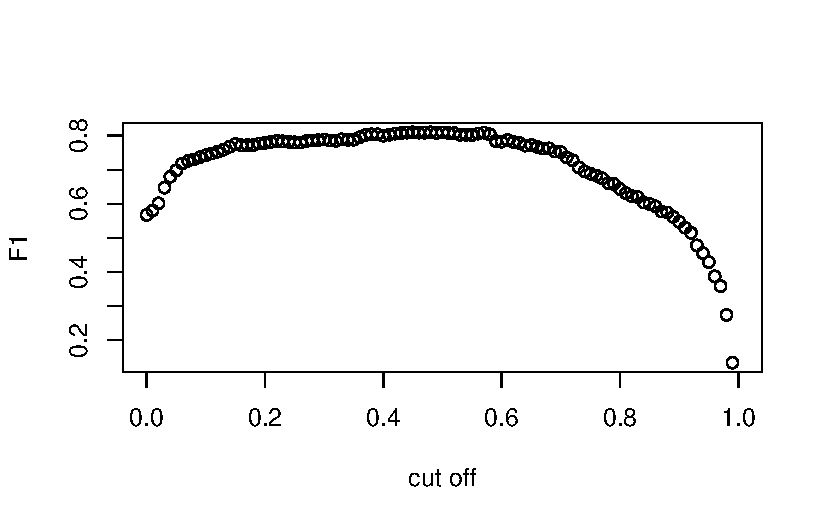
\includegraphics{FinalProject_files/figure-pdf/unnamed-chunk-26-1.pdf}

\begin{Shaded}
\begin{Highlighting}[]
\NormalTok{optimal.cutoff }\OtherTok{=}\NormalTok{ test\_cutoff[}\FunctionTok{which.max}\NormalTok{(test\_cutoff[,}\DecValTok{8}\NormalTok{]),]}
\NormalTok{optimal.cutoff[}\DecValTok{1}\NormalTok{]}
\end{Highlighting}
\end{Shaded}

\begin{verbatim}
  p 
0.5 
\end{verbatim}

\begin{Shaded}
\begin{Highlighting}[]
\NormalTok{observations.train }\OtherTok{=}\NormalTok{ train}\SpecialCharTok{$}\NormalTok{survived}
\NormalTok{observations.test }\OtherTok{=}\NormalTok{ test}\SpecialCharTok{$}\NormalTok{survived}

\CommentTok{\# Confusion matrix on base log model on train data}
\NormalTok{y\_hat\_prob }\OtherTok{=} \FunctionTok{predict}\NormalTok{(lmod, train, }\AttributeTok{type=}\StringTok{"response"}\NormalTok{)}
\NormalTok{predictions.binary.model.train }\OtherTok{\textless{}{-}} \FunctionTok{ifelse}\NormalTok{(y\_hat\_prob }\SpecialCharTok{\textgreater{}}\NormalTok{ optimal.cutoff[}\DecValTok{1}\NormalTok{], }\DecValTok{1}\NormalTok{, }\DecValTok{0}\NormalTok{)}
\NormalTok{confusion.matrix.binary.model.train }\OtherTok{\textless{}{-}} \FunctionTok{confusionMatrix}\NormalTok{(}\FunctionTok{as.factor}\NormalTok{(predictions.binary.model.train),}\FunctionTok{as.factor}\NormalTok{(observations.train),}\AttributeTok{mode=}\StringTok{"prec\_recall"}\NormalTok{, }\AttributeTok{positive =} \StringTok{"1"}\NormalTok{)}
\NormalTok{base.model.accuracy }\OtherTok{=}\NormalTok{ confusion.matrix.binary.model.train}\SpecialCharTok{$}\NormalTok{overall[}\StringTok{\textquotesingle{}Accuracy\textquotesingle{}}\NormalTok{]}
\NormalTok{base.model.f1 }\OtherTok{=}\NormalTok{ confusion.matrix.binary.model.train}\SpecialCharTok{$}\NormalTok{byClass[}\StringTok{\textquotesingle{}F1\textquotesingle{}}\NormalTok{]}
\NormalTok{base.model.train.summary }\OtherTok{=} \FunctionTok{data.frame}\NormalTok{(}
  \AttributeTok{Accuracy =}\NormalTok{ base.model.accuracy,}
  \AttributeTok{F1 =}\NormalTok{ base.model.f1}
\NormalTok{)}
\FunctionTok{row.names}\NormalTok{(base.model.train.summary) }\OtherTok{\textless{}{-}} \StringTok{\textquotesingle{}base.model.train\textquotesingle{}}

\CommentTok{\# Confusion matrix on base log model on test data}
\NormalTok{y\_hat\_prob }\OtherTok{=} \FunctionTok{predict}\NormalTok{(lmod, test, }\AttributeTok{type=}\StringTok{"response"}\NormalTok{)}

\NormalTok{predictions.binary.model.test }\OtherTok{\textless{}{-}} \FunctionTok{ifelse}\NormalTok{(y\_hat\_prob }\SpecialCharTok{\textgreater{}}\NormalTok{ optimal.cutoff[}\DecValTok{1}\NormalTok{], }\DecValTok{1}\NormalTok{, }\DecValTok{0}\NormalTok{)}

\NormalTok{confusion.matrix.binary.model.test }\OtherTok{\textless{}{-}} \FunctionTok{confusionMatrix}\NormalTok{(}\FunctionTok{as.factor}\NormalTok{(predictions.binary.model.test),}\FunctionTok{as.factor}\NormalTok{(observations.test), }\AttributeTok{positive =} \StringTok{"1"}\NormalTok{)}

\NormalTok{base.model.accuracy.test }\OtherTok{=}\NormalTok{ confusion.matrix.binary.model.test}\SpecialCharTok{$}\NormalTok{overall[}\StringTok{\textquotesingle{}Accuracy\textquotesingle{}}\NormalTok{]}
\NormalTok{base.model.f1.test }\OtherTok{=}\NormalTok{ confusion.matrix.binary.model.test}\SpecialCharTok{$}\NormalTok{byClass[}\StringTok{\textquotesingle{}F1\textquotesingle{}}\NormalTok{]}

\NormalTok{base.model.test.summary }\OtherTok{=} \FunctionTok{data.frame}\NormalTok{(}
  \AttributeTok{Accuracy =}\NormalTok{ base.model.accuracy.test,}
  \AttributeTok{F1 =}\NormalTok{ base.model.f1.test}
\NormalTok{)}
\FunctionTok{row.names}\NormalTok{(base.model.test.summary) }\OtherTok{\textless{}{-}} \StringTok{\textquotesingle{}base.model.test\textquotesingle{}}

\CommentTok{\# Confusion matrix on stepwise log model on train data}
\NormalTok{y\_hat\_prob }\OtherTok{=} \FunctionTok{predict}\NormalTok{(binary.model.stepwise, train, }\AttributeTok{type=}\StringTok{"response"}\NormalTok{)}
\NormalTok{predictions.binary.model.step.train }\OtherTok{\textless{}{-}} \FunctionTok{ifelse}\NormalTok{(y\_hat\_prob }\SpecialCharTok{\textgreater{}}\NormalTok{ optimal.cutoff[}\DecValTok{1}\NormalTok{], }\DecValTok{1}\NormalTok{, }\DecValTok{0}\NormalTok{)}
\NormalTok{confusion.matrix.binary.model.step.train }\OtherTok{\textless{}{-}} \FunctionTok{confusionMatrix}\NormalTok{(}\FunctionTok{as.factor}\NormalTok{(predictions.binary.model.step.train),}\FunctionTok{as.factor}\NormalTok{(observations.train),}\AttributeTok{mode=}\StringTok{"prec\_recall"}\NormalTok{, }\AttributeTok{positive =} \StringTok{"1"}\NormalTok{)}
\NormalTok{stepwise.model.accuracy }\OtherTok{=}\NormalTok{ confusion.matrix.binary.model.step.train}\SpecialCharTok{$}\NormalTok{overall[}\StringTok{\textquotesingle{}Accuracy\textquotesingle{}}\NormalTok{]}
\NormalTok{stepwise.model.f1 }\OtherTok{=}\NormalTok{ confusion.matrix.binary.model.step.train}\SpecialCharTok{$}\NormalTok{byClass[}\StringTok{\textquotesingle{}F1\textquotesingle{}}\NormalTok{]}
\NormalTok{stepwise.model.train.summary }\OtherTok{=} \FunctionTok{data.frame}\NormalTok{(}
  \AttributeTok{Accuracy =}\NormalTok{ stepwise.model.accuracy,}
  \AttributeTok{F1 =}\NormalTok{ stepwise.model.f1}
\NormalTok{)}
\FunctionTok{row.names}\NormalTok{(stepwise.model.train.summary) }\OtherTok{\textless{}{-}} \StringTok{\textquotesingle{}stepwise.model.train\textquotesingle{}}

\CommentTok{\# Confusion matrix on stepwise log model on test data}
\NormalTok{y\_hat\_prob }\OtherTok{=} \FunctionTok{predict}\NormalTok{(binary.model.stepwise, test, }\AttributeTok{type=}\StringTok{"response"}\NormalTok{)}
\NormalTok{predictions.binary.model.step.test }\OtherTok{\textless{}{-}} \FunctionTok{ifelse}\NormalTok{(y\_hat\_prob }\SpecialCharTok{\textgreater{}}\NormalTok{ optimal.cutoff[}\DecValTok{1}\NormalTok{], }\DecValTok{1}\NormalTok{, }\DecValTok{0}\NormalTok{)}
\NormalTok{confusion.matrix.binary.model.step.test }\OtherTok{\textless{}{-}} \FunctionTok{confusionMatrix}\NormalTok{(}\FunctionTok{as.factor}\NormalTok{(predictions.binary.model.step.test),}\FunctionTok{as.factor}\NormalTok{(observations.test),}\AttributeTok{mode=}\StringTok{"prec\_recall"}\NormalTok{, }\AttributeTok{positive =} \StringTok{"1"}\NormalTok{)}
\NormalTok{stepwise.model.accuracy }\OtherTok{=}\NormalTok{ confusion.matrix.binary.model.step.test}\SpecialCharTok{$}\NormalTok{overall[}\StringTok{\textquotesingle{}Accuracy\textquotesingle{}}\NormalTok{]}
\NormalTok{stepwise.model.f1 }\OtherTok{=}\NormalTok{ confusion.matrix.binary.model.step.test}\SpecialCharTok{$}\NormalTok{byClass[}\StringTok{\textquotesingle{}F1\textquotesingle{}}\NormalTok{]}
\NormalTok{stepwise.model.test.summary }\OtherTok{=} \FunctionTok{data.frame}\NormalTok{(}
  \AttributeTok{Accuracy =}\NormalTok{ stepwise.model.accuracy,}
  \AttributeTok{F1 =}\NormalTok{ stepwise.model.f1}
\NormalTok{)}
\FunctionTok{row.names}\NormalTok{(stepwise.model.test.summary) }\OtherTok{\textless{}{-}} \StringTok{\textquotesingle{}stepwise.model.test\textquotesingle{}}

\CommentTok{\# Confusion matrix on log model w/ insig. pred. removed}
\NormalTok{y\_hat\_prob }\OtherTok{=} \FunctionTok{predict}\NormalTok{(binary.model.filtered, train, }\AttributeTok{type=}\StringTok{"response"}\NormalTok{)}
\NormalTok{predictions.binary.model.filtered.train }\OtherTok{\textless{}{-}} \FunctionTok{ifelse}\NormalTok{(y\_hat\_prob }\SpecialCharTok{\textgreater{}}\NormalTok{ optimal.cutoff[}\DecValTok{1}\NormalTok{], }\DecValTok{1}\NormalTok{, }\DecValTok{0}\NormalTok{)}
\NormalTok{confusion.matrix.binary.model.filtered.train }\OtherTok{\textless{}{-}} \FunctionTok{confusionMatrix}\NormalTok{(}\FunctionTok{as.factor}\NormalTok{(predictions.binary.model.filtered.train),}\FunctionTok{as.factor}\NormalTok{(observations.train),}\AttributeTok{mode=}\StringTok{"prec\_recall"}\NormalTok{, }\AttributeTok{positive =} \StringTok{"1"}\NormalTok{)}
\NormalTok{filtered.model.accuracy }\OtherTok{=}\NormalTok{ confusion.matrix.binary.model.filtered.train}\SpecialCharTok{$}\NormalTok{overall[}\StringTok{\textquotesingle{}Accuracy\textquotesingle{}}\NormalTok{]}
\NormalTok{filtered.model.f1 }\OtherTok{=}\NormalTok{ confusion.matrix.binary.model.filtered.train}\SpecialCharTok{$}\NormalTok{byClass[}\StringTok{\textquotesingle{}F1\textquotesingle{}}\NormalTok{]}
\NormalTok{filtered.model.train.summary }\OtherTok{=} \FunctionTok{data.frame}\NormalTok{(}
  \AttributeTok{Accuracy =}\NormalTok{ filtered.model.accuracy,}
  \AttributeTok{F1 =}\NormalTok{ filtered.model.f1}
\NormalTok{)}
\FunctionTok{row.names}\NormalTok{(filtered.model.train.summary) }\OtherTok{\textless{}{-}} \StringTok{\textquotesingle{}filtered.model.train\textquotesingle{}}

\CommentTok{\# Confusion matrix on log model w/ insig. pred. removed}
\NormalTok{y\_hat\_prob }\OtherTok{=} \FunctionTok{predict}\NormalTok{(binary.model.filtered, test, }\AttributeTok{type=}\StringTok{"response"}\NormalTok{)}

\NormalTok{predictions.binary.model.filtered.test }\OtherTok{\textless{}{-}} \FunctionTok{ifelse}\NormalTok{(y\_hat\_prob }\SpecialCharTok{\textgreater{}}\NormalTok{ optimal.cutoff[}\DecValTok{1}\NormalTok{], }\DecValTok{1}\NormalTok{, }\DecValTok{0}\NormalTok{)}

\NormalTok{confusion.matrix.binary.model.filtered.test }\OtherTok{\textless{}{-}} \FunctionTok{confusionMatrix}\NormalTok{(}\FunctionTok{as.factor}\NormalTok{(predictions.binary.model.filtered.test),}\FunctionTok{as.factor}\NormalTok{(observations.test),}\AttributeTok{mode=}\StringTok{"prec\_recall"}\NormalTok{, }\AttributeTok{positive =} \StringTok{"1"}\NormalTok{)}

\NormalTok{filtered.model.accuracy }\OtherTok{=}\NormalTok{ confusion.matrix.binary.model.filtered.test}\SpecialCharTok{$}\NormalTok{overall[}\StringTok{\textquotesingle{}Accuracy\textquotesingle{}}\NormalTok{]}
\NormalTok{filtered.model.f1 }\OtherTok{=}\NormalTok{ confusion.matrix.binary.model.filtered.test}\SpecialCharTok{$}\NormalTok{byClass[}\StringTok{\textquotesingle{}F1\textquotesingle{}}\NormalTok{]}

\NormalTok{filtered.model.test.summary }\OtherTok{=} \FunctionTok{data.frame}\NormalTok{(}
  \AttributeTok{Accuracy =}\NormalTok{ filtered.model.accuracy,}
  \AttributeTok{F1 =}\NormalTok{ filtered.model.f1}
\NormalTok{)}
\FunctionTok{row.names}\NormalTok{(filtered.model.test.summary) }\OtherTok{\textless{}{-}} \StringTok{\textquotesingle{}filtered.model.test\textquotesingle{}}

\CommentTok{\# Confusion matrix on log model w/ high vif pred. removed}
\NormalTok{y\_hat\_prob }\OtherTok{=} \FunctionTok{predict}\NormalTok{(vif.model, train, }\AttributeTok{type=}\StringTok{"response"}\NormalTok{)}
\NormalTok{predictions.binary.model.vif.train }\OtherTok{\textless{}{-}} \FunctionTok{ifelse}\NormalTok{(y\_hat\_prob }\SpecialCharTok{\textgreater{}}\NormalTok{ optimal.cutoff[}\DecValTok{1}\NormalTok{], }\DecValTok{1}\NormalTok{, }\DecValTok{0}\NormalTok{)}
\NormalTok{confusion.matrix.binary.model.vif.train }\OtherTok{\textless{}{-}} \FunctionTok{confusionMatrix}\NormalTok{(}\FunctionTok{as.factor}\NormalTok{(predictions.binary.model.vif.train),}\FunctionTok{as.factor}\NormalTok{(observations.train),}\AttributeTok{mode=}\StringTok{"prec\_recall"}\NormalTok{, }\AttributeTok{positive =} \StringTok{"1"}\NormalTok{)}
\NormalTok{vif.model.accuracy }\OtherTok{=}\NormalTok{ confusion.matrix.binary.model.vif.train}\SpecialCharTok{$}\NormalTok{overall[}\StringTok{\textquotesingle{}Accuracy\textquotesingle{}}\NormalTok{]}
\NormalTok{vif.model.f1 }\OtherTok{=}\NormalTok{ confusion.matrix.binary.model.vif.train}\SpecialCharTok{$}\NormalTok{byClass[}\StringTok{\textquotesingle{}F1\textquotesingle{}}\NormalTok{]}
\NormalTok{vif.model.train.summary }\OtherTok{=} \FunctionTok{data.frame}\NormalTok{(}
  \AttributeTok{Accuracy =}\NormalTok{ vif.model.accuracy,}
  \AttributeTok{F1 =}\NormalTok{ vif.model.f1}
\NormalTok{)}
\FunctionTok{row.names}\NormalTok{(vif.model.train.summary) }\OtherTok{\textless{}{-}} \StringTok{\textquotesingle{}vif.model.train\textquotesingle{}}

\CommentTok{\# Confusion matrix on log model w/ high vif pred. removed}
\NormalTok{y\_hat\_prob }\OtherTok{=} \FunctionTok{predict}\NormalTok{(vif.model, test, }\AttributeTok{type=}\StringTok{"response"}\NormalTok{)}
\NormalTok{predictions.binary.model.vif.test }\OtherTok{\textless{}{-}} \FunctionTok{ifelse}\NormalTok{(y\_hat\_prob }\SpecialCharTok{\textgreater{}}\NormalTok{ optimal.cutoff[}\DecValTok{1}\NormalTok{], }\DecValTok{1}\NormalTok{, }\DecValTok{0}\NormalTok{)}
\NormalTok{confusion.matrix.binary.model.vif.test }\OtherTok{\textless{}{-}} \FunctionTok{confusionMatrix}\NormalTok{(}\FunctionTok{as.factor}\NormalTok{(predictions.binary.model.vif.test),}\FunctionTok{as.factor}\NormalTok{(observations.test),}\AttributeTok{mode=}\StringTok{"prec\_recall"}\NormalTok{, }\AttributeTok{positive =} \StringTok{"1"}\NormalTok{)}
\NormalTok{vif.model.accuracy }\OtherTok{=}\NormalTok{ confusion.matrix.binary.model.vif.test}\SpecialCharTok{$}\NormalTok{overall[}\StringTok{\textquotesingle{}Accuracy\textquotesingle{}}\NormalTok{]}
\NormalTok{vif.model.f1 }\OtherTok{=}\NormalTok{ confusion.matrix.binary.model.vif.test}\SpecialCharTok{$}\NormalTok{byClass[}\StringTok{\textquotesingle{}F1\textquotesingle{}}\NormalTok{]}
\NormalTok{vif.model.test.summary }\OtherTok{=} \FunctionTok{data.frame}\NormalTok{(}
  \AttributeTok{Accuracy =}\NormalTok{ vif.model.accuracy,}
  \AttributeTok{F1 =}\NormalTok{ vif.model.f1}
\NormalTok{)}
\FunctionTok{row.names}\NormalTok{(vif.model.test.summary) }\OtherTok{\textless{}{-}} \StringTok{\textquotesingle{}vif.model.test\textquotesingle{}}
\end{Highlighting}
\end{Shaded}

\begin{Shaded}
\begin{Highlighting}[]
\FunctionTok{data.frame}\NormalTok{(}\FunctionTok{rbind}\NormalTok{(base.model.train.summary, base.model.test.summary, }
\NormalTok{                 stepwise.model.train.summary, stepwise.model.test.summary,}
\NormalTok{                 filtered.model.train.summary, filtered.model.test.summary,}
\NormalTok{                 vif.model.train.summary,vif.model.test.summary))}
\end{Highlighting}
\end{Shaded}

\begin{longtable}[]{@{}lrr@{}}
\caption{Comparison of all log models performance}\tabularnewline
\toprule\noalign{}
& Accuracy & F1 \\
\midrule\noalign{}
\endfirsthead
\toprule\noalign{}
& Accuracy & F1 \\
\midrule\noalign{}
\endhead
\bottomrule\noalign{}
\endlastfoot
base.model.train & 0.8504367 & 0.8115543 \\
base.model.test & 0.8392857 & 0.7758007 \\
stepwise.model.train & 0.8231441 & 0.7692308 \\
stepwise.model.test & 0.8367347 & 0.7611940 \\
filtered.model.train & 0.8504367 & 0.8115543 \\
filtered.model.test & 0.8418367 & 0.7801418 \\
vif.model.train & 0.8351528 & 0.7911480 \\
vif.model.test & 0.8392857 & 0.7789474 \\
\end{longtable}

\section{Challenger Models}\label{challenger-models}

We decided to build a Poisson model for our challenger model. After
building our original poisson model, we first check to see if the
variables are important.

Ho: Variables are not important

Ha: Variable are important

Since we have a p-value of 0, we reject the null hypothesis. Variables
are important.

Our poisson model has three significant variables, pclass\_2, sex\_M,
and deck\_F with an alpha of 0.05.

According to the poisson regression:

The odds of survival increases by 37.6\% when the passenger is second
class. ((exp(0.31918) - 1) * 100)

The odds of survival decreases by 68.14\% when the passenger is male.
((exp(-1.144) - 1) * 100)

The odds of survival decreases by 64.76\% when the passenger is from
deck G. ((exp(-1.043) - 1) * 100)

Our Poisson Regression has an accuracy of 74.74\% with optimal
cutoff(.17) based on max F1 score (0.71954).

\begin{Shaded}
\begin{Highlighting}[]
\FunctionTok{library}\NormalTok{(MASS)}

\CommentTok{\# Train base Poisson model:}
\NormalTok{poissonReg\_full }\OtherTok{\textless{}{-}} \FunctionTok{glm}\NormalTok{(survived }\SpecialCharTok{\textasciitilde{}}\NormalTok{ .,}\AttributeTok{family=}\NormalTok{poisson, train)}

\CommentTok{\# compare the fitted model to the null model and calculate if the variables are important}
\FunctionTok{summary}\NormalTok{(poissonReg\_full)}
\end{Highlighting}
\end{Shaded}

\begin{verbatim}

Call:
glm(formula = survived ~ ., family = poisson, data = train)

Coefficients:
              Estimate Std. Error z value Pr(>|z|)    
(Intercept)  7.787e-01  3.449e-01   2.258 0.023946 *  
age         -1.609e-02  4.355e-03  -3.695 0.000220 ***
sibsp       -6.954e-02  6.979e-02  -0.996 0.319019    
parch       -5.055e-04  6.756e-02  -0.007 0.994030    
fare         9.289e-05  1.025e-03   0.091 0.927778    
pclass_1     3.590e-01  2.047e-01   1.753 0.079536 .  
pclass_2     5.102e-01  1.532e-01   3.329 0.000871 ***
sex_M       -1.095e+00  1.201e-01  -9.112  < 2e-16 ***
embarked_C   1.072e-01  1.349e-01   0.795 0.426660    
embarked_Q   4.537e-01  2.162e-01   2.098 0.035872 *  
deck_A      -6.157e-01  4.732e-01  -1.301 0.193282    
deck_B      -6.494e-01  4.130e-01  -1.572 0.115868    
deck_C      -6.891e-01  3.943e-01  -1.748 0.080527 .  
deck_D      -7.195e-01  3.962e-01  -1.816 0.069347 .  
deck_E      -2.300e-01  3.556e-01  -0.647 0.517786    
deck_F      -1.527e+00  3.419e-01  -4.467 7.94e-06 ***
---
Signif. codes:  0 '***' 0.001 '**' 0.01 '*' 0.05 '.' 0.1 ' ' 1

(Dispersion parameter for poisson family taken to be 1)

    Null deviance: 672.00  on 915  degrees of freedom
Residual deviance: 404.15  on 900  degrees of freedom
AIC: 1162.2

Number of Fisher Scoring iterations: 5
\end{verbatim}

\begin{Shaded}
\begin{Highlighting}[]
\DecValTok{1}\SpecialCharTok{{-}}\FunctionTok{pchisq}\NormalTok{(}\FloatTok{672.00{-}409.95}\NormalTok{, }\FunctionTok{length}\NormalTok{(}\FunctionTok{coef}\NormalTok{(poissonReg\_full)) }\SpecialCharTok{{-}} \DecValTok{1}\NormalTok{)}
\end{Highlighting}
\end{Shaded}

\begin{verbatim}
[1] 0
\end{verbatim}

\begin{Shaded}
\begin{Highlighting}[]
\CommentTok{\# We then reduce the model and see if the removed variables are significant}
\NormalTok{poissonReg\_reduced }\OtherTok{\textless{}{-}} \FunctionTok{glm}\NormalTok{(survived }\SpecialCharTok{\textasciitilde{}}\NormalTok{ pclass\_2}\SpecialCharTok{+}\NormalTok{sex\_M}\SpecialCharTok{+}\NormalTok{deck\_F,}\AttributeTok{family=}\NormalTok{poisson, train)}

\CommentTok{\# Verify that all variables are significant and no more can be dropped}
\FunctionTok{anova}\NormalTok{(poissonReg\_reduced, poissonReg\_full, }\AttributeTok{test=}\StringTok{"Chi"}\NormalTok{)}
\end{Highlighting}
\end{Shaded}

\begin{longtable}[]{@{}rrrrr@{}}
\toprule\noalign{}
Resid. Df & Resid. Dev & Df & Deviance & Pr(\textgreater Chi) \\
\midrule\noalign{}
\endhead
\bottomrule\noalign{}
\endlastfoot
912 & 430.4971 & NA & NA & NA \\
900 & 404.1538 & 12 & 26.34334 & 0.0095947 \\
\end{longtable}

\begin{Shaded}
\begin{Highlighting}[]
\FunctionTok{drop1}\NormalTok{(poissonReg\_reduced,}\AttributeTok{test=}\StringTok{"Chi"}\NormalTok{)}
\end{Highlighting}
\end{Shaded}

\begin{longtable}[]{@{}lrrrrr@{}}
\toprule\noalign{}
& Df & Deviance & AIC & LRT & Pr(\textgreater Chi) \\
\midrule\noalign{}
\endhead
\bottomrule\noalign{}
\endlastfoot
& NA & 430.4971 & 1164.497 & NA & NA \\
pclass\_2 & 1 & 436.9472 & 1168.947 & 6.450073 & 0.0110948 \\
sex\_M & 1 & 540.1126 & 1272.113 & 109.615481 & 0.0000000 \\
deck\_F & 1 & 520.5287 & 1252.529 & 90.031585 & 0.0000000 \\
\end{longtable}

\begin{Shaded}
\begin{Highlighting}[]
\DocumentationTok{\#\#\# Train Data}

\CommentTok{\# Testing against train data}
\NormalTok{predicted\_probs }\OtherTok{\textless{}{-}} \FunctionTok{predict}\NormalTok{(poissonReg\_reduced, }\AttributeTok{newdata =}\NormalTok{ train, }\AttributeTok{type =} \StringTok{"response"}\NormalTok{)}

\CommentTok{\# Get the results of different cutoff values}
\NormalTok{trainResult}\OtherTok{\textless{}{-}}\FunctionTok{cutoff.prg}\NormalTok{(predicted\_probs,train}\SpecialCharTok{$}\NormalTok{survived)}
\end{Highlighting}
\end{Shaded}

\begin{verbatim}
Warning in confusionMatrix.default(as.factor(predictions), as.factor(act), :
Levels are not in the same order for reference and data. Refactoring data to
match.
Warning in confusionMatrix.default(as.factor(predictions), as.factor(act), :
Levels are not in the same order for reference and data. Refactoring data to
match.
Warning in confusionMatrix.default(as.factor(predictions), as.factor(act), :
Levels are not in the same order for reference and data. Refactoring data to
match.
Warning in confusionMatrix.default(as.factor(predictions), as.factor(act), :
Levels are not in the same order for reference and data. Refactoring data to
match.
Warning in confusionMatrix.default(as.factor(predictions), as.factor(act), :
Levels are not in the same order for reference and data. Refactoring data to
match.
Warning in confusionMatrix.default(as.factor(predictions), as.factor(act), :
Levels are not in the same order for reference and data. Refactoring data to
match.
Warning in confusionMatrix.default(as.factor(predictions), as.factor(act), :
Levels are not in the same order for reference and data. Refactoring data to
match.
Warning in confusionMatrix.default(as.factor(predictions), as.factor(act), :
Levels are not in the same order for reference and data. Refactoring data to
match.
Warning in confusionMatrix.default(as.factor(predictions), as.factor(act), :
Levels are not in the same order for reference and data. Refactoring data to
match.
Warning in confusionMatrix.default(as.factor(predictions), as.factor(act), :
Levels are not in the same order for reference and data. Refactoring data to
match.
Warning in confusionMatrix.default(as.factor(predictions), as.factor(act), :
Levels are not in the same order for reference and data. Refactoring data to
match.
Warning in confusionMatrix.default(as.factor(predictions), as.factor(act), :
Levels are not in the same order for reference and data. Refactoring data to
match.
\end{verbatim}

\begin{Shaded}
\begin{Highlighting}[]
\CommentTok{\# We get get the optimal p cut off value based on the maximum F1 score}
\FunctionTok{plot}\NormalTok{(trainResult[,}\DecValTok{1}\NormalTok{],trainResult[,}\DecValTok{8}\NormalTok{],}\AttributeTok{xlab=}\StringTok{"cut off"}\NormalTok{,}\AttributeTok{ylab=}\StringTok{"F1"}\NormalTok{)}
\end{Highlighting}
\end{Shaded}

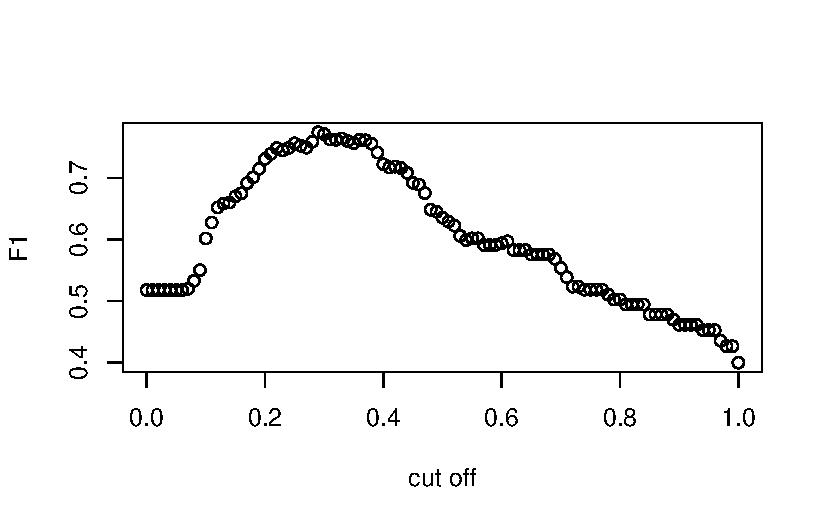
\includegraphics{FinalProject_files/figure-pdf/poisson-1.pdf}

\begin{Shaded}
\begin{Highlighting}[]
\NormalTok{poisson.model.cutoff }\OtherTok{=}\NormalTok{ trainResult[}\FunctionTok{which.max}\NormalTok{(trainResult[,}\DecValTok{8}\NormalTok{]),]}

\CommentTok{\# Get the F1 and Accuracy for train data using the optimal p value}
\NormalTok{observations.train }\OtherTok{\textless{}{-}}\NormalTok{ train}\SpecialCharTok{$}\NormalTok{survived}
\NormalTok{predictions.poisson.model.train }\OtherTok{\textless{}{-}} \FunctionTok{ifelse}\NormalTok{(predicted\_probs }\SpecialCharTok{\textgreater{}}\NormalTok{ poisson.model.cutoff[}\DecValTok{1}\NormalTok{], }\DecValTok{1}\NormalTok{, }\DecValTok{0}\NormalTok{)}

\NormalTok{confusion.matrix.binary.model.poisson.train }\OtherTok{\textless{}{-}} \FunctionTok{confusionMatrix}\NormalTok{(}\FunctionTok{as.factor}\NormalTok{(predictions.poisson.model.train),}\FunctionTok{as.factor}\NormalTok{(observations.train), }\AttributeTok{positive =} \StringTok{"1"}\NormalTok{)}

\NormalTok{poisson.model.accuracy.train }\OtherTok{=}\NormalTok{ confusion.matrix.binary.model.poisson.train}\SpecialCharTok{$}\NormalTok{overall[}\StringTok{\textquotesingle{}Accuracy\textquotesingle{}}\NormalTok{]}
\NormalTok{poisson.model.f1.train }\OtherTok{=}\NormalTok{ confusion.matrix.binary.model.poisson.train}\SpecialCharTok{$}\NormalTok{byClass[}\StringTok{\textquotesingle{}F1\textquotesingle{}}\NormalTok{]}

\NormalTok{poisson.model.train.summary }\OtherTok{=} \FunctionTok{data.frame}\NormalTok{(}
  \AttributeTok{Accuracy =}\NormalTok{ poisson.model.accuracy.train,}
  \AttributeTok{F1 =}\NormalTok{ poisson.model.f1.train}
\NormalTok{)}

\FunctionTok{row.names}\NormalTok{(poisson.model.train.summary) }\OtherTok{\textless{}{-}} \StringTok{\textquotesingle{}poisson.model.train\textquotesingle{}}

\DocumentationTok{\#\#\# Test Data}

\CommentTok{\# Testing against test data}
\NormalTok{predicted\_probs }\OtherTok{\textless{}{-}} \FunctionTok{predict}\NormalTok{(poissonReg\_reduced, }\AttributeTok{newdata =}\NormalTok{ test, }\AttributeTok{type =} \StringTok{"response"}\NormalTok{)}

\CommentTok{\# Get the F1 and Accuracy for test data using the optimal p value}
\NormalTok{observations.test }\OtherTok{\textless{}{-}}\NormalTok{ test}\SpecialCharTok{$}\NormalTok{survived}
\NormalTok{predictions.poisson.model.test }\OtherTok{\textless{}{-}} \FunctionTok{ifelse}\NormalTok{(predicted\_probs }\SpecialCharTok{\textgreater{}}\NormalTok{ poisson.model.cutoff[}\DecValTok{1}\NormalTok{], }\DecValTok{1}\NormalTok{, }\DecValTok{0}\NormalTok{)}

\NormalTok{confusion.matrix.binary.model.poisson.test }\OtherTok{\textless{}{-}} \FunctionTok{confusionMatrix}\NormalTok{(}\FunctionTok{as.factor}\NormalTok{(predictions.poisson.model.test),}\FunctionTok{as.factor}\NormalTok{(observations.test), }\AttributeTok{positive =} \StringTok{"1"}\NormalTok{)}

\NormalTok{poisson.model.accuracy.test }\OtherTok{=}\NormalTok{ confusion.matrix.binary.model.poisson.test}\SpecialCharTok{$}\NormalTok{overall[}\StringTok{\textquotesingle{}Accuracy\textquotesingle{}}\NormalTok{]}
\NormalTok{poisson.model.f1.test }\OtherTok{=}\NormalTok{ confusion.matrix.binary.model.poisson.test}\SpecialCharTok{$}\NormalTok{byClass[}\StringTok{\textquotesingle{}F1\textquotesingle{}}\NormalTok{]}

\NormalTok{poisson.model.test.summary }\OtherTok{=} \FunctionTok{data.frame}\NormalTok{(}
  \AttributeTok{Accuracy =}\NormalTok{ poisson.model.accuracy.test,}
  \AttributeTok{F1 =}\NormalTok{ poisson.model.f1.test}
\NormalTok{)}

\FunctionTok{row.names}\NormalTok{(poisson.model.test.summary) }\OtherTok{\textless{}{-}} \StringTok{\textquotesingle{}poisson.model.test\textquotesingle{}}

\FunctionTok{data.frame}\NormalTok{(}\FunctionTok{rbind}\NormalTok{(poisson.model.train.summary,poisson.model.test.summary ))}
\end{Highlighting}
\end{Shaded}

\begin{longtable}[]{@{}lrr@{}}
\toprule\noalign{}
& Accuracy & F1 \\
\midrule\noalign{}
\endhead
\bottomrule\noalign{}
\endlastfoot
poisson.model.train & 0.7663755 & 0.7590090 \\
poisson.model.test & 0.7474490 & 0.7195467 \\
\end{longtable}

\section{Model Limitation and
Assumptions}\label{model-limitation-and-assumptions}

The champion model selected is the filtered logistic regression model
due to its superior test accuracy (84.1\%) and F1 score (0.78014). The
filtered logistic regression model was developed through backward
elimination procedure, applied to the full base model. This process
iteratively removed predictors with high p-values until only
statistically significant predictors remained. The base model is used as
the benchmark due to its similar performance and broader feature set.

\begin{Shaded}
\begin{Highlighting}[]
\FunctionTok{summary}\NormalTok{(binary.model.filtered)}
\end{Highlighting}
\end{Shaded}

\begin{verbatim}

Call:
glm(formula = survived ~ age + sibsp + pclass_1 + pclass_2 + 
    sex_M + embarked_C + embarked_Q + deck_A + deck_B + deck_C + 
    deck_D + deck_F, family = binomial, data = train)

Coefficients:
             Estimate Std. Error z value Pr(>|z|)    
(Intercept)  5.745434   0.507728  11.316  < 2e-16 ***
age         -0.053296   0.008919  -5.976 2.29e-09 ***
sibsp       -0.254771   0.116064  -2.195  0.02816 *  
pclass_1     0.799195   0.449070   1.780  0.07513 .  
pclass_2     1.827594   0.297584   6.141 8.18e-10 ***
sex_M       -3.278525   0.251332 -13.045  < 2e-16 ***
embarked_C   0.830036   0.282806   2.935  0.00334 ** 
embarked_Q   0.785344   0.354744   2.214  0.02684 *  
deck_A      -2.549579   0.616634  -4.135 3.55e-05 ***
deck_B      -1.896873   0.585234  -3.241  0.00119 ** 
deck_C      -2.032446   0.516558  -3.935 8.33e-05 ***
deck_D      -2.995951   0.494319  -6.061 1.35e-09 ***
deck_F      -4.706551   0.404816 -11.626  < 2e-16 ***
---
Signif. codes:  0 '***' 0.001 '**' 0.01 '*' 0.05 '.' 0.1 ' ' 1

(Dispersion parameter for binomial family taken to be 1)

    Null deviance: 1230.1  on 915  degrees of freedom
Residual deviance:  635.0  on 903  degrees of freedom
AIC: 661

Number of Fisher Scoring iterations: 6
\end{verbatim}

To further evaluate and benchmark the logistic regression models, we
computed RMSE, R², and MAE using the predicted probabilities against the
actual binary outcomes. While traditional R² is not appropriate for
logistic models, these metrics provide insight into how well the
predicted probabilities align with observed outcomes. The Filtered model
appears to have higher R² (0.4425\textgreater0.4342), lower RMSE(0.3945
\textless{} 0.3977) and MAE (0.1556 \textless0.1582). Additionally,
model validation was done through train/test split with consistent
performance across sets. The performance on test data and train data
show minimal difference, indicating the model is robust, no over-itting
problem.

To evaluate the stability and fit of the base and filtered logistic
regression models, we conducted residual-based tests on their linear
analogs. While logistic regression does not formally require normally
distributed or homoscedastic residuals, these tests offer insights into
model specification quality and residual behavior.

Breusch-Pagan Test: Both models exhibit statistically significant
heteroskedasticity (p \textless{} 0.01)

Shapiro-Wilk Test: Both models show highly significant deviations from
normality (p \textless{} 0.01)

Both models show similar residual behavior, with slight
heteroskedasticity and non-normality. These findings do not violate
logistic regression assumptions but suggest the model could be further
improved through additional transformations or interaction terms.

Multicollinearity was significantly lower in the filtered model (max
VIF: 3.69 vs.~16.63), supporting better generalization and
interpretability.

\begin{Shaded}
\begin{Highlighting}[]
\FunctionTok{library}\NormalTok{(car)}

\CommentTok{\# Normality Test}
\CommentTok{\# Breusch Pagan Test on Logistic Model}
\NormalTok{BPtest\_basemodel }\OtherTok{\textless{}{-}} \FunctionTok{ols\_test\_breusch\_pagan}\NormalTok{(lmod)}
\NormalTok{BPtest\_filtered.model }\OtherTok{\textless{}{-}} \FunctionTok{ols\_test\_breusch\_pagan}\NormalTok{(binary.model.filtered)}

\CommentTok{\# Shapiro{-}Wilk test}
\NormalTok{SWtest\_basemodel }\OtherTok{\textless{}{-}} \FunctionTok{shapiro.test}\NormalTok{(}\FunctionTok{residuals}\NormalTok{(lmod))}
\NormalTok{SWtest\_filteredmodel }\OtherTok{\textless{}{-}} \FunctionTok{shapiro.test}\NormalTok{(}\FunctionTok{residuals}\NormalTok{(binary.model.filtered))}


\CommentTok{\# Combine into unified rows}
\NormalTok{diagnostics\_summary }\OtherTok{\textless{}{-}} \FunctionTok{data.frame}\NormalTok{(}
  \AttributeTok{Model =} \FunctionTok{c}\NormalTok{(}\StringTok{"Base.model"}\NormalTok{, }\StringTok{"Filtered.model"}\NormalTok{),}
  \AttributeTok{BP\_Statistic =} \FunctionTok{c}\NormalTok{(BPtest\_basemodel}\SpecialCharTok{$}\NormalTok{bp, BPtest\_filtered.model}\SpecialCharTok{$}\NormalTok{bp),}
  \AttributeTok{BP\_pvalue =} \FunctionTok{c}\NormalTok{(BPtest\_basemodel}\SpecialCharTok{$}\NormalTok{p, BPtest\_filtered.model}\SpecialCharTok{$}\NormalTok{p),}
  \AttributeTok{Shapiro\_W =} \FunctionTok{c}\NormalTok{(SWtest\_basemodel}\SpecialCharTok{$}\NormalTok{statistic, SWtest\_filteredmodel}\SpecialCharTok{$}\NormalTok{statistic),}
  \AttributeTok{Shapiro\_pvalue =} \FunctionTok{c}\NormalTok{(SWtest\_basemodel}\SpecialCharTok{$}\NormalTok{p.value, SWtest\_filteredmodel}\SpecialCharTok{$}\NormalTok{p.value)}
\NormalTok{)}
\end{Highlighting}
\end{Shaded}

\begin{Shaded}
\begin{Highlighting}[]
\NormalTok{diagnostics\_summary}
\end{Highlighting}
\end{Shaded}

\begin{longtable}[]{@{}lrrrr@{}}
\caption{Summary of Diagnostic tests on Filtered vs Base
models}\tabularnewline
\toprule\noalign{}
Model & BP\_Statistic & BP\_pvalue & Shapiro\_W & Shapiro\_pvalue \\
\midrule\noalign{}
\endfirsthead
\toprule\noalign{}
Model & BP\_Statistic & BP\_pvalue & Shapiro\_W & Shapiro\_pvalue \\
\midrule\noalign{}
\endhead
\bottomrule\noalign{}
\endlastfoot
Base.model & 8.234753 & 0.0041096 & 0.9727993 & 0 \\
Filtered.model & 8.213280 & 0.0041585 & 0.9726405 & 0 \\
\end{longtable}

\begin{Shaded}
\begin{Highlighting}[]
\CommentTok{\# Run VIF on the logistic model}
\FunctionTok{ols\_vif\_tol}\NormalTok{(lmod)}
\end{Highlighting}
\end{Shaded}

\begin{longtable}[]{@{}lrr@{}}
\caption{VIF Results for Base Logistic Regression Model}\tabularnewline
\toprule\noalign{}
Variables & Tolerance & VIF \\
\midrule\noalign{}
\endfirsthead
\toprule\noalign{}
Variables & Tolerance & VIF \\
\midrule\noalign{}
\endhead
\bottomrule\noalign{}
\endlastfoot
age & 0.8045607 & 1.242914 \\
sibsp & 0.8152516 & 1.226615 \\
parch & 0.7785122 & 1.284501 \\
fare & 0.5132230 & 1.948471 \\
pclass\_1 & 0.2345039 & 4.264322 \\
pclass\_2 & 0.7848041 & 1.274203 \\
sex\_M & 0.8534444 & 1.171723 \\
embarked\_C & 0.7524221 & 1.329041 \\
embarked\_Q & 0.8549107 & 1.169713 \\
deck\_A & 0.2520772 & 3.967038 \\
deck\_B & 0.1505798 & 6.640995 \\
deck\_C & 0.1062098 & 9.415324 \\
deck\_D & 0.1509330 & 6.625458 \\
deck\_E & 0.1122820 & 8.906149 \\
deck\_F & 0.0522602 & 19.135037 \\
\end{longtable}

\begin{Shaded}
\begin{Highlighting}[]
\FunctionTok{ols\_vif\_tol}\NormalTok{(binary.model.filtered)}
\end{Highlighting}
\end{Shaded}

\begin{longtable}[]{@{}lrr@{}}
\caption{VIF Results for Filtered Logistic Regression
Model}\tabularnewline
\toprule\noalign{}
Variables & Tolerance & VIF \\
\midrule\noalign{}
\endfirsthead
\toprule\noalign{}
Variables & Tolerance & VIF \\
\midrule\noalign{}
\endhead
\bottomrule\noalign{}
\endlastfoot
age & 0.8258163 & 1.210923 \\
sibsp & 0.9322261 & 1.072701 \\
pclass\_1 & 0.2639511 & 3.788581 \\
pclass\_2 & 0.7953422 & 1.257321 \\
sex\_M & 0.9103965 & 1.098423 \\
embarked\_C & 0.7737213 & 1.292455 \\
embarked\_Q & 0.8651816 & 1.155827 \\
deck\_A & 0.6538958 & 1.529295 \\
deck\_B & 0.5054336 & 1.978499 \\
deck\_C & 0.4299243 & 2.325991 \\
deck\_D & 0.6025945 & 1.659491 \\
deck\_F & 0.3615519 & 2.765855 \\
\end{longtable}

\begin{Shaded}
\begin{Highlighting}[]
\CommentTok{\# Base Model {-} Train}
\NormalTok{observations.train }\OtherTok{\textless{}{-}}\NormalTok{ train}\SpecialCharTok{$}\NormalTok{survived}
\NormalTok{y\_hat\_base\_train }\OtherTok{\textless{}{-}} \FunctionTok{predict}\NormalTok{(lmod, train, }\AttributeTok{type =} \StringTok{"response"}\NormalTok{)}
\NormalTok{pred\_base\_train }\OtherTok{\textless{}{-}} \FunctionTok{ifelse}\NormalTok{(y\_hat\_base\_train }\SpecialCharTok{\textgreater{}}\NormalTok{ optimal.cutoff[}\DecValTok{1}\NormalTok{], }\DecValTok{1}\NormalTok{, }\DecValTok{0}\NormalTok{)}
\NormalTok{ModelTrain\_base }\OtherTok{\textless{}{-}} \FunctionTok{data.frame}\NormalTok{(}\AttributeTok{obs =}\NormalTok{ observations.train, }\AttributeTok{pred =}\NormalTok{ pred\_base\_train)}
\NormalTok{log.train.base }\OtherTok{\textless{}{-}} \FunctionTok{defaultSummary}\NormalTok{(ModelTrain\_base)}

\CommentTok{\# Base Model {-} Test}
\NormalTok{observations.test }\OtherTok{\textless{}{-}}\NormalTok{ test}\SpecialCharTok{$}\NormalTok{survived}
\NormalTok{y\_hat\_base\_test }\OtherTok{\textless{}{-}} \FunctionTok{predict}\NormalTok{(lmod, test, }\AttributeTok{type =} \StringTok{"response"}\NormalTok{)}
\NormalTok{pred\_base\_test }\OtherTok{\textless{}{-}} \FunctionTok{ifelse}\NormalTok{(y\_hat\_base\_test }\SpecialCharTok{\textgreater{}}\NormalTok{ optimal.cutoff[}\DecValTok{1}\NormalTok{], }\DecValTok{1}\NormalTok{, }\DecValTok{0}\NormalTok{)}
\NormalTok{ModelTest\_base }\OtherTok{\textless{}{-}} \FunctionTok{data.frame}\NormalTok{(}\AttributeTok{obs =}\NormalTok{ observations.test, }\AttributeTok{pred =}\NormalTok{ pred\_base\_test)}
\NormalTok{log.test.base }\OtherTok{\textless{}{-}} \FunctionTok{defaultSummary}\NormalTok{(ModelTest\_base)}

\CommentTok{\# Base Model {-} Train}
\NormalTok{observations.train }\OtherTok{\textless{}{-}}\NormalTok{ train}\SpecialCharTok{$}\NormalTok{survived}
\NormalTok{y\_hat\_base\_train }\OtherTok{\textless{}{-}} \FunctionTok{predict}\NormalTok{(binary.model.filtered, train, }\AttributeTok{type =} \StringTok{"response"}\NormalTok{)}
\NormalTok{pred\_base\_train }\OtherTok{\textless{}{-}} \FunctionTok{ifelse}\NormalTok{(y\_hat\_base\_train }\SpecialCharTok{\textgreater{}}\NormalTok{ optimal.cutoff[}\DecValTok{1}\NormalTok{], }\DecValTok{1}\NormalTok{, }\DecValTok{0}\NormalTok{)}
\NormalTok{ModelTrain\_base }\OtherTok{\textless{}{-}} \FunctionTok{data.frame}\NormalTok{(}\AttributeTok{obs =}\NormalTok{ observations.train, }\AttributeTok{pred =}\NormalTok{ pred\_base\_train)}
\NormalTok{filtered.log.train.base }\OtherTok{\textless{}{-}} \FunctionTok{defaultSummary}\NormalTok{(ModelTrain\_base)}

\CommentTok{\# Base Model {-} Test}
\NormalTok{observations.test }\OtherTok{\textless{}{-}}\NormalTok{ test}\SpecialCharTok{$}\NormalTok{survived}
\NormalTok{y\_hat\_base\_test }\OtherTok{\textless{}{-}} \FunctionTok{predict}\NormalTok{(binary.model.filtered, test, }\AttributeTok{type =} \StringTok{"response"}\NormalTok{)}
\NormalTok{pred\_base\_test }\OtherTok{\textless{}{-}} \FunctionTok{ifelse}\NormalTok{(y\_hat\_base\_test }\SpecialCharTok{\textgreater{}}\NormalTok{ optimal.cutoff[}\DecValTok{1}\NormalTok{], }\DecValTok{1}\NormalTok{, }\DecValTok{0}\NormalTok{)}
\NormalTok{ModelTest\_base }\OtherTok{\textless{}{-}} \FunctionTok{data.frame}\NormalTok{(}\AttributeTok{obs =}\NormalTok{ observations.test, }\AttributeTok{pred =}\NormalTok{ pred\_base\_test)}
\NormalTok{filtered.test.base }\OtherTok{\textless{}{-}} \FunctionTok{defaultSummary}\NormalTok{(ModelTest\_base)}
\end{Highlighting}
\end{Shaded}

\begin{Shaded}
\begin{Highlighting}[]
\FunctionTok{data.frame}\NormalTok{(}\FunctionTok{rbind}\NormalTok{(log.train.base,log.test.base,filtered.log.train.base,filtered.test.base))}
\end{Highlighting}
\end{Shaded}

\begin{longtable}[]{@{}lrrr@{}}
\caption{Comparison of stats between base and filtered log
models:}\tabularnewline
\toprule\noalign{}
& RMSE & Rsquared & MAE \\
\midrule\noalign{}
\endfirsthead
\toprule\noalign{}
& RMSE & Rsquared & MAE \\
\midrule\noalign{}
\endhead
\bottomrule\noalign{}
\endlastfoot
log.train.base & 0.3867342 & 0.4727588 & 0.1495633 \\
log.test.base & 0.4008919 & 0.4240145 & 0.1607143 \\
filtered.log.train.base & 0.3867342 & 0.4727588 & 0.1495633 \\
filtered.test.base & 0.3976975 & 0.4322221 & 0.1581633 \\
\end{longtable}

\section{Ongoing Model Monitoring
Plan}\label{ongoing-model-monitoring-plan}

In order to maintain the effectiveness of the model, we would need to
continue to test it on new data. Since the Titanic was a rare event, we
do not have a lot of new data to test on the model, but we can still be
prepared in case new data were to become available. The first step in
monitoring the model is to determine specific thresholds that we expect
the model to stay above. We would want the model to maintain certain
Accuracy and F1 values in order to determine that the model is working
correctly. The first level we are monitoring is Accuracy or F1 values
falling below 70\%. Once one of those values falls below 70\% we would
examine the test data to make sure the data is valid. Assuming the data
is valid, we will keep a closer eye on the model performance moving
forward. Once both Accuracy and F1 values fall below 70\%, or one of the
values falls below 60\%, we will retrain the model on more recent data.

One of the biggest concerns with our model is data drift. Since the
Titanic sank over 100 years ago, the data that we are using from the
model may not align with data relevant to ship travel today. Our
expectation is that age is one data point that will look drastically
different for ship travel today than it did for the Titanic simply due
to the massive increase in life expectancy (verywellhealth, 2024). Due
to this change, we will make sure to closely monitor age in new data and
will adjust the model if we see the median age change by 20\%.

Another concern of ours is that there will be concept drift. It is
possible that over time, the relationships between variables in the
model will change, resulting in the model losing effectiveness. In order
to account for this, we will continue to monitor correlations between
the model variables and will adjust the model if we notice any large
(greater than 20\%) changes in the correlations.

Overall, we will monitor our model to make sure it remains robust. Our
assumptions are that a robust model will maintain both Accuracy and F1
values of over 70\%, while the correlations in the model remain fairly
constant and new data doesn't appear to vary drastically from our
training data. We will look for the model to keep Accuracy and F1 values
above 70\%, while also making sure that median age of new data doesn't
change by more than 20\% and that correlations between variables in the
model don't change by more than 20\%. If any of these events were to
happen, we would look to retrain our model on more recent data in order
to maintain model robustness.

\section{Conclusion}\label{conclusion}

As we can see from the comparing all three models. The
``filtered.model'' performed the best against the test data set. This is
due to the removal insignificant variables until our model remained with
only sigificant predictors. Multicollinarity seemed to be a big factor
that impacted our models accuracy and F1. Once we removed indications
multicollinarity, we could see that our models performance increased
over the base model.

However, with the ``poisson.model'', we see a decrease in accuracy
compared the base model. This decrease is expected due to the nature of
the poisson regression. The regression is most useful when the response
variable is a count variable rather than a binary response. Thus a
decrease in accuracy and F1 is expected against the base model.

As a conclusion, the model reduced via p-values filtering is the best
model to predict if a passenger were to survive, with an accuracy of
84.28\% and improved over the base model by 0.25\%.

\begin{Shaded}
\begin{Highlighting}[]
\FunctionTok{data.frame}\NormalTok{(}\FunctionTok{rbind}\NormalTok{(base.model.test.summary, }
\NormalTok{                 filtered.model.test.summary,}
\NormalTok{                 poisson.model.test.summary))}
\end{Highlighting}
\end{Shaded}

\begin{longtable}[]{@{}lrr@{}}
\caption{Comparison of our base model, best performing developed model,
and challenger model}\tabularnewline
\toprule\noalign{}
& Accuracy & F1 \\
\midrule\noalign{}
\endfirsthead
\toprule\noalign{}
& Accuracy & F1 \\
\midrule\noalign{}
\endhead
\bottomrule\noalign{}
\endlastfoot
base.model.test & 0.8392857 & 0.7758007 \\
filtered.model.test & 0.8418367 & 0.7801418 \\
poisson.model.test & 0.7474490 & 0.7195467 \\
\end{longtable}

\section*{Appendix A: Check if `sibsp' and `parch' should be continuous
or categorical}\label{appendix_A}
\addcontentsline{toc}{section}{Appendix A: Check if `sibsp' and `parch'
should be continuous or categorical}

We don't see significant improvement between modeling these predictors
as continuous or categorical, therefore we decided to leave them as
continuous.

\begin{Shaded}
\begin{Highlighting}[]
\FunctionTok{library}\NormalTok{(car)}
\NormalTok{data.clean.ap1 }\OtherTok{=}\NormalTok{ odata[, }\SpecialCharTok{!}\NormalTok{(}\FunctionTok{names}\NormalTok{(odata) }\SpecialCharTok{\%in\%} \FunctionTok{c}\NormalTok{(}\StringTok{"name"}\NormalTok{, }\StringTok{"ticket"}\NormalTok{, }\StringTok{"boat"}\NormalTok{,}\StringTok{"body"}\NormalTok{,}\StringTok{"home.dest"}\NormalTok{))]}

\DocumentationTok{\#\#\#\#\#\#\#\#\#\#\#\#\#\#\#\#\#\#\#\#\#\#\#\#\#\#\#\#\#\#\#\#\#\#\#\#\#\#\#\#\#\#\#\#\#\#\#\#\#\#\#\#\#\#\#\#\#\#\#\#\#\#\#\#\#\#\#\#\#\#\#\#\#\#\#\#\#\#\#\#}
\CommentTok{\#                           Data Augmentation                                  \#   }
\DocumentationTok{\#\#\#\#\#\#\#\#\#\#\#\#\#\#\#\#\#\#\#\#\#\#\#\#\#\#\#\#\#\#\#\#\#\#\#\#\#\#\#\#\#\#\#\#\#\#\#\#\#\#\#\#\#\#\#\#\#\#\#\#\#\#\#\#\#\#\#\#\#\#\#\#\#\#\#\#\#\#\#\#}
\CommentTok{\#Extract deck letter from cabin}
\NormalTok{data.clean.ap1}\SpecialCharTok{$}\NormalTok{deck }\OtherTok{\textless{}{-}} \FunctionTok{substr}\NormalTok{(data.clean.ap1}\SpecialCharTok{$}\NormalTok{cabin, }\DecValTok{1}\NormalTok{,}\DecValTok{1}\NormalTok{)}

\CommentTok{\# Remove cabin col:}
\NormalTok{data.clean.ap1}\SpecialCharTok{$}\NormalTok{cabin }\OtherTok{\textless{}{-}} \ConstantTok{NULL}

\DocumentationTok{\#\#\#\#\#\#\#\#\#\#\#\#\#\#\#\#\#\#\#\#\#\#\#\#\#\#\#\#\#\#\#\#\#\#\#\#\#\#\#\#\#\#\#\#\#\#\#\#\#\#\#\#\#\#\#\#\#\#\#\#\#\#\#\#\#\#\#\#\#\#\#\#\#\#\#\#\#\#\#\#}
\CommentTok{\#                           Imputing data                                      \#   }
\DocumentationTok{\#\#\#\#\#\#\#\#\#\#\#\#\#\#\#\#\#\#\#\#\#\#\#\#\#\#\#\#\#\#\#\#\#\#\#\#\#\#\#\#\#\#\#\#\#\#\#\#\#\#\#\#\#\#\#\#\#\#\#\#\#\#\#\#\#\#\#\#\#\#\#\#\#\#\#\#\#\#\#\#}

\CommentTok{\# {-}{-}{-}{-} Age{-}{-}{-}{-}}
\CommentTok{\#Replace NAs in age column with Median value }
\NormalTok{median\_age }\OtherTok{\textless{}{-}} \FunctionTok{median}\NormalTok{(data.clean.ap1}\SpecialCharTok{$}\NormalTok{age, }\AttributeTok{na.rm =} \ConstantTok{TRUE}\NormalTok{)}
\NormalTok{data.clean.ap1 }\OtherTok{\textless{}{-}}\NormalTok{ data.clean.ap1 }\SpecialCharTok{\%\textgreater{}\%}
  \FunctionTok{mutate}\NormalTok{(}\AttributeTok{age =} \FunctionTok{ifelse}\NormalTok{(}\FunctionTok{is.na}\NormalTok{(age), median\_age, age))}

\CommentTok{\# {-}{-}{-}{-} deck{-}{-}{-}{-}}
\CommentTok{\# For deck, since its a category, we decided to use KNN  to impute the column:}

\CommentTok{\# Install if not already installed}
\CommentTok{\# install.packages("VIM")}
\FunctionTok{library}\NormalTok{(VIM)}

\CommentTok{\# Replace "" with NA in the \textquotesingle{}deck\textquotesingle{} column}
\NormalTok{data.clean.ap1}\SpecialCharTok{$}\NormalTok{deck[data.clean.ap1}\SpecialCharTok{$}\NormalTok{deck }\SpecialCharTok{==} \StringTok{""}\NormalTok{] }\OtherTok{\textless{}{-}} \ConstantTok{NA}

\CommentTok{\# Convert \textquotesingle{}cabin\textquotesingle{} to factor}
\NormalTok{data.clean.ap1}\SpecialCharTok{$}\NormalTok{deck }\OtherTok{\textless{}{-}} \FunctionTok{as.factor}\NormalTok{(data.clean.ap1}\SpecialCharTok{$}\NormalTok{deck)}

\CommentTok{\# Apply kNN imputation just to Cabin column}
\NormalTok{data.clean.ap1 }\OtherTok{\textless{}{-}} \FunctionTok{kNN}\NormalTok{(data.clean.ap1, }\AttributeTok{variable =} \StringTok{"deck"}\NormalTok{, }\AttributeTok{k =} \DecValTok{5}\NormalTok{)}

\CommentTok{\# Check that NAs were imputed}
\CommentTok{\# sum(is.na(data.clean$deck))        \# Original}
\CommentTok{\# sum(is.na(data.clean.imputed$deck)) \# After}

\CommentTok{\# Remove indicator col:}
\NormalTok{data.clean.ap1}\SpecialCharTok{$}\NormalTok{deck\_imp }\OtherTok{\textless{}{-}} \ConstantTok{NULL}

\DocumentationTok{\#\#\#\#\#\#\#\#\#\#\#\#\#\#\#\#\#\#\#\#\#\#\#\#\#\#\#\#\#\#\#\#\#\#\#\#\#\#\#\#\#\#\#\#\#\#\#\#\#\#\#\#\#\#\#\#\#\#\#\#\#\#\#\#\#\#\#\#\#\#\#\#\#\#\#\#\#\#\#\#}
\CommentTok{\#                           Dummify Cat. cols                                  \# }
\DocumentationTok{\#\#\#\#\#\#\#\#\#\#\#\#\#\#\#\#\#\#\#\#\#\#\#\#\#\#\#\#\#\#\#\#\#\#\#\#\#\#\#\#\#\#\#\#\#\#\#\#\#\#\#\#\#\#\#\#\#\#\#\#\#\#\#\#\#\#\#\#\#\#\#\#\#\#\#\#\#\#\#\#}

\CommentTok{\# Dummifying pclass:}
\NormalTok{data.clean.ap1}\SpecialCharTok{$}\NormalTok{pclass\_1 }\OtherTok{=} \FunctionTok{ifelse}\NormalTok{(data.clean.ap1}\SpecialCharTok{$}\NormalTok{pclass }\SpecialCharTok{==} \DecValTok{1}\NormalTok{, }\DecValTok{1}\NormalTok{, }\DecValTok{0}\NormalTok{)}
\NormalTok{data.clean.ap1}\SpecialCharTok{$}\NormalTok{pclass\_2 }\OtherTok{=} \FunctionTok{ifelse}\NormalTok{(data.clean.ap1}\SpecialCharTok{$}\NormalTok{pclass }\SpecialCharTok{==} \DecValTok{2}\NormalTok{, }\DecValTok{1}\NormalTok{, }\DecValTok{0}\NormalTok{)}

\CommentTok{\# Dummifying sex:}
\NormalTok{data.clean.ap1}\SpecialCharTok{$}\NormalTok{sex\_M }\OtherTok{=} \FunctionTok{ifelse}\NormalTok{(data.clean.ap1}\SpecialCharTok{$}\NormalTok{sex }\SpecialCharTok{==} \StringTok{\textquotesingle{}male\textquotesingle{}}\NormalTok{, }\DecValTok{1}\NormalTok{, }\DecValTok{0}\NormalTok{)}

\CommentTok{\# Dummifying embarked:}
\NormalTok{data.clean.ap1}\SpecialCharTok{$}\NormalTok{embarked\_C }\OtherTok{=} \FunctionTok{ifelse}\NormalTok{(data.clean.ap1}\SpecialCharTok{$}\NormalTok{embarked }\SpecialCharTok{==} \StringTok{\textquotesingle{}C\textquotesingle{}}\NormalTok{, }\DecValTok{1}\NormalTok{, }\DecValTok{0}\NormalTok{)}
\NormalTok{data.clean.ap1}\SpecialCharTok{$}\NormalTok{embarked\_Q }\OtherTok{=} \FunctionTok{ifelse}\NormalTok{(data.clean.ap1}\SpecialCharTok{$}\NormalTok{embarked }\SpecialCharTok{==} \StringTok{\textquotesingle{}Q\textquotesingle{}}\NormalTok{, }\DecValTok{1}\NormalTok{, }\DecValTok{0}\NormalTok{)}

\CommentTok{\# Dummifying deck:}
\NormalTok{data.clean.ap1}\SpecialCharTok{$}\NormalTok{deck\_A }\OtherTok{=} \FunctionTok{ifelse}\NormalTok{(data.clean.ap1}\SpecialCharTok{$}\NormalTok{deck }\SpecialCharTok{==} \StringTok{\textquotesingle{}A\textquotesingle{}}\NormalTok{, }\DecValTok{1}\NormalTok{, }\DecValTok{0}\NormalTok{)}
\NormalTok{data.clean.ap1}\SpecialCharTok{$}\NormalTok{deck\_B }\OtherTok{=} \FunctionTok{ifelse}\NormalTok{(data.clean.ap1}\SpecialCharTok{$}\NormalTok{deck }\SpecialCharTok{==} \StringTok{\textquotesingle{}B\textquotesingle{}}\NormalTok{, }\DecValTok{1}\NormalTok{, }\DecValTok{0}\NormalTok{)}
\NormalTok{data.clean.ap1}\SpecialCharTok{$}\NormalTok{deck\_C }\OtherTok{=} \FunctionTok{ifelse}\NormalTok{(data.clean.ap1}\SpecialCharTok{$}\NormalTok{deck }\SpecialCharTok{==} \StringTok{\textquotesingle{}C\textquotesingle{}}\NormalTok{, }\DecValTok{1}\NormalTok{, }\DecValTok{0}\NormalTok{)}
\NormalTok{data.clean.ap1}\SpecialCharTok{$}\NormalTok{deck\_D }\OtherTok{=} \FunctionTok{ifelse}\NormalTok{(data.clean.ap1}\SpecialCharTok{$}\NormalTok{deck }\SpecialCharTok{==} \StringTok{\textquotesingle{}D\textquotesingle{}}\NormalTok{, }\DecValTok{1}\NormalTok{, }\DecValTok{0}\NormalTok{)}
\NormalTok{data.clean.ap1}\SpecialCharTok{$}\NormalTok{deck\_E }\OtherTok{=} \FunctionTok{ifelse}\NormalTok{(data.clean.ap1}\SpecialCharTok{$}\NormalTok{deck }\SpecialCharTok{==} \StringTok{\textquotesingle{}E\textquotesingle{}}\NormalTok{, }\DecValTok{1}\NormalTok{, }\DecValTok{0}\NormalTok{)}
\NormalTok{data.clean.ap1}\SpecialCharTok{$}\NormalTok{deck\_F }\OtherTok{=} \FunctionTok{ifelse}\NormalTok{(data.clean.ap1}\SpecialCharTok{$}\NormalTok{deck }\SpecialCharTok{==} \StringTok{\textquotesingle{}F\textquotesingle{}}\NormalTok{, }\DecValTok{1}\NormalTok{, }\DecValTok{0}\NormalTok{)}
\CommentTok{\#data.clean.ap1$deck\_G = ifelse(data.clean.ap1$deck == \textquotesingle{}G\textquotesingle{}, 1, 0) \# removed due to causing issues}

\CommentTok{\# Dummifying sibsp:}
\NormalTok{data.clean.ap1}\SpecialCharTok{$}\NormalTok{sibsp\_1 }\OtherTok{=} \FunctionTok{ifelse}\NormalTok{(data.clean.ap1}\SpecialCharTok{$}\NormalTok{sibsp }\SpecialCharTok{==} \DecValTok{1}\NormalTok{, }\DecValTok{1}\NormalTok{, }\DecValTok{0}\NormalTok{)}
\NormalTok{data.clean.ap1}\SpecialCharTok{$}\NormalTok{sibsp\_2 }\OtherTok{=} \FunctionTok{ifelse}\NormalTok{(data.clean.ap1}\SpecialCharTok{$}\NormalTok{sibsp }\SpecialCharTok{==} \DecValTok{2}\NormalTok{, }\DecValTok{1}\NormalTok{, }\DecValTok{0}\NormalTok{)}
\NormalTok{data.clean.ap1}\SpecialCharTok{$}\NormalTok{sibsp\_3 }\OtherTok{=} \FunctionTok{ifelse}\NormalTok{(data.clean.ap1}\SpecialCharTok{$}\NormalTok{sibsp }\SpecialCharTok{==} \DecValTok{3}\NormalTok{, }\DecValTok{1}\NormalTok{, }\DecValTok{0}\NormalTok{)}
\NormalTok{data.clean.ap1}\SpecialCharTok{$}\NormalTok{sibsp\_4 }\OtherTok{=} \FunctionTok{ifelse}\NormalTok{(data.clean.ap1}\SpecialCharTok{$}\NormalTok{sibsp }\SpecialCharTok{==} \DecValTok{4}\NormalTok{, }\DecValTok{1}\NormalTok{, }\DecValTok{0}\NormalTok{)}
\NormalTok{data.clean.ap1}\SpecialCharTok{$}\NormalTok{sibsp\_5 }\OtherTok{=} \FunctionTok{ifelse}\NormalTok{(data.clean.ap1}\SpecialCharTok{$}\NormalTok{sibsp }\SpecialCharTok{==} \DecValTok{5}\NormalTok{, }\DecValTok{1}\NormalTok{, }\DecValTok{0}\NormalTok{)}
\CommentTok{\#data.clean.ap1$sibsp\_8 = ifelse(data.clean.ap1$sibsp == 8, 1, 0) \# removed due to causing issues}

\CommentTok{\# Dummifying parch:}
\NormalTok{data.clean.ap1}\SpecialCharTok{$}\NormalTok{parch\_1 }\OtherTok{=} \FunctionTok{ifelse}\NormalTok{(data.clean.ap1}\SpecialCharTok{$}\NormalTok{parch }\SpecialCharTok{==} \DecValTok{1}\NormalTok{, }\DecValTok{1}\NormalTok{, }\DecValTok{0}\NormalTok{)}
\NormalTok{data.clean.ap1}\SpecialCharTok{$}\NormalTok{parch\_2 }\OtherTok{=} \FunctionTok{ifelse}\NormalTok{(data.clean.ap1}\SpecialCharTok{$}\NormalTok{parch }\SpecialCharTok{==} \DecValTok{2}\NormalTok{, }\DecValTok{1}\NormalTok{, }\DecValTok{0}\NormalTok{)}
\NormalTok{data.clean.ap1}\SpecialCharTok{$}\NormalTok{parch\_3 }\OtherTok{=} \FunctionTok{ifelse}\NormalTok{(data.clean.ap1}\SpecialCharTok{$}\NormalTok{parch }\SpecialCharTok{==} \DecValTok{3}\NormalTok{, }\DecValTok{1}\NormalTok{, }\DecValTok{0}\NormalTok{)}
\NormalTok{data.clean.ap1}\SpecialCharTok{$}\NormalTok{parch\_4 }\OtherTok{=} \FunctionTok{ifelse}\NormalTok{(data.clean.ap1}\SpecialCharTok{$}\NormalTok{parch }\SpecialCharTok{==} \DecValTok{4}\NormalTok{, }\DecValTok{1}\NormalTok{, }\DecValTok{0}\NormalTok{)}
\NormalTok{data.clean.ap1}\SpecialCharTok{$}\NormalTok{parch\_5 }\OtherTok{=} \FunctionTok{ifelse}\NormalTok{(data.clean.ap1}\SpecialCharTok{$}\NormalTok{parch }\SpecialCharTok{==} \DecValTok{5}\NormalTok{, }\DecValTok{1}\NormalTok{, }\DecValTok{0}\NormalTok{)}
\NormalTok{data.clean.ap1}\SpecialCharTok{$}\NormalTok{parch\_6 }\OtherTok{=} \FunctionTok{ifelse}\NormalTok{(data.clean.ap1}\SpecialCharTok{$}\NormalTok{parch }\SpecialCharTok{==} \DecValTok{6}\NormalTok{, }\DecValTok{1}\NormalTok{, }\DecValTok{0}\NormalTok{)}
\CommentTok{\#data.clean.ap1$parch\_9 = ifelse(data.clean.ap1$parch == 9, 1, 0) \# removed due to causing issues}

\CommentTok{\# Removing Dummified cols:}
\NormalTok{data.clean.ap1 }\OtherTok{=} \FunctionTok{subset}\NormalTok{(data.clean.ap1, }\AttributeTok{select  =} \SpecialCharTok{{-}}\FunctionTok{c}\NormalTok{(pclass, sex, embarked, deck))}\CommentTok{\#, sibsp, parch))}

\NormalTok{data.clean.ap1 }\OtherTok{=} \FunctionTok{na.omit}\NormalTok{(data.clean.ap1)}

\FunctionTok{cat}\NormalTok{(}\FunctionTok{nrow}\NormalTok{(odata) }\SpecialCharTok{{-}} \FunctionTok{nrow}\NormalTok{(data.clean.ap1),}\StringTok{\textquotesingle{}rows were removed from original dataset\textquotesingle{}}\NormalTok{)}
\end{Highlighting}
\end{Shaded}

\begin{verbatim}
2 rows were removed from original dataset
\end{verbatim}

\begin{Shaded}
\begin{Highlighting}[]
\FunctionTok{set.seed}\NormalTok{(}\DecValTok{567}\NormalTok{)}
\NormalTok{train\_indices\_ap1 }\OtherTok{=} \FunctionTok{sample}\NormalTok{(}\DecValTok{1} \SpecialCharTok{:} \FunctionTok{nrow}\NormalTok{(data.clean.ap1), }\AttributeTok{size =} \FloatTok{0.7005}\SpecialCharTok{*}\FunctionTok{nrow}\NormalTok{(data.clean.ap1), }\AttributeTok{replace =} \ConstantTok{FALSE}\NormalTok{)}
\NormalTok{train.ap1 }\OtherTok{=}\NormalTok{ data.clean.ap1[train\_indices\_ap1,]}
\NormalTok{test.ap1 }\OtherTok{=}\NormalTok{ data.clean.ap1[}\SpecialCharTok{{-}}\NormalTok{train\_indices\_ap1,]}
\FunctionTok{cat}\NormalTok{(}\StringTok{"We are using:"}\NormalTok{, }\FunctionTok{nrow}\NormalTok{(train.ap1)}\SpecialCharTok{/}\FunctionTok{nrow}\NormalTok{(data.clean.ap1) }\SpecialCharTok{*} \DecValTok{100}\NormalTok{, }\StringTok{\textquotesingle{}\% of the data for training\textquotesingle{}}\NormalTok{)}
\end{Highlighting}
\end{Shaded}

\begin{verbatim}
We are using: 70.03058 % of the data for training
\end{verbatim}

\begin{Shaded}
\begin{Highlighting}[]
\NormalTok{mulvar\_model.ap1 }\OtherTok{\textless{}{-}} \FunctionTok{lm}\NormalTok{(survived }\SpecialCharTok{\textasciitilde{}}\NormalTok{ ., }\AttributeTok{data =}\NormalTok{ train.ap1)}
\FunctionTok{summary}\NormalTok{(mulvar\_model.ap1)}
\end{Highlighting}
\end{Shaded}

\begin{verbatim}

Call:
lm(formula = survived ~ ., data = train.ap1)

Residuals:
     Min       1Q   Median       3Q      Max 
-1.28431 -0.18993 -0.02983  0.19714  0.97447 

Coefficients:
              Estimate Std. Error t value Pr(>|t|)    
(Intercept)  1.1771844  0.1208120   9.744  < 2e-16 ***
age         -0.0062915  0.0010464  -6.013 2.66e-09 ***
sibsp       -0.0387862  0.0222879  -1.740  0.08216 .  
parch       -0.0300588  0.0271365  -1.108  0.26830    
fare         0.0003968  0.0002994   1.325  0.18550    
pclass_1     0.0811930  0.0556170   1.460  0.14468    
pclass_2     0.1305011  0.0315138   4.141 3.79e-05 ***
sex_M       -0.4220045  0.0253002 -16.680  < 2e-16 ***
embarked_C   0.0477656  0.0322484   1.481  0.13891    
embarked_Q   0.1103169  0.0427122   2.583  0.00996 ** 
deck_A      -0.3194255  0.1468546  -2.175  0.02988 *  
deck_B      -0.2768199  0.1381986  -2.003  0.04547 *  
deck_C      -0.2682689  0.1346614  -1.992  0.04666 *  
deck_D      -0.3270119  0.1314397  -2.488  0.01303 *  
deck_E       0.0136466  0.1251546   0.109  0.91320    
deck_F      -0.5835976  0.1189681  -4.905 1.11e-06 ***
sibsp_1      0.0752979  0.0356515   2.112  0.03496 *  
sibsp_2      0.1073260  0.0801711   1.339  0.18101    
sibsp_3     -0.1027125  0.1199623  -0.856  0.39211    
sibsp_4     -0.2242068  0.1301364  -1.723  0.08526 .  
sibsp_5     -0.2237646  0.2026863  -1.104  0.26989    
parch_1      0.1456157  0.0456425   3.190  0.00147 ** 
parch_2      0.1363899  0.0718664   1.898  0.05804 .  
parch_3      0.2094703  0.1744398   1.201  0.23014    
parch_4     -0.0890979  0.2045944  -0.435  0.66332    
parch_5      0.0600587  0.2394630   0.251  0.80202    
parch_6      0.0037453  0.2906192   0.013  0.98972    
---
Signif. codes:  0 '***' 0.001 '**' 0.01 '*' 0.05 '.' 0.1 ' ' 1

Residual standard error: 0.3413 on 889 degrees of freedom
Multiple R-squared:  0.5237,    Adjusted R-squared:  0.5098 
F-statistic: 37.59 on 26 and 889 DF,  p-value: < 2.2e-16
\end{verbatim}

\begin{Shaded}
\begin{Highlighting}[]
\FunctionTok{vif}\NormalTok{(mulvar\_model.ap1)}
\end{Highlighting}
\end{Shaded}

\begin{verbatim}
       age      sibsp      parch       fare   pclass_1   pclass_2      sex_M 
  1.461878   3.469370   4.492844   1.920452   4.690456   1.313421   1.156946 
embarked_C embarked_Q     deck_A     deck_B     deck_C     deck_D     deck_E 
  1.420534   1.169222   5.198873   8.907075  13.377776   9.336210  11.767550 
    deck_F    sibsp_1    sibsp_2    sibsp_3    sibsp_4    sibsp_5    parch_1 
 26.496638   1.868491   1.445820   1.463025   1.863122   1.404482   1.917338 
   parch_2    parch_3    parch_4    parch_5    parch_6 
  3.089996   1.298950   1.431051   1.471912   1.446896 
\end{verbatim}

\begin{Shaded}
\begin{Highlighting}[]
\NormalTok{lmod.ap1 }\OtherTok{\textless{}{-}} \FunctionTok{glm}\NormalTok{(}\FunctionTok{as.factor}\NormalTok{(survived) }\SpecialCharTok{\textasciitilde{}}\NormalTok{ ., }\AttributeTok{family =}\NormalTok{ binomial, }\AttributeTok{data =}\NormalTok{ train.ap1)}
\FunctionTok{summary}\NormalTok{(lmod.ap1)}
\end{Highlighting}
\end{Shaded}

\begin{verbatim}

Call:
glm(formula = as.factor(survived) ~ ., family = binomial, data = train.ap1)

Coefficients:
              Estimate Std. Error z value Pr(>|z|)    
(Intercept)  5.266e+00  1.399e+00   3.765 0.000167 ***
age         -5.266e-02  9.841e-03  -5.351 8.76e-08 ***
sibsp       -1.942e+00  1.285e+02  -0.015 0.987938    
parch       -1.671e+00  1.615e+02  -0.010 0.991745    
fare         7.583e-04  2.406e-03   0.315 0.752647    
pclass_1     8.262e-01  4.862e-01   1.699 0.089253 .  
pclass_2     1.344e+00  3.064e-01   4.385 1.16e-05 ***
sex_M       -3.044e+00  2.476e-01 -12.296  < 2e-16 ***
embarked_C   6.262e-01  2.821e-01   2.220 0.026451 *  
embarked_Q   1.147e+00  3.682e-01   3.116 0.001834 ** 
deck_A      -2.578e+00  1.522e+00  -1.694 0.090192 .  
deck_B      -2.209e+00  1.496e+00  -1.477 0.139625    
deck_C      -2.266e+00  1.468e+00  -1.544 0.122706    
deck_D      -2.772e+00  1.439e+00  -1.926 0.054095 .  
deck_E       3.489e-01  1.422e+00   0.245 0.806183    
deck_F      -4.675e+00  1.374e+00  -3.403 0.000665 ***
sibsp_1      2.202e+00  1.285e+02   0.017 0.986323    
sibsp_2      4.142e+00  2.570e+02   0.016 0.987141    
sibsp_3      4.166e+00  3.854e+02   0.011 0.991377    
sibsp_4      4.649e+00  5.139e+02   0.009 0.992783    
sibsp_5     -6.681e+00  1.233e+03  -0.005 0.995677    
parch_1      2.640e+00  1.615e+02   0.016 0.986959    
parch_2      4.102e+00  3.230e+02   0.013 0.989869    
parch_3      5.957e+00  4.845e+02   0.012 0.990190    
parch_4      6.123e+00  6.460e+02   0.009 0.992438    
parch_5      8.503e+00  8.076e+02   0.011 0.991599    
parch_6     -4.236e+00  1.760e+03  -0.002 0.998080    
---
Signif. codes:  0 '***' 0.001 '**' 0.01 '*' 0.05 '.' 0.1 ' ' 1

(Dispersion parameter for binomial family taken to be 1)

    Null deviance: 1223.12  on 915  degrees of freedom
Residual deviance:  609.92  on 889  degrees of freedom
AIC: 663.92

Number of Fisher Scoring iterations: 15
\end{verbatim}

\begin{Shaded}
\begin{Highlighting}[]
\FunctionTok{vif}\NormalTok{(lmod.ap1)}
\end{Highlighting}
\end{Shaded}

\begin{verbatim}
         age        sibsp        parch         fare     pclass_1     pclass_2 
1.644869e+00 7.753684e+05 1.618468e+06 1.763642e+00 5.096422e+00 1.529833e+00 
       sex_M   embarked_C   embarked_Q       deck_A       deck_B       deck_C 
1.439671e+00 1.505300e+00 1.370293e+00 1.035046e+01 1.551825e+01 2.526478e+01 
      deck_D       deck_E       deck_F      sibsp_1      sibsp_2      sibsp_3 
1.949011e+01 1.511758e+01 4.497328e+01 3.293441e+05 1.876474e+05 2.068774e+05 
     sibsp_4      sibsp_5      parch_1      parch_2      parch_3      parch_4 
1.995922e+05 1.372545e+00 3.184507e+05 6.909815e+05 2.223700e+05 2.249046e+05 
     parch_5      parch_6 
4.152894e+05 1.434758e+00 
\end{verbatim}

\begin{Shaded}
\begin{Highlighting}[]
\NormalTok{y\_hat\_mulvar\_train.ap1}\OtherTok{\textless{}{-}}\FunctionTok{predict}\NormalTok{(mulvar\_model.ap1, }\AttributeTok{data =}\NormalTok{ train.ap1)}
\NormalTok{predictions\_train.ap1 }\OtherTok{\textless{}{-}} \FunctionTok{ifelse}\NormalTok{(y\_hat\_mulvar\_train.ap1 }\SpecialCharTok{\textgreater{}} \FloatTok{0.5}\NormalTok{, }\DecValTok{1}\NormalTok{, }\DecValTok{0}\NormalTok{)}
\NormalTok{ModelTrain\_mulvar.ap1}\OtherTok{\textless{}{-}}\FunctionTok{data.frame}\NormalTok{(}\AttributeTok{obs =}\NormalTok{ train.ap1}\SpecialCharTok{$}\NormalTok{survived, }\AttributeTok{pred=}\NormalTok{predictions\_train.ap1)}
\NormalTok{linear.train.ap1 }\OtherTok{\textless{}{-}} \FunctionTok{defaultSummary}\NormalTok{(ModelTrain\_mulvar.ap1)}

\NormalTok{y\_hat\_mulvar\_test.ap1}\OtherTok{\textless{}{-}}\FunctionTok{predict}\NormalTok{(mulvar\_model.ap1, }\AttributeTok{newdata =}\NormalTok{ test.ap1)}
\NormalTok{predictions\_test.ap1 }\OtherTok{\textless{}{-}} \FunctionTok{ifelse}\NormalTok{(y\_hat\_mulvar\_test.ap1 }\SpecialCharTok{\textgreater{}} \FloatTok{0.5}\NormalTok{, }\DecValTok{1}\NormalTok{, }\DecValTok{0}\NormalTok{)}
\NormalTok{ModelTest\_mulvar.ap1}\OtherTok{\textless{}{-}}\FunctionTok{data.frame}\NormalTok{(}\AttributeTok{obs =}\NormalTok{ test.ap1}\SpecialCharTok{$}\NormalTok{survived, }\AttributeTok{pred=}\NormalTok{predictions\_test.ap1)}
\NormalTok{linear.test.ap1 }\OtherTok{\textless{}{-}} \FunctionTok{defaultSummary}\NormalTok{(ModelTest\_mulvar.ap1)}


\NormalTok{y\_hat\_log\_train.ap1}\OtherTok{\textless{}{-}}\FunctionTok{predict}\NormalTok{(lmod.ap1, }\AttributeTok{data =}\NormalTok{ train.ap1)}
\NormalTok{predictions\_log\_train.ap1 }\OtherTok{\textless{}{-}} \FunctionTok{ifelse}\NormalTok{(y\_hat\_log\_train.ap1 }\SpecialCharTok{\textgreater{}} \FloatTok{0.5}\NormalTok{, }\DecValTok{1}\NormalTok{, }\DecValTok{0}\NormalTok{)}
\NormalTok{ModelTrain\_lmod.ap1}\OtherTok{\textless{}{-}}\FunctionTok{data.frame}\NormalTok{(}\AttributeTok{obs =}\NormalTok{ train.ap1}\SpecialCharTok{$}\NormalTok{survived, }\AttributeTok{pred=}\NormalTok{predictions\_log\_train.ap1)}
\NormalTok{log.train.ap1 }\OtherTok{\textless{}{-}} \FunctionTok{defaultSummary}\NormalTok{(ModelTrain\_lmod.ap1)}

\NormalTok{y\_hat\_log\_test.ap1}\OtherTok{\textless{}{-}}\FunctionTok{predict}\NormalTok{(lmod.ap1, }\AttributeTok{newdata =}\NormalTok{ test.ap1)}
\NormalTok{predictions\_log\_test.ap1 }\OtherTok{\textless{}{-}} \FunctionTok{ifelse}\NormalTok{(y\_hat\_log\_test.ap1 }\SpecialCharTok{\textgreater{}} \FloatTok{0.5}\NormalTok{, }\DecValTok{1}\NormalTok{, }\DecValTok{0}\NormalTok{)}
\NormalTok{ModelTest\_lmod.ap1}\OtherTok{\textless{}{-}}\FunctionTok{data.frame}\NormalTok{(}\AttributeTok{obs =}\NormalTok{ test.ap1}\SpecialCharTok{$}\NormalTok{survived, }\AttributeTok{pred=}\NormalTok{predictions\_log\_test.ap1)}
\NormalTok{log.test.ap1 }\OtherTok{\textless{}{-}} \FunctionTok{defaultSummary}\NormalTok{(ModelTest\_lmod.ap1)}

\FunctionTok{data.frame}\NormalTok{(}\FunctionTok{rbind}\NormalTok{(linear.train.ap1,linear.test.ap1,log.train.ap1,log.test.ap1))}
\end{Highlighting}
\end{Shaded}

\begin{longtable}[]{@{}lrrr@{}}
\toprule\noalign{}
& RMSE & Rsquared & MAE \\
\midrule\noalign{}
\endhead
\bottomrule\noalign{}
\endlastfoot
linear.train.ap1 & 0.3881430 & 0.4633288 & 0.1506550 \\
linear.test.ap1 & 0.4040610 & 0.4221825 & 0.1632653 \\
log.train.ap1 & 0.3951121 & 0.4460886 & 0.1561135 \\
log.test.ap1 & 0.3912304 & 0.4439052 & 0.1530612 \\
\end{longtable}

\begin{Shaded}
\begin{Highlighting}[]
\NormalTok{confusion\_matrix\_mulvar\_train.ap1 }\OtherTok{\textless{}{-}} \FunctionTok{confusionMatrix}\NormalTok{(}\FunctionTok{as.factor}\NormalTok{(predictions\_train.ap1), }\FunctionTok{as.factor}\NormalTok{(train.ap1}\SpecialCharTok{$}\NormalTok{survived),}\AttributeTok{mode=}\StringTok{"prec\_recall"}\NormalTok{, }\AttributeTok{positive =} \StringTok{"1"}\NormalTok{)}
\NormalTok{confusion\_matrix\_mulvar\_train.ap1}
\end{Highlighting}
\end{Shaded}

\begin{verbatim}
Confusion Matrix and Statistics

          Reference
Prediction   0   1
         0 499  76
         1  62 279
                                          
               Accuracy : 0.8493          
                 95% CI : (0.8245, 0.8719)
    No Information Rate : 0.6124          
    P-Value [Acc > NIR] : <2e-16          
                                          
                  Kappa : 0.6803          
                                          
 Mcnemar's Test P-Value : 0.2685          
                                          
              Precision : 0.8182          
                 Recall : 0.7859          
                     F1 : 0.8017          
             Prevalence : 0.3876          
         Detection Rate : 0.3046          
   Detection Prevalence : 0.3723          
      Balanced Accuracy : 0.8377          
                                          
       'Positive' Class : 1               
                                          
\end{verbatim}

\begin{Shaded}
\begin{Highlighting}[]
\NormalTok{confusion\_matrix\_mulvar\_test.ap1 }\OtherTok{\textless{}{-}} \FunctionTok{confusionMatrix}\NormalTok{(}\FunctionTok{as.factor}\NormalTok{(predictions\_test.ap1), }\FunctionTok{as.factor}\NormalTok{(test.ap1}\SpecialCharTok{$}\NormalTok{survived),}\AttributeTok{mode=}\StringTok{"prec\_recall"}\NormalTok{, }\AttributeTok{positive =} \StringTok{"1"}\NormalTok{)}
\NormalTok{confusion\_matrix\_mulvar\_test.ap1  }
\end{Highlighting}
\end{Shaded}

\begin{verbatim}
Confusion Matrix and Statistics

          Reference
Prediction   0   1
         0 215  32
         1  32 113
                                          
               Accuracy : 0.8367          
                 95% CI : (0.7964, 0.8719)
    No Information Rate : 0.6301          
    P-Value [Acc > NIR] : <2e-16          
                                          
                  Kappa : 0.6498          
                                          
 Mcnemar's Test P-Value : 1               
                                          
              Precision : 0.7793          
                 Recall : 0.7793          
                     F1 : 0.7793          
             Prevalence : 0.3699          
         Detection Rate : 0.2883          
   Detection Prevalence : 0.3699          
      Balanced Accuracy : 0.8249          
                                          
       'Positive' Class : 1               
                                          
\end{verbatim}

\begin{Shaded}
\begin{Highlighting}[]
\NormalTok{confusion\_matrix\_log\_train.ap1 }\OtherTok{\textless{}{-}} \FunctionTok{confusionMatrix}\NormalTok{(}\FunctionTok{as.factor}\NormalTok{(predictions\_log\_train.ap1), }\FunctionTok{as.factor}\NormalTok{(train.ap1}\SpecialCharTok{$}\NormalTok{survived),}\AttributeTok{mode=}\StringTok{"prec\_recall"}\NormalTok{, }\AttributeTok{positive =} \StringTok{"1"}\NormalTok{)}
\NormalTok{confusion\_matrix\_log\_train.ap1}
\end{Highlighting}
\end{Shaded}

\begin{verbatim}
Confusion Matrix and Statistics

          Reference
Prediction   0   1
         0 523 105
         1  38 250
                                          
               Accuracy : 0.8439          
                 95% CI : (0.8187, 0.8668)
    No Information Rate : 0.6124          
    P-Value [Acc > NIR] : < 2.2e-16       
                                          
                  Kappa : 0.6593          
                                          
 Mcnemar's Test P-Value : 3.406e-08       
                                          
              Precision : 0.8681          
                 Recall : 0.7042          
                     F1 : 0.7776          
             Prevalence : 0.3876          
         Detection Rate : 0.2729          
   Detection Prevalence : 0.3144          
      Balanced Accuracy : 0.8182          
                                          
       'Positive' Class : 1               
                                          
\end{verbatim}

\begin{Shaded}
\begin{Highlighting}[]
\NormalTok{confusion\_matrix\_log\_test.ap1 }\OtherTok{\textless{}{-}} \FunctionTok{confusionMatrix}\NormalTok{(}\FunctionTok{as.factor}\NormalTok{(predictions\_log\_test.ap1), }\FunctionTok{as.factor}\NormalTok{(test.ap1}\SpecialCharTok{$}\NormalTok{survived),}\AttributeTok{mode=}\StringTok{"prec\_recall"}\NormalTok{, }\AttributeTok{positive =} \StringTok{"1"}\NormalTok{)}
\NormalTok{confusion\_matrix\_log\_test.ap1}
\end{Highlighting}
\end{Shaded}

\begin{verbatim}
Confusion Matrix and Statistics

          Reference
Prediction   0   1
         0 227  40
         1  20 105
                                          
               Accuracy : 0.8469          
                 95% CI : (0.8074, 0.8811)
    No Information Rate : 0.6301          
    P-Value [Acc > NIR] : < 2e-16         
                                          
                  Kappa : 0.662           
                                          
 Mcnemar's Test P-Value : 0.01417         
                                          
              Precision : 0.8400          
                 Recall : 0.7241          
                     F1 : 0.7778          
             Prevalence : 0.3699          
         Detection Rate : 0.2679          
   Detection Prevalence : 0.3189          
      Balanced Accuracy : 0.8216          
                                          
       'Positive' Class : 1               
                                          
\end{verbatim}

\begin{Shaded}
\begin{Highlighting}[]
\FunctionTok{library}\NormalTok{(car)}
\NormalTok{data.clean.ap2 }\OtherTok{=}\NormalTok{ odata[, }\SpecialCharTok{!}\NormalTok{(}\FunctionTok{names}\NormalTok{(odata) }\SpecialCharTok{\%in\%} \FunctionTok{c}\NormalTok{(}\StringTok{"name"}\NormalTok{, }\StringTok{"ticket"}\NormalTok{, }\StringTok{"boat"}\NormalTok{,}\StringTok{"body"}\NormalTok{,}\StringTok{"home.dest"}\NormalTok{))]}

\DocumentationTok{\#\#\#\#\#\#\#\#\#\#\#\#\#\#\#\#\#\#\#\#\#\#\#\#\#\#\#\#\#\#\#\#\#\#\#\#\#\#\#\#\#\#\#\#\#\#\#\#\#\#\#\#\#\#\#\#\#\#\#\#\#\#\#\#\#\#\#\#\#\#\#\#\#\#\#\#\#\#\#\#}
\CommentTok{\#                           Data Augmentation                                  \#   }
\DocumentationTok{\#\#\#\#\#\#\#\#\#\#\#\#\#\#\#\#\#\#\#\#\#\#\#\#\#\#\#\#\#\#\#\#\#\#\#\#\#\#\#\#\#\#\#\#\#\#\#\#\#\#\#\#\#\#\#\#\#\#\#\#\#\#\#\#\#\#\#\#\#\#\#\#\#\#\#\#\#\#\#\#}
\CommentTok{\#Extract deck letter from cabin}
\NormalTok{data.clean.ap2}\SpecialCharTok{$}\NormalTok{deck }\OtherTok{\textless{}{-}} \FunctionTok{substr}\NormalTok{(data.clean.ap2}\SpecialCharTok{$}\NormalTok{cabin, }\DecValTok{1}\NormalTok{,}\DecValTok{1}\NormalTok{)}

\CommentTok{\# Remove cabin col:}
\NormalTok{data.clean.ap2}\SpecialCharTok{$}\NormalTok{cabin }\OtherTok{\textless{}{-}} \ConstantTok{NULL}

\DocumentationTok{\#\#\#\#\#\#\#\#\#\#\#\#\#\#\#\#\#\#\#\#\#\#\#\#\#\#\#\#\#\#\#\#\#\#\#\#\#\#\#\#\#\#\#\#\#\#\#\#\#\#\#\#\#\#\#\#\#\#\#\#\#\#\#\#\#\#\#\#\#\#\#\#\#\#\#\#\#\#\#\#}
\CommentTok{\#                           Imputing data                                      \#   }
\DocumentationTok{\#\#\#\#\#\#\#\#\#\#\#\#\#\#\#\#\#\#\#\#\#\#\#\#\#\#\#\#\#\#\#\#\#\#\#\#\#\#\#\#\#\#\#\#\#\#\#\#\#\#\#\#\#\#\#\#\#\#\#\#\#\#\#\#\#\#\#\#\#\#\#\#\#\#\#\#\#\#\#\#}

\CommentTok{\# {-}{-}{-}{-} Age{-}{-}{-}{-}}
\CommentTok{\#Replace NAs in age column with Median value }
\NormalTok{median\_age }\OtherTok{\textless{}{-}} \FunctionTok{median}\NormalTok{(data.clean.ap2}\SpecialCharTok{$}\NormalTok{age, }\AttributeTok{na.rm =} \ConstantTok{TRUE}\NormalTok{)}
\NormalTok{data.clean.ap2 }\OtherTok{\textless{}{-}}\NormalTok{ data.clean.ap2 }\SpecialCharTok{\%\textgreater{}\%}
  \FunctionTok{mutate}\NormalTok{(}\AttributeTok{age =} \FunctionTok{ifelse}\NormalTok{(}\FunctionTok{is.na}\NormalTok{(age), median\_age, age))}

\CommentTok{\# {-}{-}{-}{-} deck{-}{-}{-}{-}}
\CommentTok{\# For deck, since its a category, we decided to use KNN  to impute the column:}

\CommentTok{\# Install if not already installed}
\CommentTok{\# install.packages("VIM")}
\FunctionTok{library}\NormalTok{(VIM)}

\CommentTok{\# Replace "" with NA in the \textquotesingle{}deck\textquotesingle{} column}
\NormalTok{data.clean.ap2}\SpecialCharTok{$}\NormalTok{deck[data.clean.ap2}\SpecialCharTok{$}\NormalTok{deck }\SpecialCharTok{==} \StringTok{""}\NormalTok{] }\OtherTok{\textless{}{-}} \ConstantTok{NA}

\CommentTok{\# Convert \textquotesingle{}cabin\textquotesingle{} to factor}
\NormalTok{data.clean.ap2}\SpecialCharTok{$}\NormalTok{deck }\OtherTok{\textless{}{-}} \FunctionTok{as.factor}\NormalTok{(data.clean.ap2}\SpecialCharTok{$}\NormalTok{deck)}

\CommentTok{\# Apply kNN imputation just to Cabin column}
\NormalTok{data.clean.ap2 }\OtherTok{\textless{}{-}} \FunctionTok{kNN}\NormalTok{(data.clean.ap2, }\AttributeTok{variable =} \StringTok{"deck"}\NormalTok{, }\AttributeTok{k =} \DecValTok{5}\NormalTok{)}

\CommentTok{\# Check that NAs were imputed}
\CommentTok{\# sum(is.na(data.clean$deck))        \# Original}
\CommentTok{\# sum(is.na(data.clean.imputed$deck)) \# After}

\CommentTok{\# Remove indicator col:}
\NormalTok{data.clean.ap2}\SpecialCharTok{$}\NormalTok{deck\_imp }\OtherTok{\textless{}{-}} \ConstantTok{NULL}


\DocumentationTok{\#\#\#\#\#\#\#\#\#\#\#\#\#\#\#\#\#\#\#\#\#\#\#\#\#\#\#\#\#\#\#\#\#\#\#\#\#\#\#\#\#\#\#\#\#\#\#\#\#\#\#\#\#\#\#\#\#\#\#\#\#\#\#\#\#\#\#\#\#\#\#\#\#\#\#\#\#\#\#\#}
\CommentTok{\#                           Dummify Cat. cols                                  \# }
\DocumentationTok{\#\#\#\#\#\#\#\#\#\#\#\#\#\#\#\#\#\#\#\#\#\#\#\#\#\#\#\#\#\#\#\#\#\#\#\#\#\#\#\#\#\#\#\#\#\#\#\#\#\#\#\#\#\#\#\#\#\#\#\#\#\#\#\#\#\#\#\#\#\#\#\#\#\#\#\#\#\#\#\#}

\CommentTok{\# Dummifying pclass:}
\NormalTok{data.clean.ap2}\SpecialCharTok{$}\NormalTok{pclass\_1 }\OtherTok{=} \FunctionTok{ifelse}\NormalTok{(data.clean.ap2}\SpecialCharTok{$}\NormalTok{pclass }\SpecialCharTok{==} \DecValTok{1}\NormalTok{, }\DecValTok{1}\NormalTok{, }\DecValTok{0}\NormalTok{)}
\NormalTok{data.clean.ap2}\SpecialCharTok{$}\NormalTok{pclass\_2 }\OtherTok{=} \FunctionTok{ifelse}\NormalTok{(data.clean.ap2}\SpecialCharTok{$}\NormalTok{pclass }\SpecialCharTok{==} \DecValTok{2}\NormalTok{, }\DecValTok{1}\NormalTok{, }\DecValTok{0}\NormalTok{)}

\CommentTok{\# Dummifying sex:}
\NormalTok{data.clean.ap2}\SpecialCharTok{$}\NormalTok{sex\_M }\OtherTok{=} \FunctionTok{ifelse}\NormalTok{(data.clean.ap2}\SpecialCharTok{$}\NormalTok{sex }\SpecialCharTok{==} \StringTok{\textquotesingle{}male\textquotesingle{}}\NormalTok{, }\DecValTok{1}\NormalTok{, }\DecValTok{0}\NormalTok{)}

\CommentTok{\# Dummifying embarked:}
\NormalTok{data.clean.ap2}\SpecialCharTok{$}\NormalTok{embarked\_C }\OtherTok{=} \FunctionTok{ifelse}\NormalTok{(data.clean.ap2}\SpecialCharTok{$}\NormalTok{embarked }\SpecialCharTok{==} \StringTok{\textquotesingle{}C\textquotesingle{}}\NormalTok{, }\DecValTok{1}\NormalTok{, }\DecValTok{0}\NormalTok{)}
\NormalTok{data.clean.ap2}\SpecialCharTok{$}\NormalTok{embarked\_Q }\OtherTok{=} \FunctionTok{ifelse}\NormalTok{(data.clean.ap2}\SpecialCharTok{$}\NormalTok{embarked }\SpecialCharTok{==} \StringTok{\textquotesingle{}Q\textquotesingle{}}\NormalTok{, }\DecValTok{1}\NormalTok{, }\DecValTok{0}\NormalTok{)}

\CommentTok{\# Dummifying deck:}
\NormalTok{data.clean.ap2}\SpecialCharTok{$}\NormalTok{deck\_A }\OtherTok{=} \FunctionTok{ifelse}\NormalTok{(data.clean.ap2}\SpecialCharTok{$}\NormalTok{deck }\SpecialCharTok{==} \StringTok{\textquotesingle{}A\textquotesingle{}}\NormalTok{, }\DecValTok{1}\NormalTok{, }\DecValTok{0}\NormalTok{)}
\NormalTok{data.clean.ap2}\SpecialCharTok{$}\NormalTok{deck\_B }\OtherTok{=} \FunctionTok{ifelse}\NormalTok{(data.clean.ap2}\SpecialCharTok{$}\NormalTok{deck }\SpecialCharTok{==} \StringTok{\textquotesingle{}B\textquotesingle{}}\NormalTok{, }\DecValTok{1}\NormalTok{, }\DecValTok{0}\NormalTok{)}
\NormalTok{data.clean.ap2}\SpecialCharTok{$}\NormalTok{deck\_C }\OtherTok{=} \FunctionTok{ifelse}\NormalTok{(data.clean.ap2}\SpecialCharTok{$}\NormalTok{deck }\SpecialCharTok{==} \StringTok{\textquotesingle{}C\textquotesingle{}}\NormalTok{, }\DecValTok{1}\NormalTok{, }\DecValTok{0}\NormalTok{)}
\NormalTok{data.clean.ap2}\SpecialCharTok{$}\NormalTok{deck\_D }\OtherTok{=} \FunctionTok{ifelse}\NormalTok{(data.clean.ap2}\SpecialCharTok{$}\NormalTok{deck }\SpecialCharTok{==} \StringTok{\textquotesingle{}D\textquotesingle{}}\NormalTok{, }\DecValTok{1}\NormalTok{, }\DecValTok{0}\NormalTok{)}
\NormalTok{data.clean.ap2}\SpecialCharTok{$}\NormalTok{deck\_E }\OtherTok{=} \FunctionTok{ifelse}\NormalTok{(data.clean.ap2}\SpecialCharTok{$}\NormalTok{deck }\SpecialCharTok{==} \StringTok{\textquotesingle{}E\textquotesingle{}}\NormalTok{, }\DecValTok{1}\NormalTok{, }\DecValTok{0}\NormalTok{)}
\NormalTok{data.clean.ap2}\SpecialCharTok{$}\NormalTok{deck\_F }\OtherTok{=} \FunctionTok{ifelse}\NormalTok{(data.clean.ap2}\SpecialCharTok{$}\NormalTok{deck }\SpecialCharTok{==} \StringTok{\textquotesingle{}F\textquotesingle{}}\NormalTok{, }\DecValTok{1}\NormalTok{, }\DecValTok{0}\NormalTok{)}
\CommentTok{\#data.clean.ap2$deck\_G = ifelse(data.clean.ap2$deck == \textquotesingle{}G\textquotesingle{}, 1, 0) \# removed due to causing issues}

\CommentTok{\# Dummifying sibsp to 2 categories:}
\NormalTok{data.clean.ap2}\SpecialCharTok{$}\NormalTok{sibsp\_y }\OtherTok{=} \FunctionTok{ifelse}\NormalTok{(data.clean.ap2}\SpecialCharTok{$}\NormalTok{sibsp }\SpecialCharTok{\textgreater{}} \DecValTok{0}\NormalTok{, }\DecValTok{1}\NormalTok{, }\DecValTok{0}\NormalTok{)}

\CommentTok{\# Dummifying parch to 2 categories:}
\NormalTok{data.clean.ap2}\SpecialCharTok{$}\NormalTok{parch\_y }\OtherTok{=} \FunctionTok{ifelse}\NormalTok{(data.clean.ap2}\SpecialCharTok{$}\NormalTok{parch }\SpecialCharTok{\textgreater{}} \DecValTok{0}\NormalTok{, }\DecValTok{1}\NormalTok{, }\DecValTok{0}\NormalTok{)}

\CommentTok{\# Removing Dummified cols:}
\NormalTok{data.clean.ap2 }\OtherTok{=} \FunctionTok{subset}\NormalTok{(data.clean.ap2, }\AttributeTok{select  =} \SpecialCharTok{{-}}\FunctionTok{c}\NormalTok{(pclass, sex, embarked, deck))}\CommentTok{\#, sibsp, parch))}

\NormalTok{data.clean.ap2 }\OtherTok{=} \FunctionTok{na.omit}\NormalTok{(data.clean.ap2)}

\FunctionTok{cat}\NormalTok{(}\FunctionTok{nrow}\NormalTok{(odata) }\SpecialCharTok{{-}} \FunctionTok{nrow}\NormalTok{(data.clean.ap2),}\StringTok{\textquotesingle{}rows were removed from original dataset\textquotesingle{}}\NormalTok{)}
\end{Highlighting}
\end{Shaded}

\begin{verbatim}
2 rows were removed from original dataset
\end{verbatim}

\begin{Shaded}
\begin{Highlighting}[]
\FunctionTok{set.seed}\NormalTok{(}\DecValTok{567}\NormalTok{)}
\NormalTok{train\_indices\_ap2 }\OtherTok{=} \FunctionTok{sample}\NormalTok{(}\DecValTok{1} \SpecialCharTok{:} \FunctionTok{nrow}\NormalTok{(data.clean.ap2), }\AttributeTok{size =} \FloatTok{0.7005}\SpecialCharTok{*}\FunctionTok{nrow}\NormalTok{(data.clean.ap2), }\AttributeTok{replace =} \ConstantTok{FALSE}\NormalTok{)}
\NormalTok{train.ap2 }\OtherTok{=}\NormalTok{ data.clean.ap2[train\_indices\_ap2,]}
\NormalTok{test.ap2 }\OtherTok{=}\NormalTok{ data.clean.ap2[}\SpecialCharTok{{-}}\NormalTok{train\_indices\_ap2,]}
\FunctionTok{cat}\NormalTok{(}\StringTok{"We are using:"}\NormalTok{, }\FunctionTok{nrow}\NormalTok{(train.ap2)}\SpecialCharTok{/}\FunctionTok{nrow}\NormalTok{(data.clean.ap2) }\SpecialCharTok{*} \DecValTok{100}\NormalTok{, }\StringTok{\textquotesingle{}\% of the data for training\textquotesingle{}}\NormalTok{)}
\end{Highlighting}
\end{Shaded}

\begin{verbatim}
We are using: 70.03058 % of the data for training
\end{verbatim}

\begin{Shaded}
\begin{Highlighting}[]
\NormalTok{mulvar\_model.ap2 }\OtherTok{\textless{}{-}} \FunctionTok{lm}\NormalTok{(survived }\SpecialCharTok{\textasciitilde{}}\NormalTok{ ., }\AttributeTok{data =}\NormalTok{ train.ap2)}
\FunctionTok{summary}\NormalTok{(mulvar\_model.ap2)}
\end{Highlighting}
\end{Shaded}

\begin{verbatim}

Call:
lm(formula = survived ~ ., data = train.ap2)

Residuals:
     Min       1Q   Median       3Q      Max 
-1.27243 -0.19451 -0.02769  0.19202  0.96436 

Coefficients:
              Estimate Std. Error t value Pr(>|t|)    
(Intercept)  1.1720948  0.1212992   9.663  < 2e-16 ***
age         -0.0061866  0.0010236  -6.044 2.20e-09 ***
sibsp       -0.0867184  0.0185029  -4.687 3.21e-06 ***
parch       -0.0487147  0.0214741  -2.269 0.023534 *  
fare         0.0003848  0.0003005   1.281 0.200641    
pclass_1     0.1055453  0.0557446   1.893 0.058629 .  
pclass_2     0.1376903  0.0314471   4.378 1.34e-05 ***
sex_M       -0.4270550  0.0253448 -16.850  < 2e-16 ***
embarked_C   0.0585880  0.0319987   1.831 0.067439 .  
embarked_Q   0.1061446  0.0425937   2.492 0.012881 *  
deck_A      -0.3315651  0.1464353  -2.264 0.023797 *  
deck_B      -0.2852592  0.1389479  -2.053 0.040362 *  
deck_C      -0.2951467  0.1350558  -2.185 0.029120 *  
deck_D      -0.3605291  0.1318846  -2.734 0.006386 ** 
deck_E       0.0078459  0.1256544   0.062 0.950226    
deck_F      -0.5745493  0.1193029  -4.816 1.72e-06 ***
sibsp_y      0.1224343  0.0370630   3.303 0.000993 ***
parch_y      0.1573960  0.0479445   3.283 0.001067 ** 
---
Signif. codes:  0 '***' 0.001 '**' 0.01 '*' 0.05 '.' 0.1 ' ' 1

Residual standard error: 0.3436 on 898 degrees of freedom
Multiple R-squared:  0.5124,    Adjusted R-squared:  0.5031 
F-statistic:  55.5 on 17 and 898 DF,  p-value: < 2.2e-16
\end{verbatim}

\begin{Shaded}
\begin{Highlighting}[]
\FunctionTok{vif}\NormalTok{(mulvar\_model.ap2)}
\end{Highlighting}
\end{Shaded}

\begin{verbatim}
       age      sibsp      parch       fare   pclass_1   pclass_2      sex_M 
  1.380228   2.359204   2.776007   1.908310   4.649205   1.290432   1.145551 
embarked_C embarked_Q     deck_A     deck_B     deck_C     deck_D     deck_E 
  1.379990   1.147247   5.439805   8.740948  13.154666   9.148653  11.598396 
    deck_F    sibsp_y    parch_y 
 26.237760   2.297316   3.213776 
\end{verbatim}

\begin{Shaded}
\begin{Highlighting}[]
\NormalTok{lmod.ap2 }\OtherTok{\textless{}{-}} \FunctionTok{glm}\NormalTok{(}\FunctionTok{as.factor}\NormalTok{(survived) }\SpecialCharTok{\textasciitilde{}}\NormalTok{ ., }\AttributeTok{family =}\NormalTok{ binomial, }\AttributeTok{data =}\NormalTok{ train.ap2)}
\FunctionTok{summary}\NormalTok{(lmod.ap2)}
\end{Highlighting}
\end{Shaded}

\begin{verbatim}

Call:
glm(formula = as.factor(survived) ~ ., family = binomial, data = train.ap2)

Coefficients:
              Estimate Std. Error z value Pr(>|z|)    
(Intercept)  5.1275081  1.3016899   3.939 8.18e-05 ***
age         -0.0558992  0.0094958  -5.887 3.94e-09 ***
sibsp       -1.0266480  0.2640080  -3.889 0.000101 ***
parch       -0.2791962  0.1939136  -1.440 0.149925    
fare         0.0007343  0.0024042   0.305 0.760042    
pclass_1     1.1421684  0.4862413   2.349 0.018825 *  
pclass_2     1.4015232  0.2992294   4.684 2.82e-06 ***
sex_M       -3.0275901  0.2424805 -12.486  < 2e-16 ***
embarked_C   0.6732550  0.2814737   2.392 0.016762 *  
embarked_Q   1.2284326  0.3679272   3.339 0.000841 ***
deck_A      -2.5767916  1.4219365  -1.812 0.069960 .  
deck_B      -2.2194317  1.4042525  -1.581 0.113991    
deck_C      -2.3552547  1.3682224  -1.721 0.085179 .  
deck_D      -2.9570245  1.3451465  -2.198 0.027928 *  
deck_E       0.4470949  1.3202938   0.339 0.734886    
deck_F      -4.4528239  1.2754924  -3.491 0.000481 ***
sibsp_y      1.3882952  0.3947966   3.516 0.000437 ***
parch_y      1.2304958  0.4199141   2.930 0.003386 ** 
---
Signif. codes:  0 '***' 0.001 '**' 0.01 '*' 0.05 '.' 0.1 ' ' 1

(Dispersion parameter for binomial family taken to be 1)

    Null deviance: 1223.12  on 915  degrees of freedom
Residual deviance:  620.68  on 898  degrees of freedom
AIC: 656.68

Number of Fisher Scoring iterations: 6
\end{verbatim}

\begin{Shaded}
\begin{Highlighting}[]
\FunctionTok{vif}\NormalTok{(lmod.ap2)}
\end{Highlighting}
\end{Shaded}

\begin{verbatim}
       age      sibsp      parch       fare   pclass_1   pclass_2      sex_M 
  1.619429   3.641267   2.989704   1.753639   5.122869   1.534060   1.410059 
embarked_C embarked_Q     deck_A     deck_B     deck_C     deck_D     deck_E 
  1.487757   1.363260   9.852461  13.562280  21.612617  16.823106  13.659175 
    deck_F    sibsp_y    parch_y 
 39.454519   3.482784   3.287406 
\end{verbatim}

\begin{Shaded}
\begin{Highlighting}[]
\NormalTok{y\_hat\_mulvar\_train.ap2}\OtherTok{\textless{}{-}}\FunctionTok{predict}\NormalTok{(mulvar\_model.ap2, }\AttributeTok{data =}\NormalTok{ train.ap2)}
\NormalTok{predictions\_train.ap2 }\OtherTok{\textless{}{-}} \FunctionTok{ifelse}\NormalTok{(y\_hat\_mulvar\_train.ap2 }\SpecialCharTok{\textgreater{}} \FloatTok{0.5}\NormalTok{, }\DecValTok{1}\NormalTok{, }\DecValTok{0}\NormalTok{)}
\NormalTok{ModelTrain\_mulvar.ap2}\OtherTok{\textless{}{-}}\FunctionTok{data.frame}\NormalTok{(}\AttributeTok{obs =}\NormalTok{ train.ap2}\SpecialCharTok{$}\NormalTok{survived, }\AttributeTok{pred=}\NormalTok{predictions\_train.ap2)}
\NormalTok{linear.train.ap2 }\OtherTok{\textless{}{-}} \FunctionTok{defaultSummary}\NormalTok{(ModelTrain\_mulvar.ap2)}

\NormalTok{y\_hat\_mulvar\_test.ap2}\OtherTok{\textless{}{-}}\FunctionTok{predict}\NormalTok{(mulvar\_model.ap2, }\AttributeTok{newdata =}\NormalTok{ test.ap2)}
\NormalTok{predictions\_test.ap2 }\OtherTok{\textless{}{-}} \FunctionTok{ifelse}\NormalTok{(y\_hat\_mulvar\_test.ap2 }\SpecialCharTok{\textgreater{}} \FloatTok{0.5}\NormalTok{, }\DecValTok{1}\NormalTok{, }\DecValTok{0}\NormalTok{)}
\NormalTok{ModelTest\_mulvar.ap2}\OtherTok{\textless{}{-}}\FunctionTok{data.frame}\NormalTok{(}\AttributeTok{obs =}\NormalTok{ test.ap2}\SpecialCharTok{$}\NormalTok{survived, }\AttributeTok{pred=}\NormalTok{predictions\_test.ap2)}
\NormalTok{linear.test.ap2 }\OtherTok{\textless{}{-}} \FunctionTok{defaultSummary}\NormalTok{(ModelTest\_mulvar.ap2)}


\NormalTok{y\_hat\_log\_train.ap2}\OtherTok{\textless{}{-}}\FunctionTok{predict}\NormalTok{(lmod.ap2, }\AttributeTok{data =}\NormalTok{ train.ap2)}
\NormalTok{predictions\_log\_train.ap2 }\OtherTok{\textless{}{-}} \FunctionTok{ifelse}\NormalTok{(y\_hat\_log\_train.ap2 }\SpecialCharTok{\textgreater{}} \FloatTok{0.5}\NormalTok{, }\DecValTok{1}\NormalTok{, }\DecValTok{0}\NormalTok{)}
\NormalTok{ModelTrain\_lmod.ap2}\OtherTok{\textless{}{-}}\FunctionTok{data.frame}\NormalTok{(}\AttributeTok{obs =}\NormalTok{ train.ap2}\SpecialCharTok{$}\NormalTok{survived, }\AttributeTok{pred=}\NormalTok{y\_hat\_log\_train.ap2)}
\NormalTok{log.train.ap2 }\OtherTok{\textless{}{-}} \FunctionTok{defaultSummary}\NormalTok{(ModelTrain\_mulvar.ap2)}

\NormalTok{y\_hat\_log\_test.ap2}\OtherTok{\textless{}{-}}\FunctionTok{predict}\NormalTok{(lmod.ap2, }\AttributeTok{newdata =}\NormalTok{ test.ap2)}
\NormalTok{predictions\_log\_test.ap2 }\OtherTok{\textless{}{-}} \FunctionTok{ifelse}\NormalTok{(y\_hat\_log\_test.ap2 }\SpecialCharTok{\textgreater{}} \FloatTok{0.5}\NormalTok{, }\DecValTok{1}\NormalTok{, }\DecValTok{0}\NormalTok{)}
\NormalTok{ModelTest\_lmod.ap2}\OtherTok{\textless{}{-}}\FunctionTok{data.frame}\NormalTok{(}\AttributeTok{obs =}\NormalTok{ test.ap2}\SpecialCharTok{$}\NormalTok{survived, }\AttributeTok{pred=}\NormalTok{predictions\_log\_test.ap2)}
\NormalTok{log.test.ap2 }\OtherTok{\textless{}{-}} \FunctionTok{defaultSummary}\NormalTok{(ModelTest\_lmod.ap2)}


\FunctionTok{data.frame}\NormalTok{(}\FunctionTok{rbind}\NormalTok{(linear.train.ap2,linear.test.ap2,log.train.ap2,log.test.ap2))}
\end{Highlighting}
\end{Shaded}

\begin{longtable}[]{@{}lrrr@{}}
\toprule\noalign{}
& RMSE & Rsquared & MAE \\
\midrule\noalign{}
\endhead
\bottomrule\noalign{}
\endlastfoot
linear.train.ap2 & 0.3909456 & 0.4570397 & 0.1528384 \\
linear.test.ap2 & 0.4040610 & 0.4221825 & 0.1632653 \\
log.train.ap2 & 0.3909456 & 0.4570397 & 0.1528384 \\
log.test.ap2 & 0.4008919 & 0.4212961 & 0.1607143 \\
\end{longtable}

\begin{Shaded}
\begin{Highlighting}[]
\NormalTok{confusion\_matrix\_mulvar\_train.ap2 }\OtherTok{\textless{}{-}} \FunctionTok{confusionMatrix}\NormalTok{(}\FunctionTok{as.factor}\NormalTok{(predictions\_train.ap2), }\FunctionTok{as.factor}\NormalTok{(train.ap2}\SpecialCharTok{$}\NormalTok{survived),}\AttributeTok{mode=}\StringTok{"prec\_recall"}\NormalTok{, }\AttributeTok{positive =} \StringTok{"1"}\NormalTok{)}
\NormalTok{confusion\_matrix\_mulvar\_train.ap2}
\end{Highlighting}
\end{Shaded}

\begin{verbatim}
Confusion Matrix and Statistics

          Reference
Prediction   0   1
         0 498  77
         1  63 278
                                          
               Accuracy : 0.8472          
                 95% CI : (0.8222, 0.8699)
    No Information Rate : 0.6124          
    P-Value [Acc > NIR] : <2e-16          
                                          
                  Kappa : 0.6757          
                                          
 Mcnemar's Test P-Value : 0.2719          
                                          
              Precision : 0.8152          
                 Recall : 0.7831          
                     F1 : 0.7989          
             Prevalence : 0.3876          
         Detection Rate : 0.3035          
   Detection Prevalence : 0.3723          
      Balanced Accuracy : 0.8354          
                                          
       'Positive' Class : 1               
                                          
\end{verbatim}

\begin{Shaded}
\begin{Highlighting}[]
\NormalTok{confusion\_matrix\_mulvar\_test.ap2 }\OtherTok{\textless{}{-}} \FunctionTok{confusionMatrix}\NormalTok{(}\FunctionTok{as.factor}\NormalTok{(predictions\_test.ap2), }\FunctionTok{as.factor}\NormalTok{(test.ap2}\SpecialCharTok{$}\NormalTok{survived),}\AttributeTok{mode=}\StringTok{"prec\_recall"}\NormalTok{, }\AttributeTok{positive =} \StringTok{"1"}\NormalTok{)}
\NormalTok{confusion\_matrix\_mulvar\_test.ap2}
\end{Highlighting}
\end{Shaded}

\begin{verbatim}
Confusion Matrix and Statistics

          Reference
Prediction   0   1
         0 215  32
         1  32 113
                                          
               Accuracy : 0.8367          
                 95% CI : (0.7964, 0.8719)
    No Information Rate : 0.6301          
    P-Value [Acc > NIR] : <2e-16          
                                          
                  Kappa : 0.6498          
                                          
 Mcnemar's Test P-Value : 1               
                                          
              Precision : 0.7793          
                 Recall : 0.7793          
                     F1 : 0.7793          
             Prevalence : 0.3699          
         Detection Rate : 0.2883          
   Detection Prevalence : 0.3699          
      Balanced Accuracy : 0.8249          
                                          
       'Positive' Class : 1               
                                          
\end{verbatim}

\begin{Shaded}
\begin{Highlighting}[]
\NormalTok{confusion\_matrix\_log\_train.ap2 }\OtherTok{\textless{}{-}} \FunctionTok{confusionMatrix}\NormalTok{(}\FunctionTok{as.factor}\NormalTok{(predictions\_log\_train.ap2), }\FunctionTok{as.factor}\NormalTok{(train.ap2}\SpecialCharTok{$}\NormalTok{survived),}\AttributeTok{mode=}\StringTok{"prec\_recall"}\NormalTok{, }\AttributeTok{positive =} \StringTok{"1"}\NormalTok{)}
\NormalTok{confusion\_matrix\_log\_train.ap2}
\end{Highlighting}
\end{Shaded}

\begin{verbatim}
Confusion Matrix and Statistics

          Reference
Prediction   0   1
         0 523 111
         1  38 244
                                          
               Accuracy : 0.8373          
                 95% CI : (0.8118, 0.8607)
    No Information Rate : 0.6124          
    P-Value [Acc > NIR] : < 2.2e-16       
                                          
                  Kappa : 0.6439          
                                          
 Mcnemar's Test P-Value : 3.669e-09       
                                          
              Precision : 0.8652          
                 Recall : 0.6873          
                     F1 : 0.7661          
             Prevalence : 0.3876          
         Detection Rate : 0.2664          
   Detection Prevalence : 0.3079          
      Balanced Accuracy : 0.8098          
                                          
       'Positive' Class : 1               
                                          
\end{verbatim}

\begin{Shaded}
\begin{Highlighting}[]
\NormalTok{confusion\_matrix\_log\_test.ap2 }\OtherTok{\textless{}{-}} \FunctionTok{confusionMatrix}\NormalTok{(}\FunctionTok{as.factor}\NormalTok{(predictions\_log\_test.ap2), }\FunctionTok{as.factor}\NormalTok{(test.ap2}\SpecialCharTok{$}\NormalTok{survived),}\AttributeTok{mode=}\StringTok{"prec\_recall"}\NormalTok{, }\AttributeTok{positive =} \StringTok{"1"}\NormalTok{)}
\NormalTok{confusion\_matrix\_log\_test.ap2}
\end{Highlighting}
\end{Shaded}

\begin{verbatim}
Confusion Matrix and Statistics

          Reference
Prediction   0   1
         0 227  43
         1  20 102
                                          
               Accuracy : 0.8393          
                 95% CI : (0.7991, 0.8742)
    No Information Rate : 0.6301          
    P-Value [Acc > NIR] : < 2.2e-16       
                                          
                  Kappa : 0.6436          
                                          
 Mcnemar's Test P-Value : 0.005576        
                                          
              Precision : 0.8361          
                 Recall : 0.7034          
                     F1 : 0.7640          
             Prevalence : 0.3699          
         Detection Rate : 0.2602          
   Detection Prevalence : 0.3112          
      Balanced Accuracy : 0.8112          
                                          
       'Positive' Class : 1               
                                          
\end{verbatim}

\section*{References}\label{references}
\addcontentsline{toc}{section}{References}

\phantomsection\label{refs}
\begin{CSLReferences}{1}{0}
\bibitem[\citeproctext]{ref-noaa2023}
National Oceanic and Atmospheric Administration (NOAA). (2023).
\emph{RMS titanic -- history and significance}.
\url{https://www.noaa.gov/office-of-general-counsel/gc-international-section/rms-titanic-history-and-significance}

\bibitem[\citeproctext]{ref-statology2025}
Statology. (2025). \emph{How to measure correlation between categorical
variables}.
\url{https://www.statology.org/correlation-between-categorical-variables/}

\bibitem[\citeproctext]{ref-verywellhealth2024}
verywellhealth. (2024). \emph{How has average life expectancy changed
from the 1800s to today?}
\url{https://www.verywellhealth.com/longevity-throughout-history-2224054}

\end{CSLReferences}




\end{document}
